% !TEX root = ../../Dissertation.tex



\chapter{Supplements to Chapter 8}\label{appendix:a8}


\begin{table}[]
	\centering
	\caption{Relative energies (in eV) of the low energy isomers of \ch{CrMnO3+} calculated at different DFT levels}
	\begin{tabular}{@{}llllll@{}}
	\toprule
	\multirow{2}{*}{state} & \multirow{2}{*}{isomer} & \multirow{2}{*}{sym.} & \multicolumn{3}{c}{method} \\ \cmidrule(l){4-6} 
						   &                         &                       & TPSS    & B3P86   & BP86   \\ \midrule
	$^5$A    & A    & C$_1$ &   0.00    & 0.00    & 0.01   \\
	$^3$A    & A    & C$_1$ &   0.04    & 0.07    & 0.00   \\
	$^7$A    & A    & C$_1$ &   0.05    & 0.01    & 0.06   \\
	$^3$A    & B    & C$_1$ &   0.92    & 1.36    & 0.81   \\
	$^7$A    & C    & C$_1$ &   1.17    & 1.45    & 1.17   \\ \bottomrule
	\end{tabular}
	\label{tbl:CrMnO3}
	\end{table}

	\begin{figure}
		\centering
		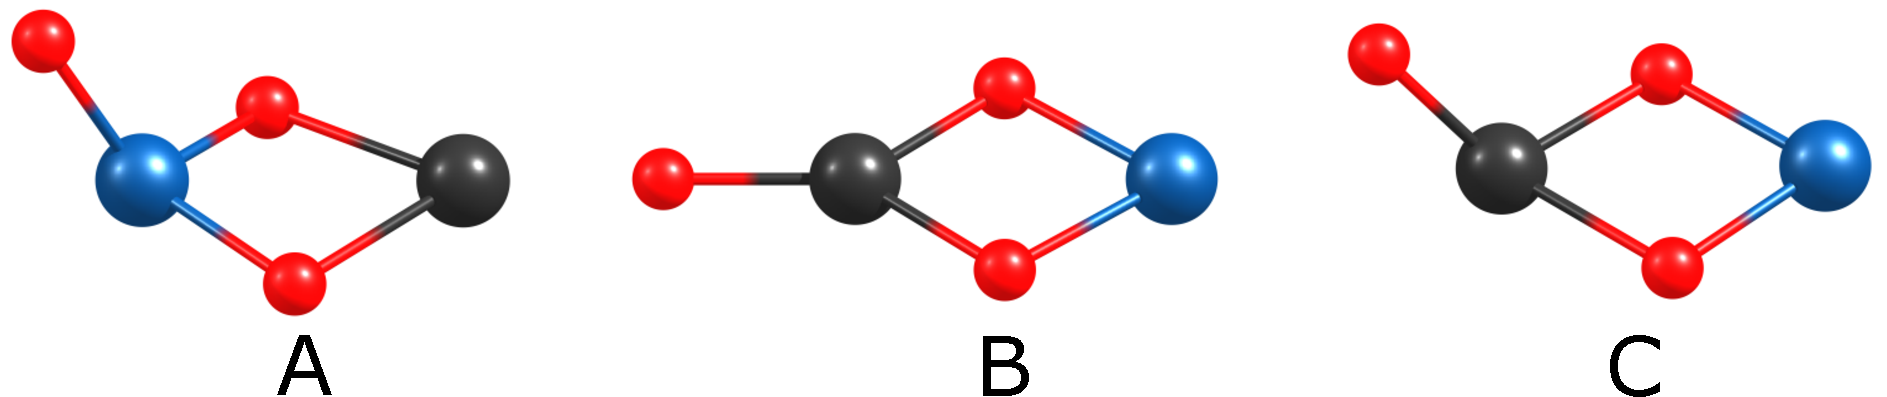
\includegraphics[scale=0.16]{CrMnO3-iso}
		\caption{Geometrical structures of the lowest energy isomers of \ch{CrMnO3+}. The shown structures are obtained with the TPSS/def2TZVP optimizations. Chromium, manganese, and oxygen atoms are represented as blue, black, and red spheres, respectively.}
		\label{figs:CrMnO3}
	\end{figure}




	
\begin{table}[]
	\centering
	\caption{Relative energies (in eV) of the low energy isomers of \ch{CrMnO4+} calculated at different DFT levels}
\begin{tabular}{@{}llllll@{}}
\toprule
\multirow{2}{*}{state} & \multirow{2}{*}{isomer} & \multirow{2}{*}{sym.} & \multicolumn{3}{c}{method} \\ \cmidrule(l){4-6} 
         &     &        & TPSS    & B3P86   & BP86   \\ \midrule
$^5$A    & A   & C$_1$  & 0.00    & 0.00    & 0.00   \\
$^7$A    & A   & C$_1$  & 1.17    & 0.72    & 1.17   \\
$^3$A    & B   & C$_1$  & 0.66    & 0.88    & 0.66   \\
$^5$A    & B   & C$_1$  & 0.68    & 0.86    & 0.68   \\
$^3$A    & C   & C$_1$  & 0.67    & 0.85    & 0.67   \\ \bottomrule
\end{tabular}
\label{tbl:CrMnO4}
\end{table}	



\begin{figure}
	\centering
	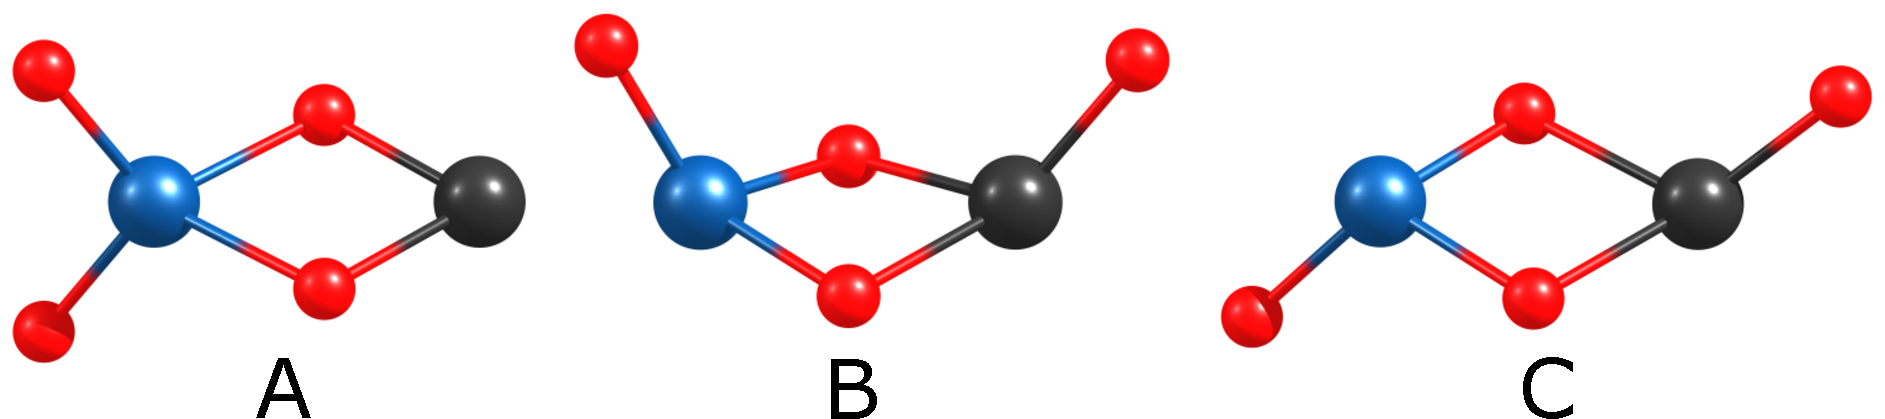
\includegraphics[scale=0.16]{CrMnO4-iso}
	\caption{Geometrical structures of the lowest energy isomers of \ch{CrMnO4+}. The shown structures are obtained with the TPSS/def2TZVP optimizations. Chromium, manganese, and oxygen atoms are represented as blue, black, and red spheres, respectively.}
	\label{figs:CrMnO4}
\end{figure}






\begin{table}[]
	\centering
	\caption{Relative energies (in eV) of the low energy isomers of \ch{CrMn2O5+} calculated at different DFT levels}
\begin{tabular}{@{}llllll@{}}
\toprule
\multirow{2}{*}{state} & \multirow{2}{*}{isomer} & \multirow{2}{*}{sym.} & \multicolumn{3}{c}{method} \\ \cmidrule(l){4-6} 
           &        &         & TPSS   & B3P86 & BP86   \\ \midrule
$^4$A      & A      & C$_1$   & 0.00   & 0.00  & 0.03 \\
$^2$A      & A      & C$_1$   & 0.07   & 0.44  & 0.12 \\
$^8$A      & A      & C$_1$   & 0.12   & 0.05  & 0.18 \\
$^{10}$A   & A      & C$_1$   & 0.22   & 0.09  & 0.34 \\
$^2$A      & B      & C$_1$   & 0.16   & 0.12  & 0.00 \\ \bottomrule
\end{tabular}
\label{tbl:CrMn2O5}
\end{table}	




\begin{figure}
	\centering
	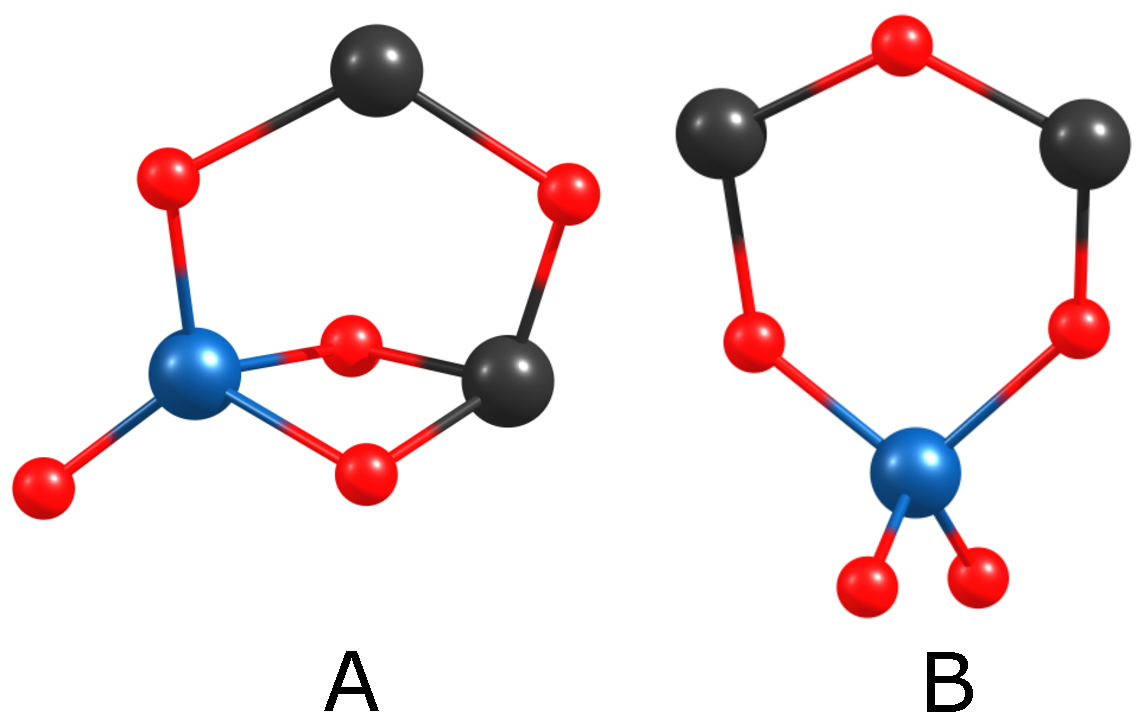
\includegraphics[scale=0.16]{CrMn2O5-iso}
	\caption{Geometrical structures of the lowest energy isomers of \ch{CrMn2O5+}. The shown structures are obtained with the TPSS/def2TZVP optimizations. Chromium, manganese, and oxygen atoms are represented as blue, black, and red spheres, respectively.}
	\label{figs:CrMn2O5}
\end{figure}








\begin{table}[]
	\centering
	\caption{Relative energies (in eV) of the low energy isomers of \ch{CrMn2O6+} calculated at different DFT levels}
\begin{tabular}{@{}llllll@{}}
\toprule
\multirow{2}{*}{state} & \multirow{2}{*}{isomer} & \multirow{2}{*}{sym.} & \multicolumn{3}{c}{method} \\ \cmidrule(l){4-6} 
           &        &         & TPSS   & B3P86 & BP86   \\ \midrule
$^4$A    & A      & C$_1$   & 0.00   & 0.00  & 0.00 \\
$^6$A    & A      & C$_1$   & 0.20   & 0.33  & 0.24 \\
$^8$A    & A      & C$_1$   & 0.19   & 0.12  & 0.23 \\
$^6$A    & B      & C$_1$   & 0.51   & 0.61  & 0.55 \\
$^8$A    & C      & C$_1$   & 0.45   & 0.45  & 0.30 \\ \bottomrule
\end{tabular}
\label{tbl:CrMn2O6}
\end{table}	


\begin{figure}
	\centering
	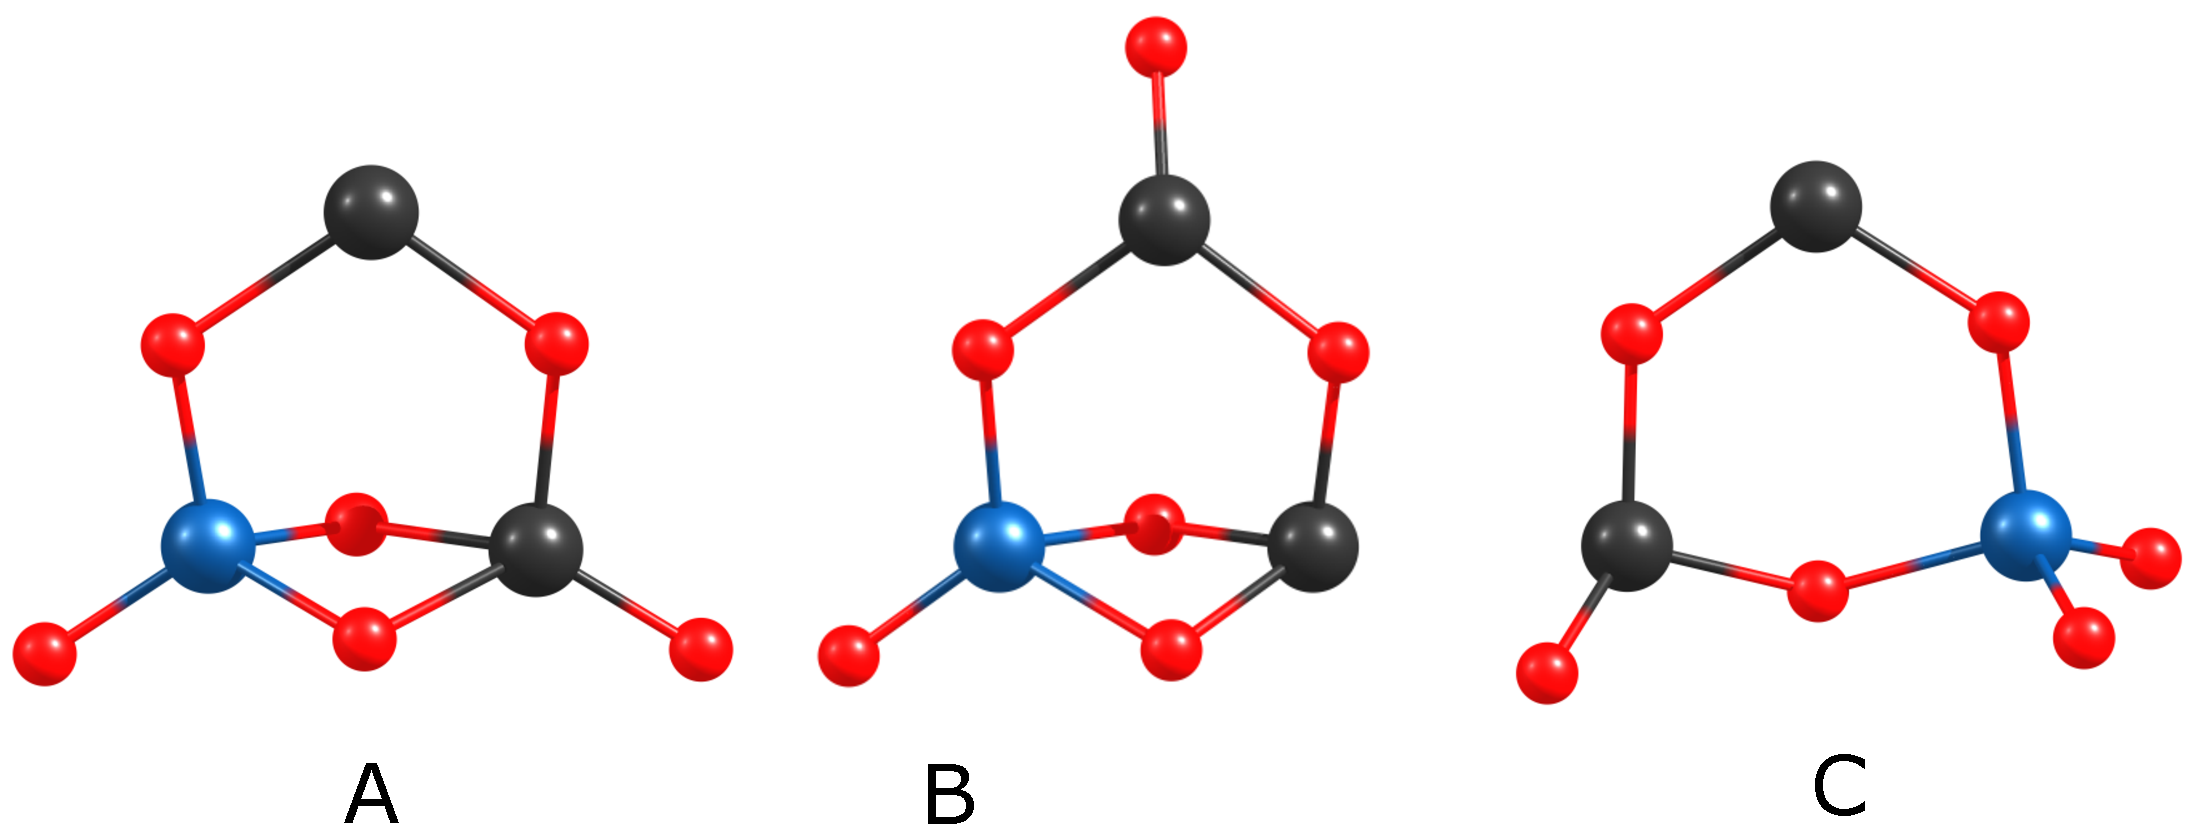
\includegraphics[scale=0.16]{CrMn2O6-iso}
	\caption{Geometrical structures of the lowest energy isomers of \ch{CrMn2O6+}. The shown structures are obtained with the TPSS/def2TZVP optimizations. Chromium, manganese, and oxygen atoms are represented as blue, black, and red spheres, respectively.}
	\label{figs:CrMn2O6}
\end{figure}






\begin{table}[]
	\centering
	\caption{Relative energies (in eV) of the low energy isomers of \ch{Cr2MnO6+} calculated at different DFT levels}
\begin{tabular}{@{}llllll@{}}
\toprule
\multirow{2}{*}{state} & \multirow{2}{*}{isomer} & \multirow{2}{*}{sym.} & \multicolumn{3}{c}{method} \\ \cmidrule(l){4-6} 
         &        &         & TPSS   & B3P86 & BP86   \\ \midrule
$^7$A    & A      & C$_1$   & 0.00   & 0.01  & 0.00 \\
$^5$A    & A      & C$_1$   & 0.00   & 0.00  & 0.03 \\
$^5$A    & B      & C$_1$   & 0.62   & 0.64  & 0.52 \\
$^7$A    & B      & C$_1$   & 0.63   & 0.64  & 0.52 \\
$^7$A    & C      & C$_1$   & 0.70   & 0.67  & 0.72 \\ \bottomrule
\end{tabular}
\label{tbl:Cr2MnO6}
\end{table}	



\begin{figure}
	\centering
	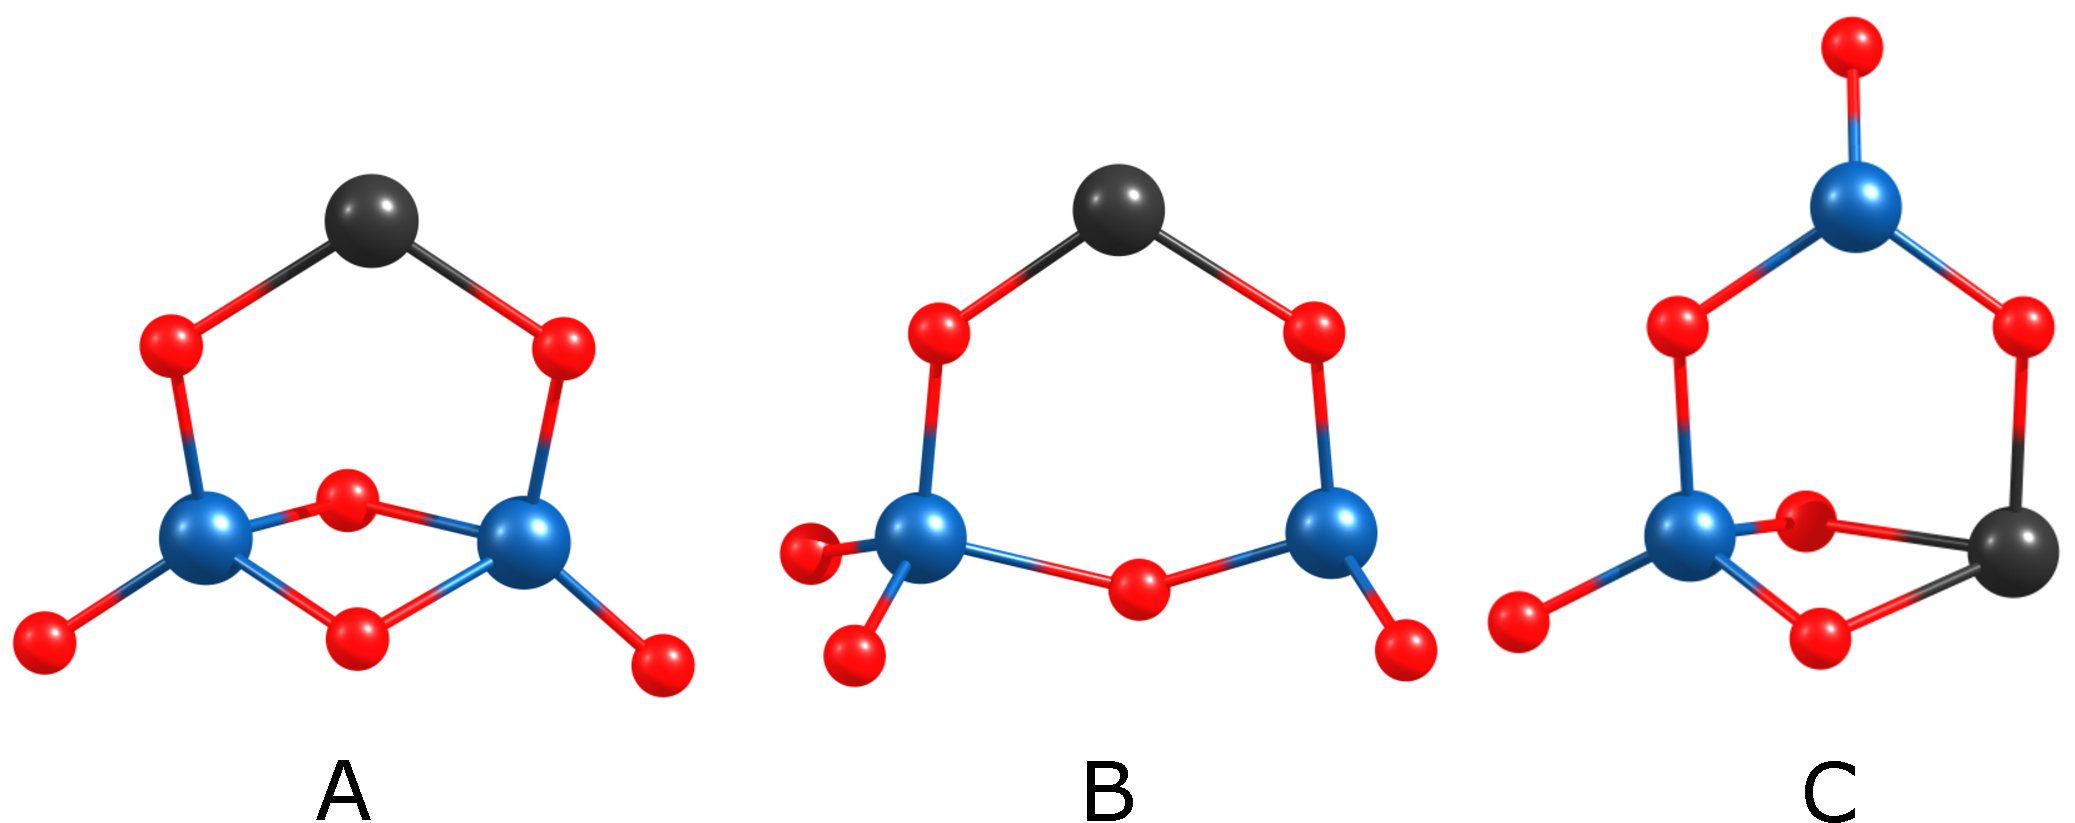
\includegraphics[scale=0.16]{Cr2MnO6-iso}
	\caption{Geometrical structures of the lowest energy isomers of \ch{Cr2MnO6+}. The shown structures are obtained with the TPSS/def2TZVP optimizations. Chromium, manganese, and oxygen atoms are represented as blue, black, and red spheres, respectively.}
	\label{figs:Cr2MnO6}
\end{figure}




\begin{table}[]
	\centering
	\caption{Relative energies (in eV) of the low energy isomers of \ch{Cr2MnO7+} calculated at different DFT levels}
\begin{tabular}{@{}llllll@{}}
\toprule
\multirow{2}{*}{state} & \multirow{2}{*}{isomer} & \multirow{2}{*}{sym.} & \multicolumn{3}{c}{method} \\ \cmidrule(l){4-6} 
         &        &         & TPSS   & B3P86 & BP86   \\ \midrule
$^3$A    & A      & C$_1$   & 0.00   & 0.16  & 0.00 \\
$^5$A    & A      & C$_1$   & 0.09   & 0.28  & 0.09 \\
$^5$A    & B      & C$_1$   & 0.01   & 0.06  & 0.07 \\
$^7$A    & B      & C$_1$   & 0.76   & 0.48  & 0.86 \\
$^5$A    & C      & C$_1$   & 0.15   & 0.00  & 0.14 \\ \bottomrule
\end{tabular}
\label{tbl:Cr2MnO7}
\end{table}	



\begin{figure}
	\centering
	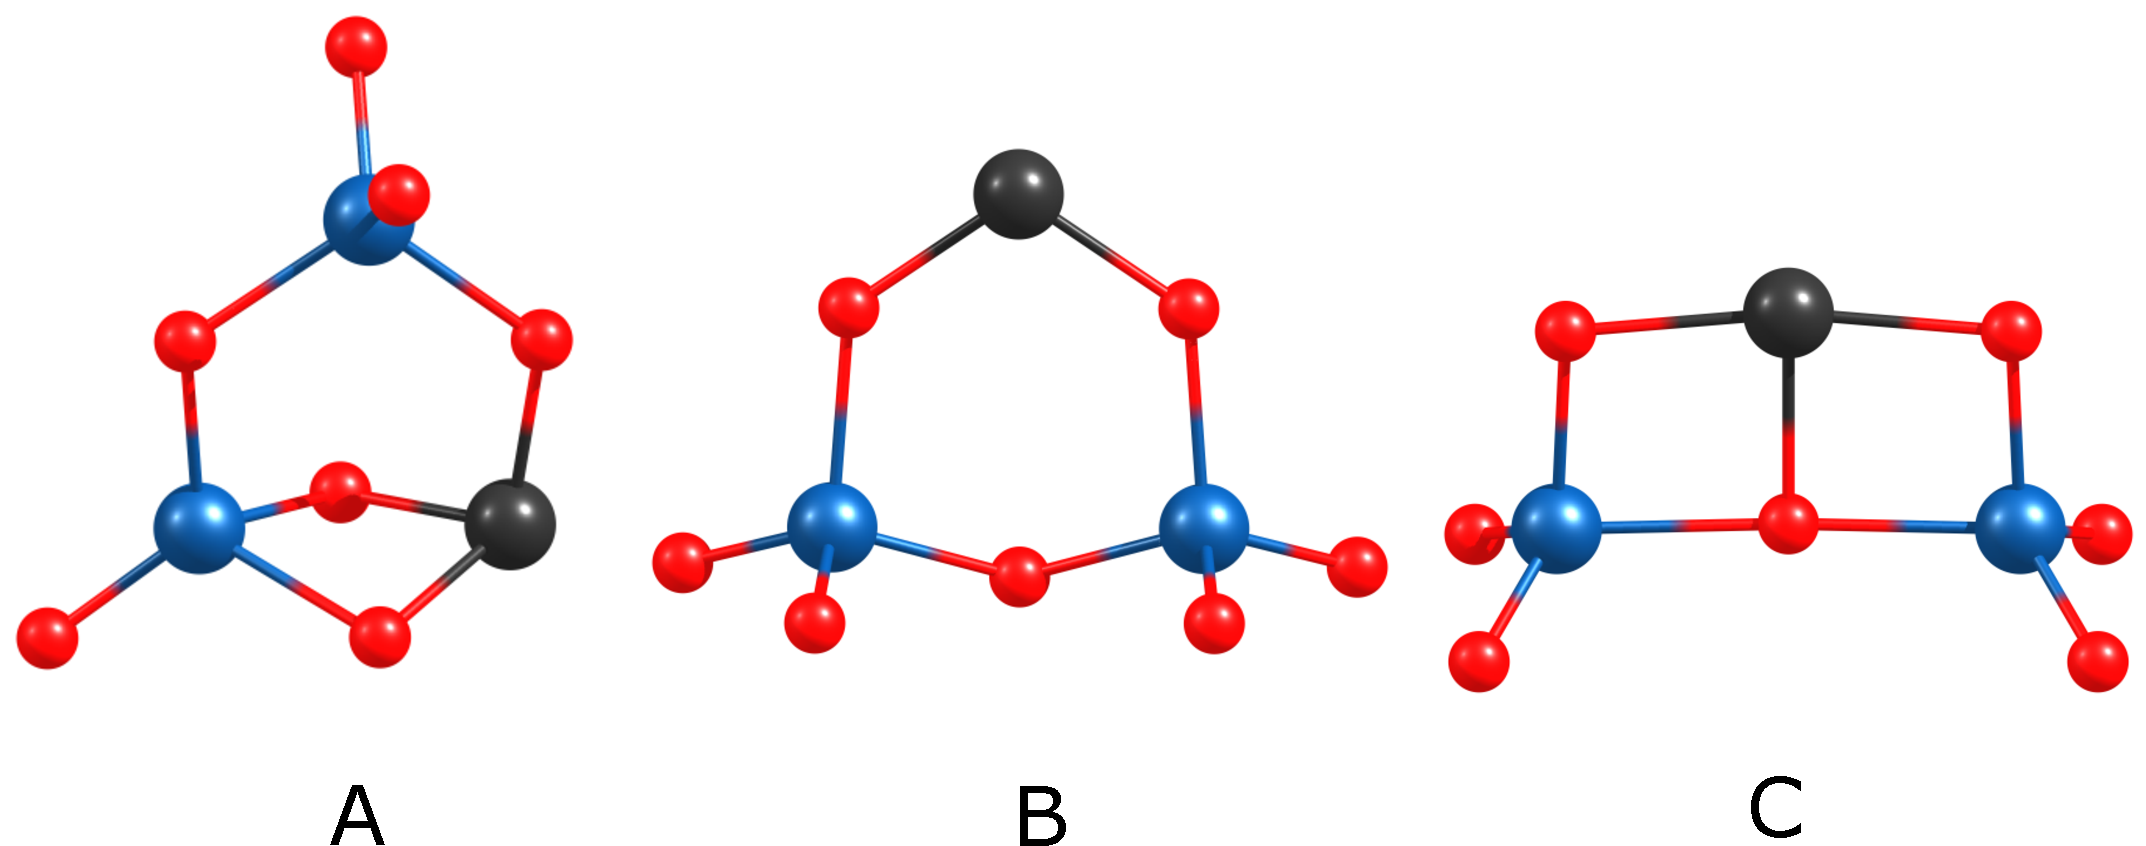
\includegraphics[scale=0.16]{Cr2MnO7-iso}
	\caption{Geometrical structures of the lowest energy isomers of \ch{Cr2MnO7+}. The shown structures are obtained with the TPSS/def2TZVP optimizations. Chromium, manganese, and oxygen atoms are represented as blue, black, and red spheres, respectively.}
	\label{figs:Cr2MnO7}
\end{figure}



\begin{table}[]
	\centering
	\caption{Relative energies (in eV) of the low energy isomers of \ch{CrMn3O6+} calculated at different DFT levels}
\begin{tabular}{@{}llllll@{}}
\toprule
\multirow{2}{*}{state} & \multirow{2}{*}{isomer} & \multirow{2}{*}{sym.} & \multicolumn{3}{c}{method} \\ \cmidrule(l){4-6} 
         &        &         & TPSS   & B3P86 & BP86   \\ \midrule
$^3$A      & A      & C$_1$   & 0.00   & 1.62  & 0.05 \\
$^5$A      & A      & C$_1$   & 0.27   & 0.83  & 0.44 \\
$^7$A      & A      & C$_1$   & 0.07   & 0.91  & 0.24 \\
$^9$A      & A      & C$_1$   & 0.18   & 0.28  & 0.45 \\
$^{13}$A   & A      & C$_1$   & 0.05   & 0.31  & 0.27 \\
$^{13}$A   & B      & C$_1$   & 0.64   & 0.02  & 0.91 \\
$^{15}$A   & B      & C$_1$   & 0.63   & 0.00  & 0.90 \\
$^5$A      & C      & C$_1$   & 1.02   & 0.99  & 0.00 \\ \bottomrule
\end{tabular}
\label{tbl:CrMn3O6}
\end{table}	


\begin{figure}
	\centering
	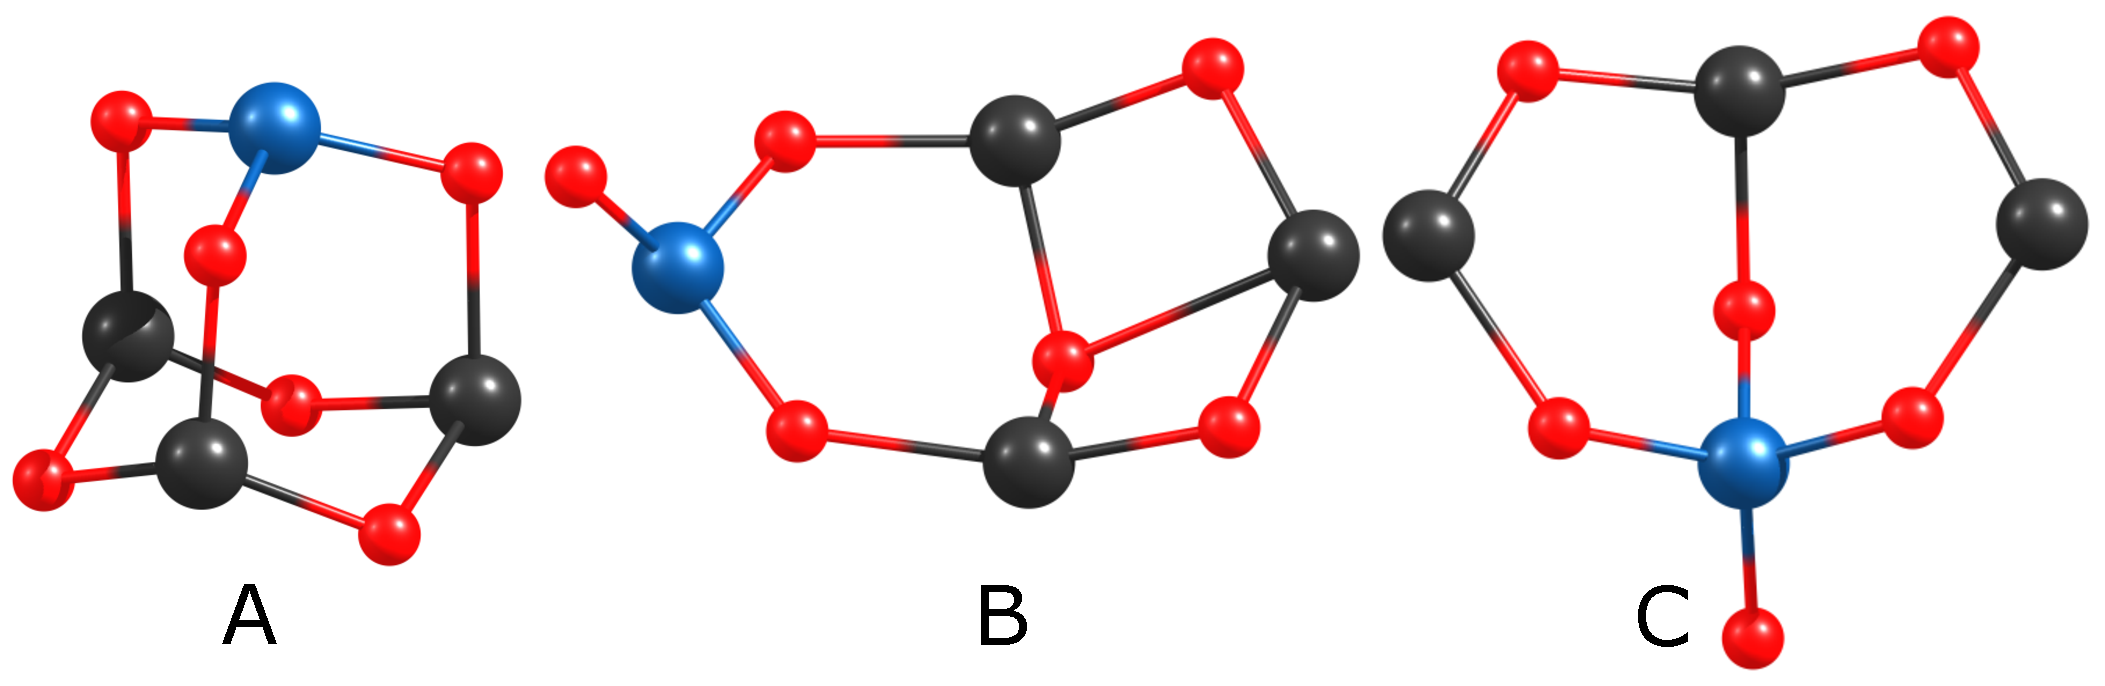
\includegraphics[scale=0.16]{CrMn3O6-iso}
	\caption{Geometrical structures of the lowest energy isomers of \ch{CrMn3O6+}. The shown structures are obtained with the TPSS/def2TZVP optimizations. Chromium, manganese, and oxygen atoms are represented as blue, black, and red spheres, respectively.}
	\label{figs:CrMn3O6}
\end{figure}







\begin{table}[]
	\centering
	\caption{Relative energies (in eV) of the low energy isomers of \ch{CrMn3O7+} calculated at different DFT levels}
\begin{tabular}{@{}llllll@{}}
\toprule
\multirow{2}{*}{state} & \multirow{2}{*}{isomer} & \multirow{2}{*}{sym.} & \multicolumn{3}{c}{method} \\ \cmidrule(l){4-6} 
         &        &         & TPSS   & B3P86 & BP86   \\ \midrule
$^3$A    & A      & C$_1$   & 0.00   & 2.49  & 0.00 \\
$^5$A    & A      & C$_1$   & 0.23   & 1.60  & 0.28 \\
$^5$A    & B      & C$_1$   & 1.49   & 0.00  & 1.68 \\
$^9$A    & B      & C$_1$   & 1.46   & 0.22  & 1.56 \\ \bottomrule
\end{tabular}
\label{tbl:CrMn3O7}
\end{table}	



\begin{figure}
	\centering
	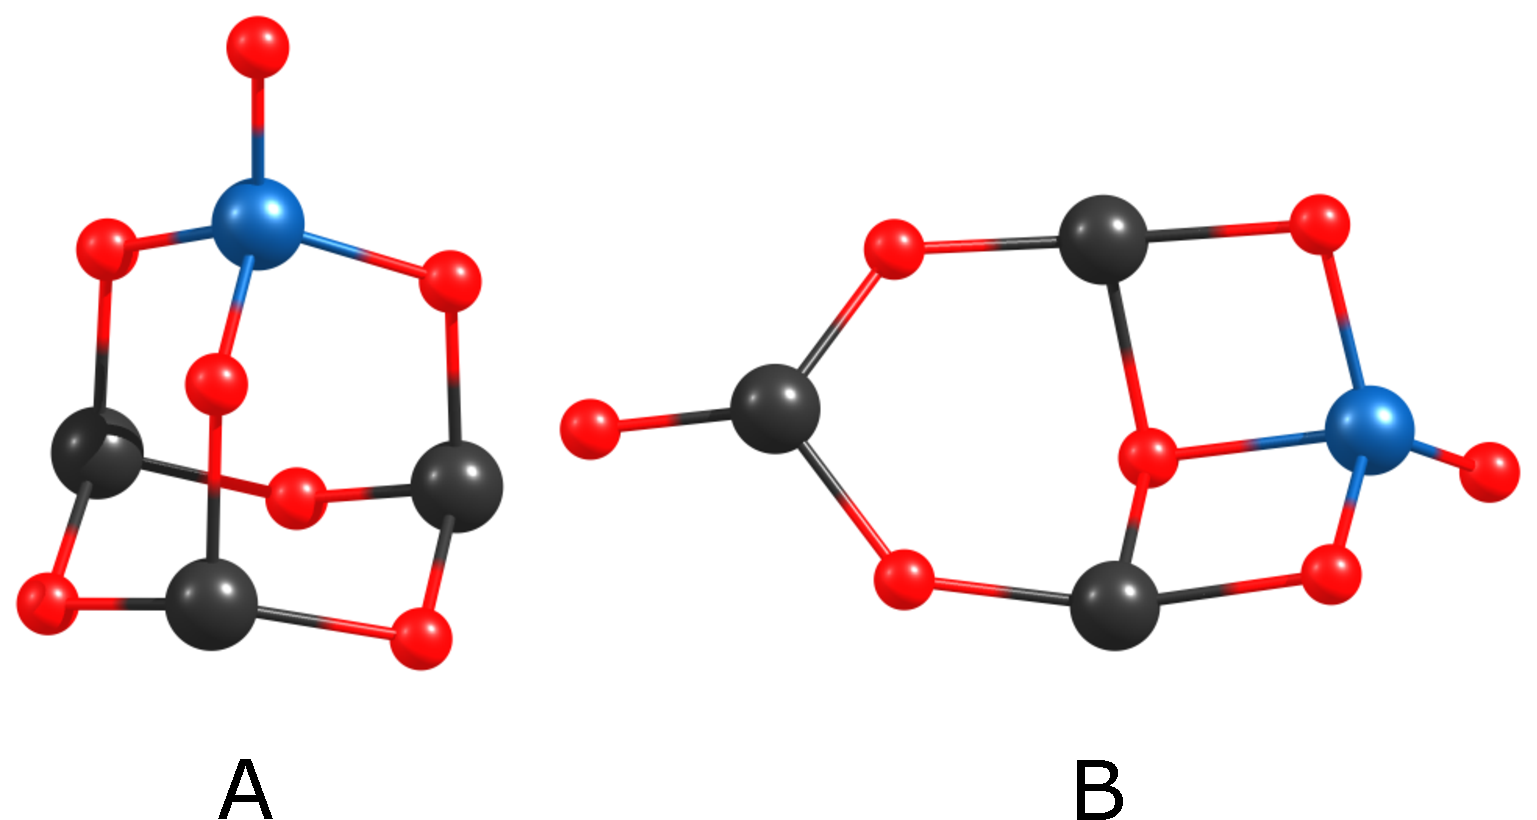
\includegraphics[scale=0.16]{CrMn3O7-iso}
	\caption{Geometrical structures of the lowest energy isomers of \ch{CrMn3O7+}. The shown structures are obtained with the TPSS/def2TZVP optimizations. Chromium, manganese, and oxygen atoms are represented as blue, black, and red spheres, respectively.}
	\label{figs:CrMn3O7}
\end{figure}









\begin{table}[]
	\centering
	\caption{Relative energies (in eV) of the low energy isomers of \ch{Cr2Mn2O7+} calculated at different DFT levels}
\begin{tabular}{@{}llllll@{}}
\toprule
\multirow{2}{*}{state} & \multirow{2}{*}{isomer} & \multirow{2}{*}{sym.} & \multicolumn{3}{c}{method} \\ \cmidrule(l){4-6} 
           &        &         & TPSS   & B3P86 & BP86   \\ \midrule
$^{10}$A   & A      & C$_1$   & 0.00   & 0.00  & 0.01 \\
$^2$A      & B      & C$_1$   & 0.21   & 1.40  & 0.00 \\
$^4$A      & B      & C$_1$   & 0.10   & 0.67  & 0.21 \\
$^6$A      & B      & C$_1$   & 0.35   & 0.68  & 0.54 \\ \bottomrule
\end{tabular}
\label{tbl:Cr2Mn2O7}
\end{table}	


\begin{figure}
	\centering
	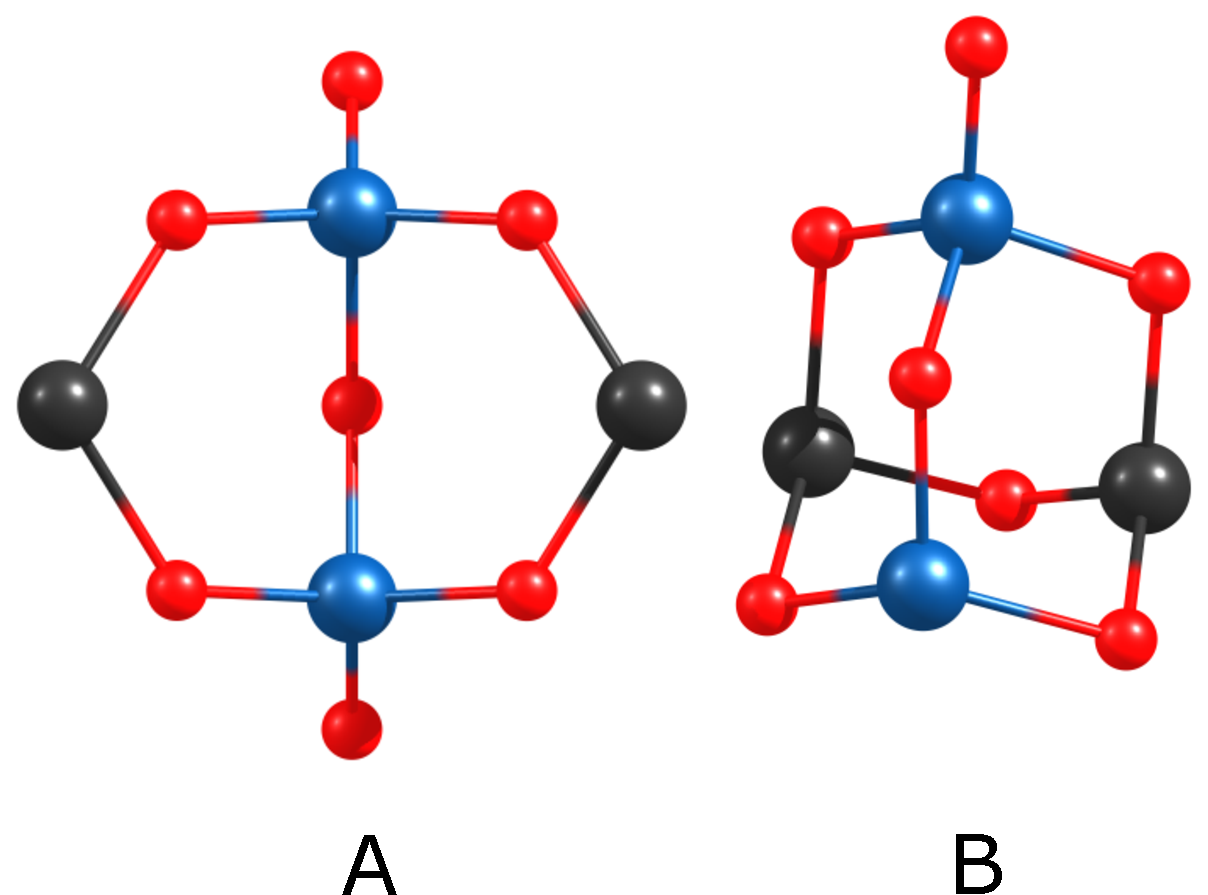
\includegraphics[scale=0.16]{Cr2Mn2O7-iso}
	\caption{Geometrical structures of the lowest energy isomers of \ch{Cr2Mn2O7+}. The shown structures are obtained with the TPSS/def2TZVP optimizations. Chromium, manganese, and oxygen atoms are represented as blue, black, and red spheres, respectively.}
	\label{figs:Cr2Mn2O7}
\end{figure}







\begin{table}[]
	\centering
	\caption{Relative energies (in eV) of the low energy isomers of \ch{Cr2Mn2O8+} calculated at different DFT levels}
\begin{tabular}{@{}llllll@{}}
\toprule
\multirow{2}{*}{state} & \multirow{2}{*}{isomer} & \multirow{2}{*}{sym.} & \multicolumn{3}{c}{method} \\ \cmidrule(l){4-6} 
         &        &         & TPSS   & B3P86 & BP86   \\ \midrule
$^2$A    & A      & C$_1$   & 0.00   & 0.00  & 0.49 \\
$^4$A    & A      & C$_1$   & 0.50   & 1.54  & 0.83 \\
$^6$A    & A      & C$_1$   & 0.47   & 1.02  & 0.00 \\
$^8$A    & A      & C$_1$   & 0.47   & 0.38  & 0.15 \\
$^{10}$A & A      & C$_1$   & 0.54   & 0.14  & 0.26 \\
$^6$A    & B      & C$_1$   & 1.64   & 1.34  & 1.18 \\ \bottomrule
\end{tabular}
\label{tbl:Cr2Mn2O8}
\end{table}	


\begin{figure}
	\centering
	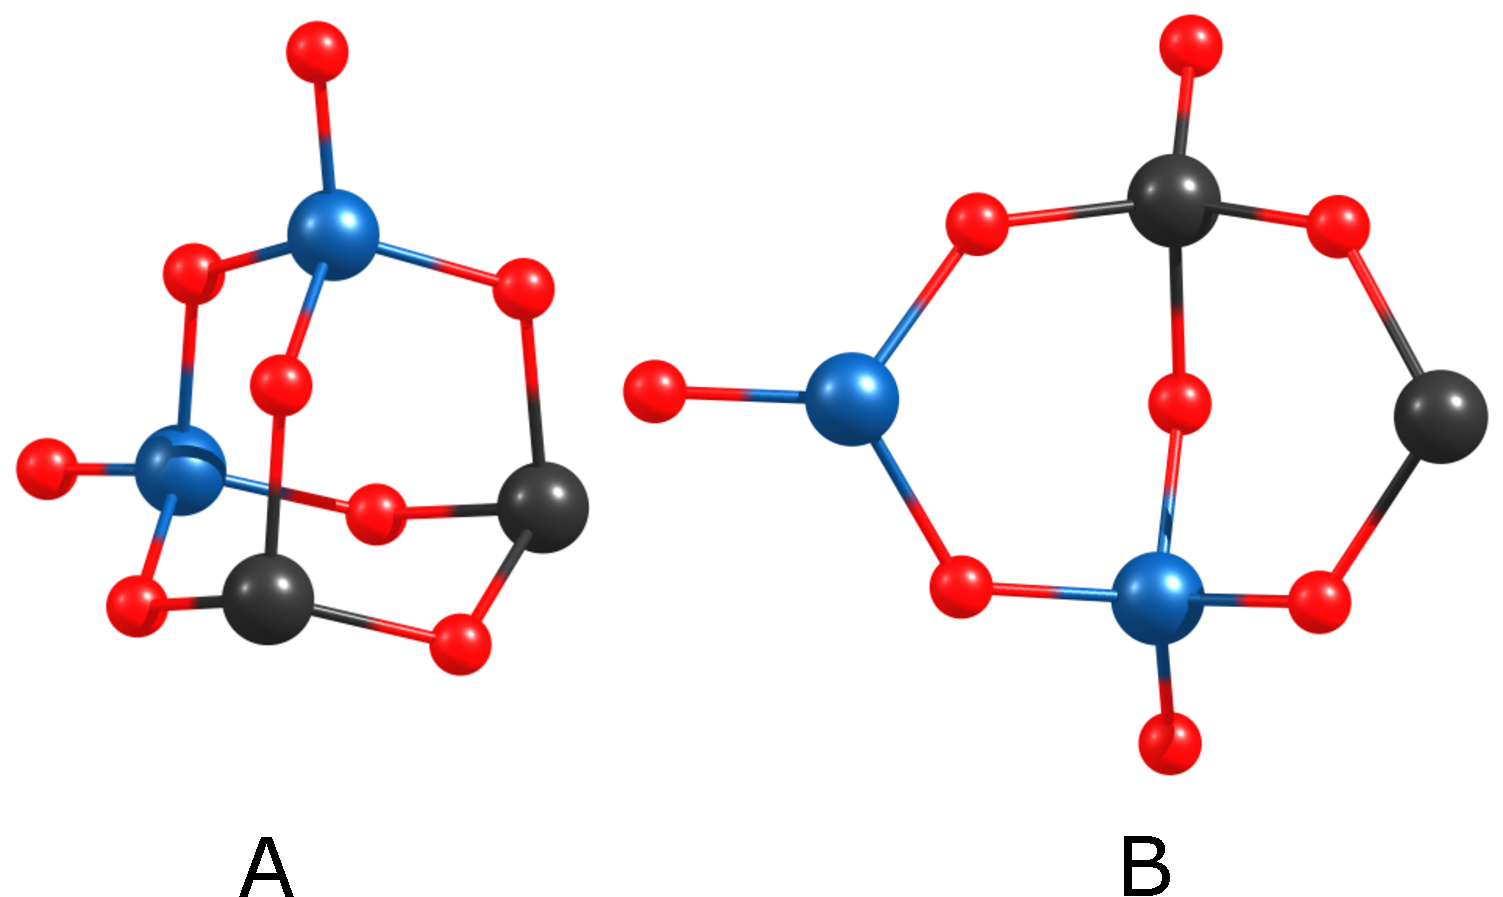
\includegraphics[scale=0.16]{Cr2Mn2O8-iso}
	\caption{Geometrical structures of the lowest energy isomers of \ch{Cr2Mn2O8+}. The shown structures are obtained with the TPSS/def2TZVP optimizations. Chromium, manganese, and oxygen atoms are represented as blue, black, and red spheres, respectively.}
	\label{figs:Cr2Mn2O8}
\end{figure}






\begin{table}[]
	\centering
	\caption{Relative energies (in eV) of the low energy isomers of \ch{Cr3MnO8+} calculated at different DFT levels}
\begin{tabular}{@{}llllll@{}}
\toprule
\multirow{2}{*}{state} & \multirow{2}{*}{isomer} & \multirow{2}{*}{sym.} & \multicolumn{3}{c}{method} \\ \cmidrule(l){4-6} 
         &        &         & TPSS   & B3P86 & BP86   \\ \midrule
$^3$A    & A      & C$_1$   & 0.00   & 0.00  & 0.00 \\
$^5$A    & A      & C$_1$   & 0.36   & 0.76  & 0.21 \\
$^7$A    & A      & C$_1$   & 0.20   & 0.17  & 0.24 \\
$^3$A    & B      & C$_1$   & 0.76   & 0.44  & 0.82 \\
$^5$A    & B      & C$_1$   & 0.92   & 0.47  & 1.08 \\ \bottomrule
\end{tabular}
\label{tbl:Cr3MnO8}
\end{table}	



\begin{figure}
	\centering
	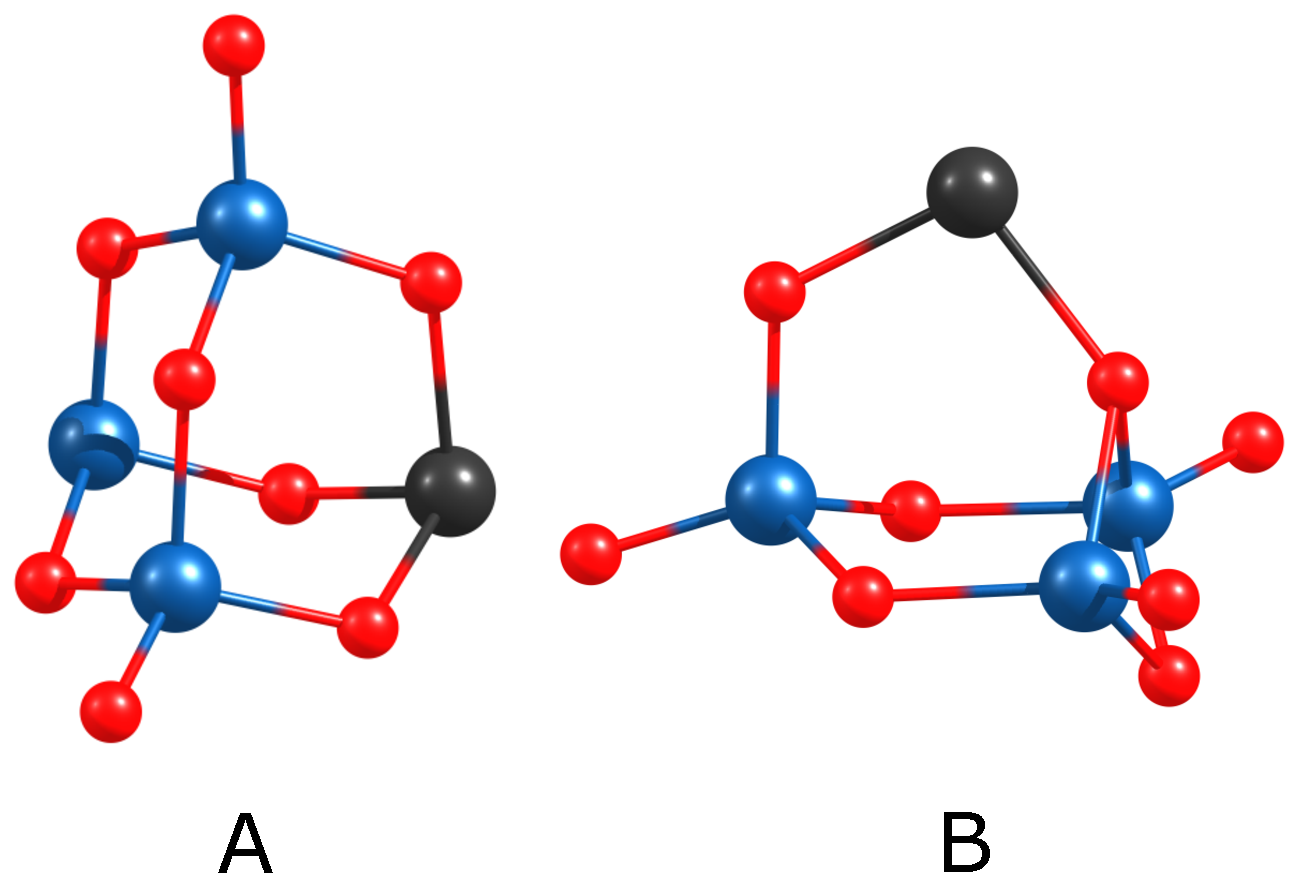
\includegraphics[scale=0.16]{Cr3MnO8-iso}
	\caption{Geometrical structures of the lowest energy isomers of \ch{Cr3MnO8+}. The shown structures are obtained with the TPSS/def2TZVP optimizations. Chromium, manganese, and oxygen atoms are represented as blue, black, and red spheres, respectively.}
	\label{figs:Cr3MnO8}
\end{figure}





\begin{table}[]
	\centering
	\caption{Relative energies (in eV) of the low energy isomers of \ch{Cr3MnO9+} calculated at different DFT levels}
\begin{tabular}{@{}llllll@{}}
\toprule
\multirow{2}{*}{state} & \multirow{2}{*}{isomer} & \multirow{2}{*}{sym.} & \multicolumn{3}{c}{method} \\ \cmidrule(l){4-6} 
         &        &         & TPSS   & B3P86 & BP86   \\ \midrule
$^5$A    & A      & C$_1$   & 0.00   & 0.00  & 0.13 \\
$^7$A    & A      & C$_1$   & 0.36   & 0.12  & 0.00 \\
$^5$A    & B      & C$_1$   & 1.68   & 1.49  & 1.78 \\ \bottomrule
\end{tabular}
\label{tbl:Cr3MnO9}
\end{table}	




\begin{figure}
	\centering
	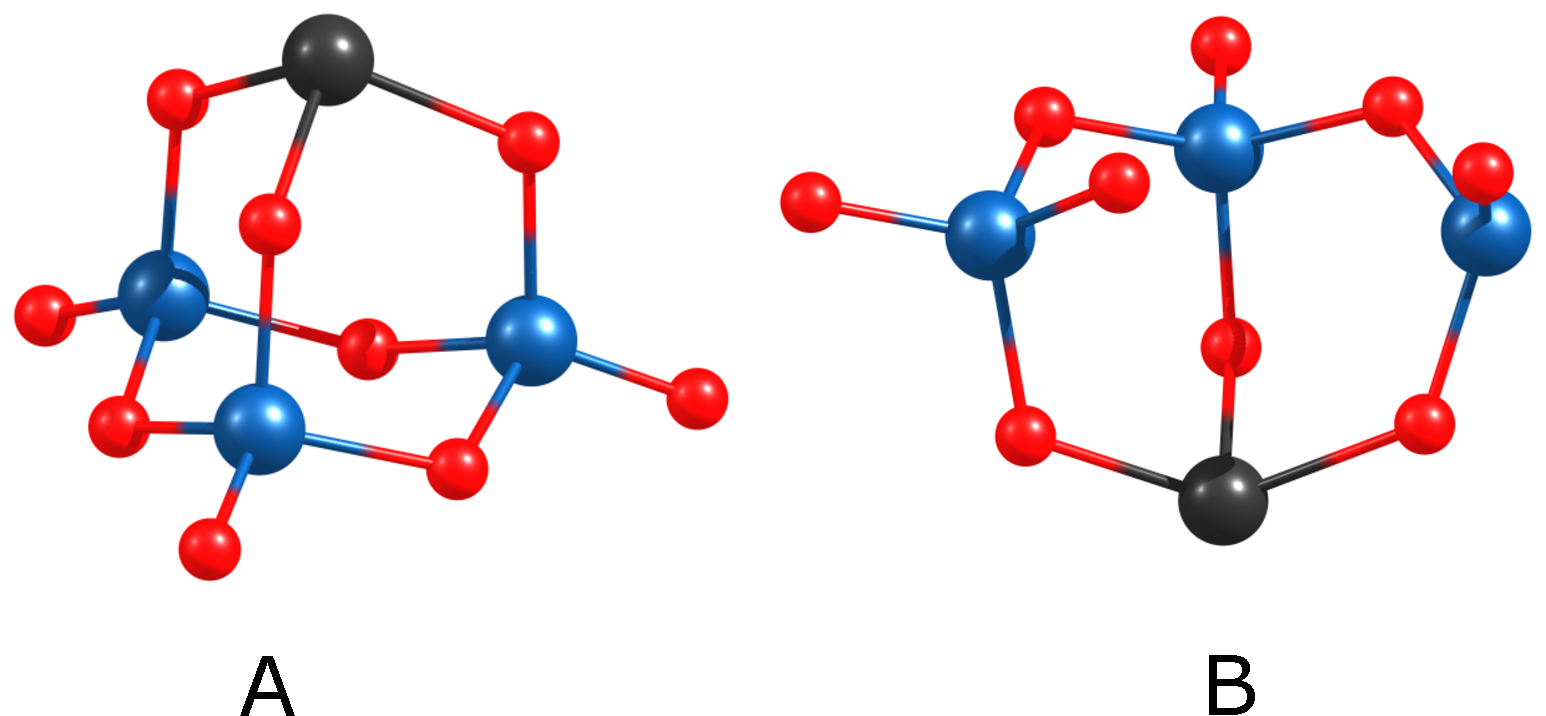
\includegraphics[scale=0.16]{Cr3MnO9-iso}
	\caption{Geometrical structures of the lowest energy isomers of \ch{Cr3MnO9+}. The shown structures are obtained with the TPSS/def2TZVP optimizations. Chromium, manganese, and oxygen atoms are represented as blue, black, and red spheres, respectively.}
	\label{figs:Cr3MnO9}
\end{figure}



\FloatBarrier


\begin{table}[]
	\centering
\caption{Relative energies (in eV) of the low energy isomer of \ch{CrMnO2+} calculated at the TPSS level}
\begin{tabular}{@{}lllc@{}}
\toprule
state 	 & isomer & sym. 	& relative energy (eV) \\ \midrule
$^9$A    & A      & C$_1$   & 0.00                 \\
$^3$A    & A      & C$_1$   & 0.05                 \\
$^5$A    & A      & C$_1$   & 0.49                 \\
$^7$A    & A      & C$_1$   & 0.59                 \\ \bottomrule
\end{tabular}
\end{table}
	




\begin{figure}
	\centering
	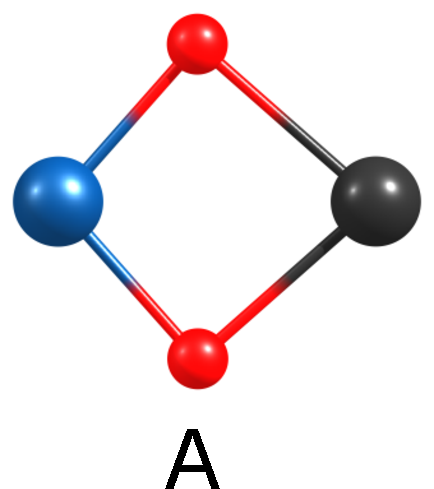
\includegraphics[scale=0.16]{CrMnO2-iso}
	\caption{The geometrical structure of the lowest energy isomer of \ch{CrMnO2+}. The shown structure is obtained with the TPSS/def2TZVP optimizations. Chromium, manganese, and oxygen atoms are represented as blue, black, and red spheres, respectively.}
	\label{figs:CrMnO2}
\end{figure}




\begin{table}[]
	\centering
	\caption{Relative energies (in eV) of the low energy isomers of \ch{CrMnO5+} calculated at the TPSS level}
	\begin{tabular}{@{}lllc@{}}
	\toprule
	state 	 & isomer & sym. 	& relative energy (eV) \\ \midrule
	$^3$A    & A      & C$_1$   & 0.00                 \\
	$^3$A    & B      & C$_1$   & 0.10                 \\
	$^1$A    & C      & C$_1$   & 0.28                 \\
	$^5$A    & C      & C$_1$   & 1.02                 \\ \bottomrule
	\end{tabular}
\end{table}
		


\begin{figure}
	\centering
	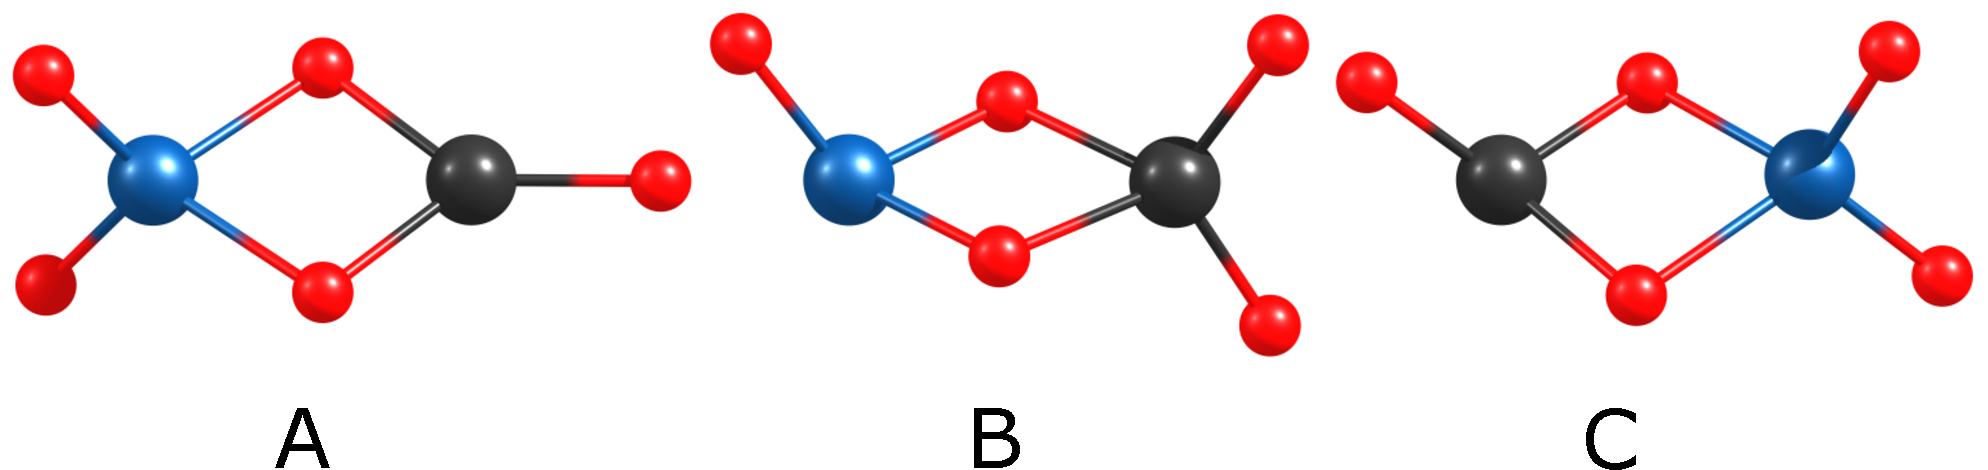
\includegraphics[scale=0.16]{CrMnO5-iso}
	\caption{The geometrical structure of the lowest energy isomer of \ch{CrMnO5+}. The shown structure is obtained with the TPSS/def2TZVP optimizations. Chromium, manganese, and oxygen atoms are represented as blue, black, and red spheres, respectively.}
	\label{figs:CrMnO5}
\end{figure}






\begin{table}[]
	\centering
	\caption{Relative energies (in eV) of the low energy isomer of \ch{CrMnO6+} calculated at the TPSS level}
	\begin{tabular}{@{}lllc@{}}
	\toprule
	state 	 & isomer & sym. 	& relative energy (eV) \\ \midrule
	$^1$A    & A      & C$_1$   & 0.00                 \\
	$^3$A    & A      & C$_1$   & 0.56                 \\ \bottomrule
	\end{tabular}
\end{table}
		




\begin{figure}
	\centering
	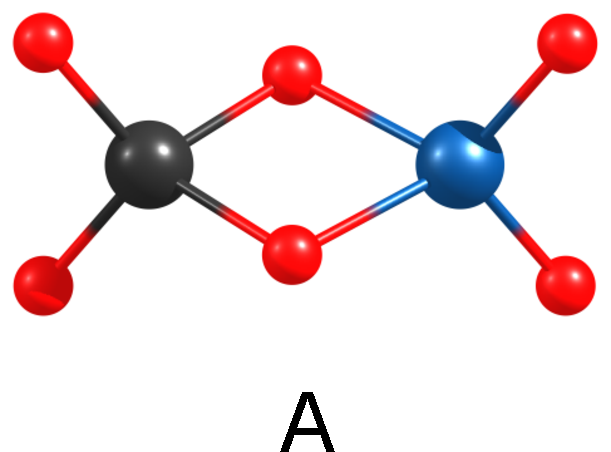
\includegraphics[scale=0.16]{CrMnO6-iso}
	\caption{The geometrical structure of the lowest energy isomer of \ch{CrMnO6+}. The shown structure is obtained with the TPSS/def2TZVP optimizations. Chromium, manganese, and oxygen atoms are represented as blue, black, and red spheres, respectively.}
	\label{figs:CrMnO6}
\end{figure}






\begin{table}[]
	\centering
	\caption{Relative energies (in eV) of the low energy isomers of \ch{CrMn2O4+} calculated at the TPSS level}
	\begin{tabular}{@{}lllc@{}}
	\toprule
	state 	 & isomer & sym. 	& relative energy (eV) \\ \midrule
	$^6$A    & A      & C$_1$   & 0.00                 \\
	$^2$A    & A      & C$_1$   & 0.13                 \\
	$^8$A    & A      & C$_1$   & 0.39                 \\
	$^4$A    & B      & C$_1$   & 0.85                 \\ \bottomrule
	\end{tabular}
\end{table}



\begin{figure}
	\centering
	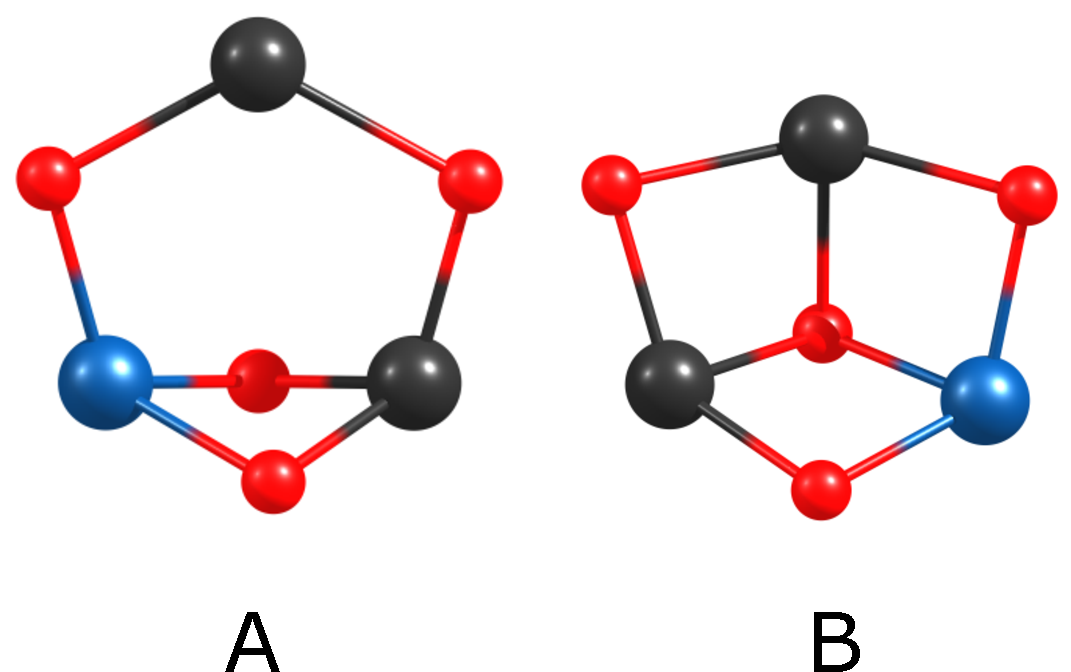
\includegraphics[scale=0.16]{CrMn2O4-iso}
	\caption{The geometrical structure of the lowest energy isomer of \ch{CrMn2O4+}. The shown structures are obtained with the TPSS/def2TZVP optimizations. Chromium, manganese, and oxygen atoms are represented as blue, black, and red spheres, respectively.}
	\label{figs:CrMn2O4}
\end{figure}





\begin{table}[]
	\centering
	\caption{Relative energies (in eV) of the low energy isomers of \ch{CrMn2O7+} calculated at the TPSS level}
	\begin{tabular}{@{}lllc@{}}
	\toprule
	state & isomer & sym. & relative energy (eV) \\ \midrule
	$^6$A    & A      & C$_1$   & 0.00                 \\
	$^4$A    & A      & C$_1$   & 0.05                 \\
	$^2$A    & B      & C$_1$   & 0.30                 \\
	$^4$A    & B      & C$_1$   & 0.38                 \\
	$^6$A    & B      & C$_1$   & 0.41                 \\
	$^2$A    & C      & C$_1$   & 0.47                 \\
	$^4$A    & C      & C$_1$   & 0.48                 \\
	$^6$A    & C      & C$_1$   & 0.48                 \\ \bottomrule
	\end{tabular}
\end{table}


\begin{figure}
	\centering
	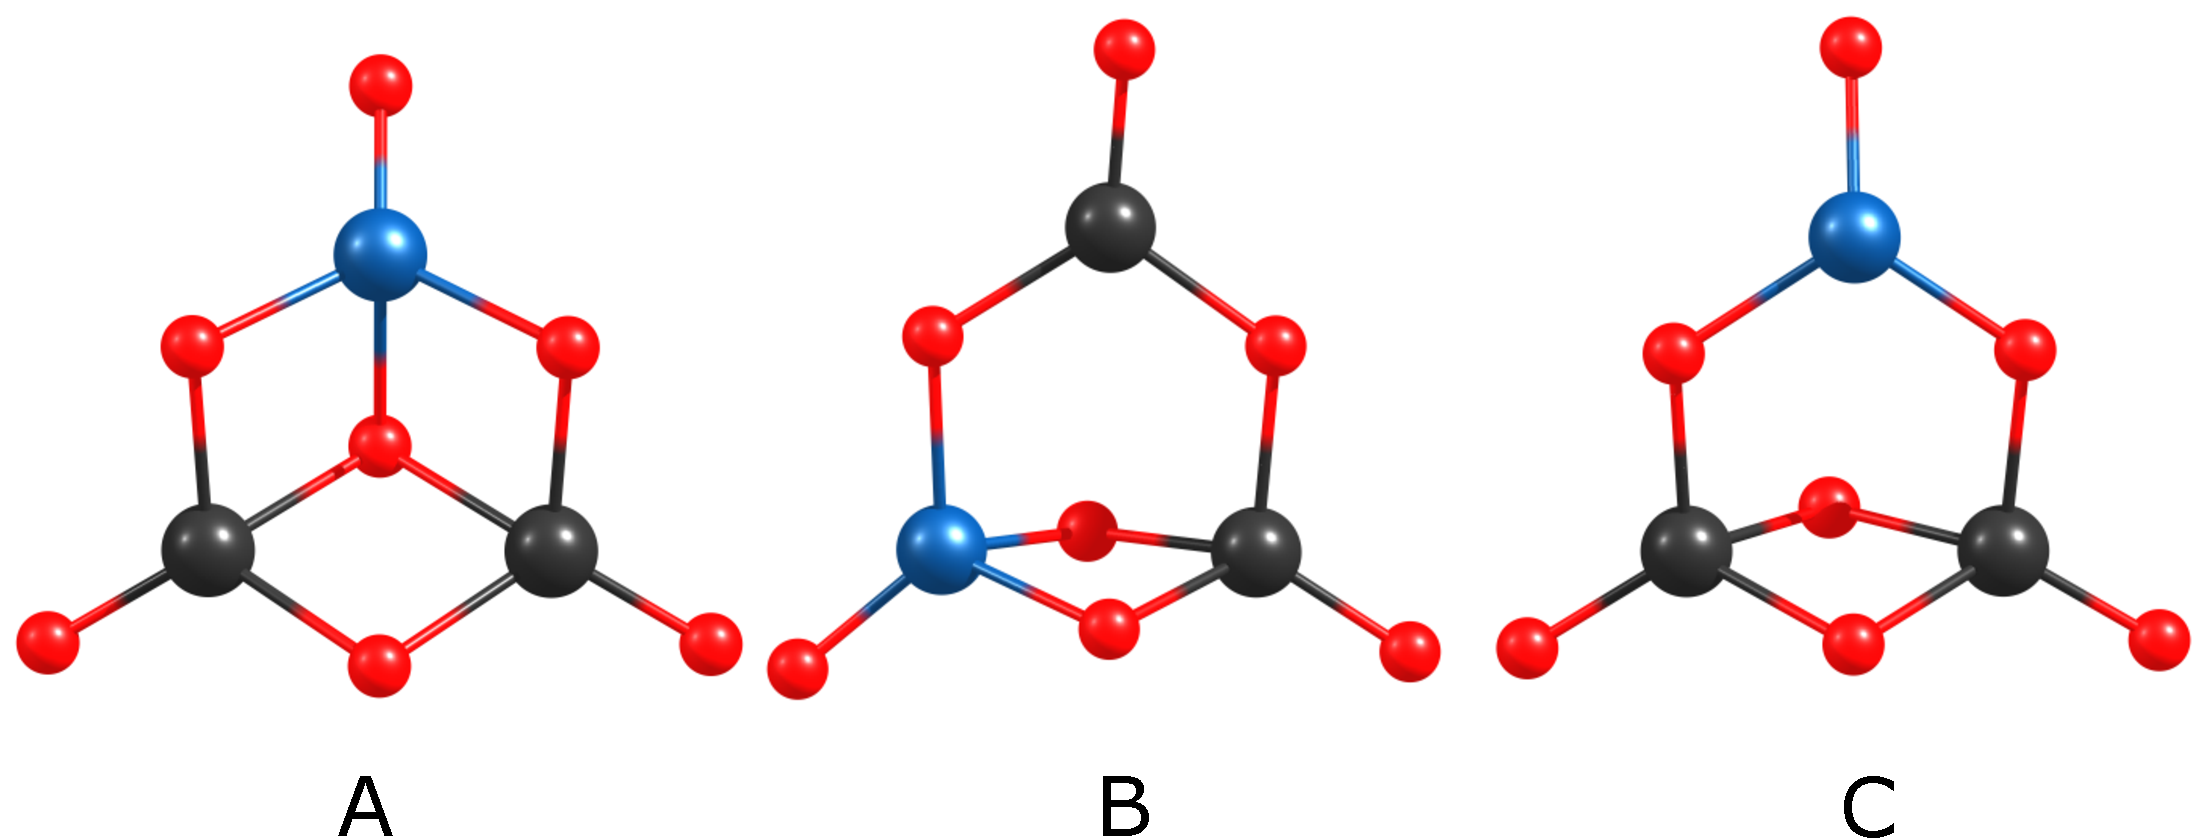
\includegraphics[scale=0.16]{CrMn2O7-iso}
	\caption{The geometrical structure of the lowest energy isomer of \ch{CrMn2O7+}. The shown structures are obtained with the TPSS/def2TZVP optimizations. Chromium, manganese, and oxygen atoms are represented as blue, black, and red spheres, respectively.}
	\label{figs:CrMn2O7}
\end{figure}







\begin{table}[]
	\centering
	\caption{Relative energies (in eV) of the low energy isomers of \ch{CrMn2O8+} calculated at the TPSS level}
	\begin{tabular}{@{}lllc@{}}
	\toprule
	state & isomer & sym. & relative energy (eV) \\ \midrule
	$^2A$    & A      & C$_1$   & 0.00                 \\
	$^4A$    & A      & C$_1$   & 0.08                 \\
	$^4A$    & B      & C$_1$   & 0.53                 \\
	$^2A$    & B      & C$_1$   & 0.68                 \\
	$^4A$    & C      & C$_1$   & 0.81                 \\
	$^2A$    & C      & C$_1$   & 0.83                 \\ \bottomrule
	\end{tabular}
\end{table}


\begin{figure}
	\centering
	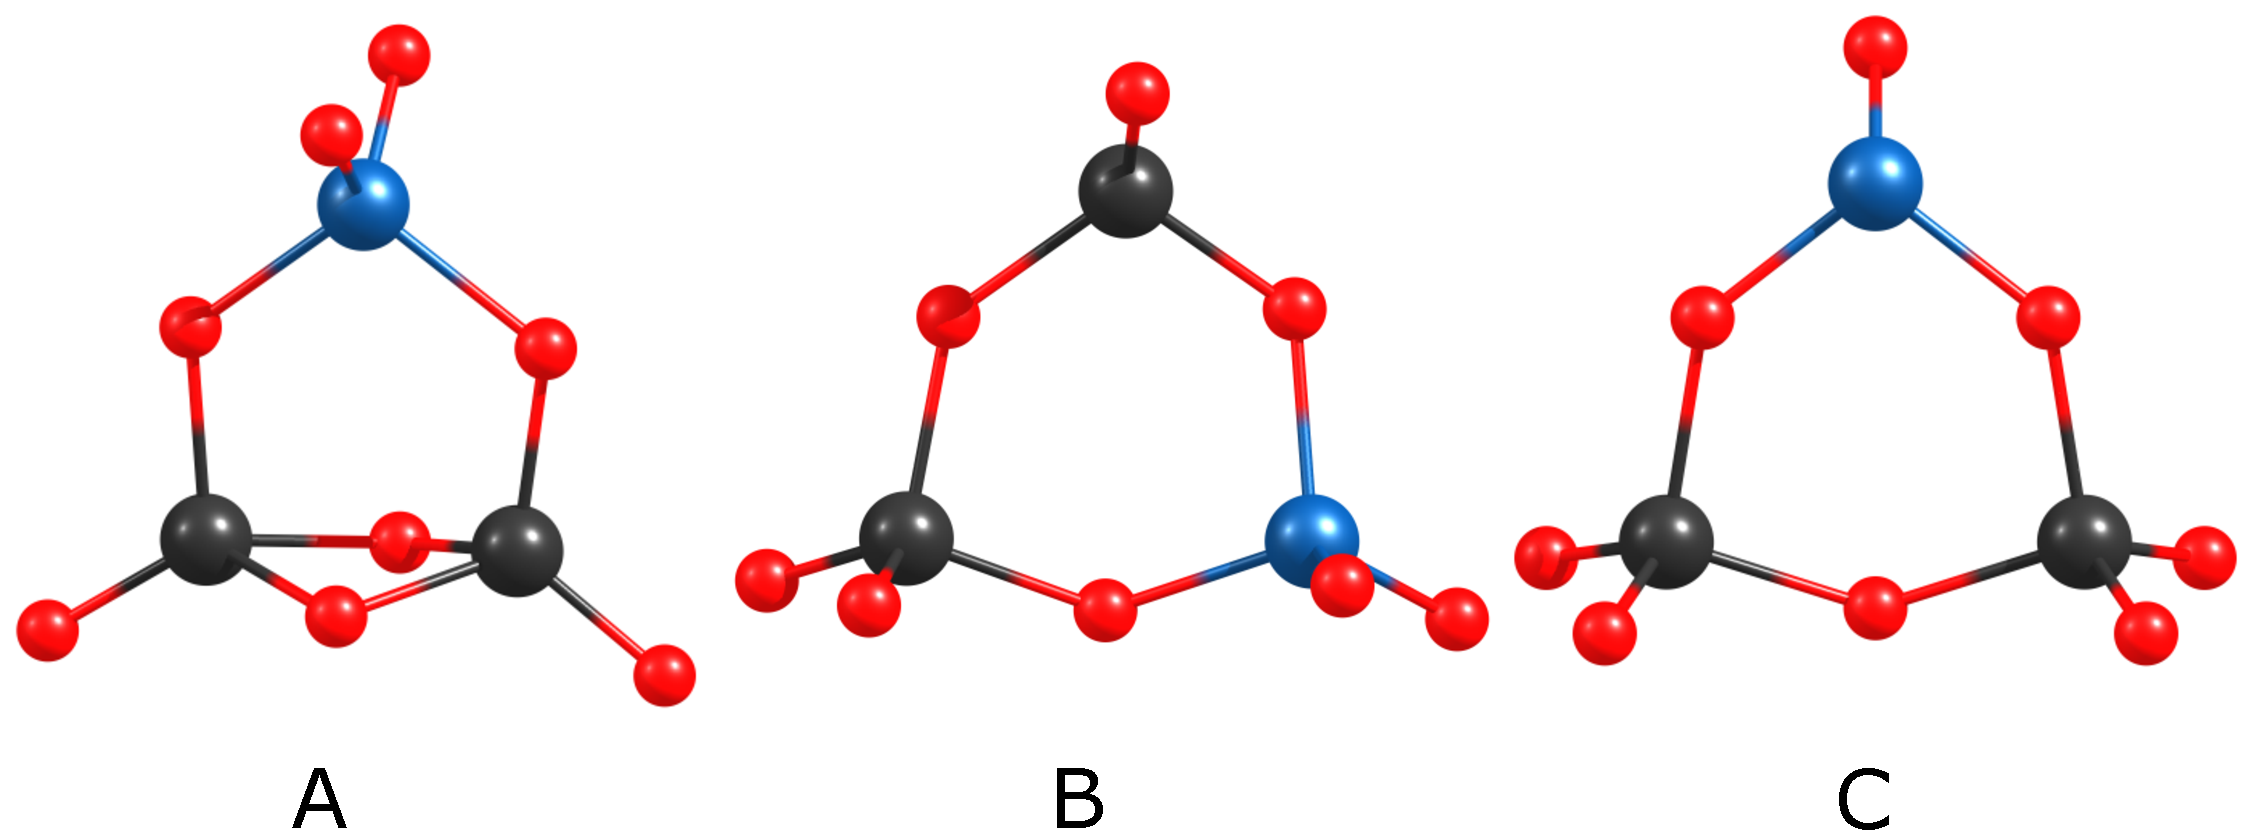
\includegraphics[scale=0.16]{CrMn2O8-iso}
	\caption{The geometrical structure of the lowest energy isomer of \ch{CrMn2O8+}. The shown structures are obtained with the TPSS/def2TZVP optimizations. Chromium, manganese, and oxygen atoms are represented as blue, black, and red spheres, respectively.}
	\label{figs:CrMn2O8}
\end{figure}








\begin{table}[]
	\centering
	\caption{Relative energies (in eV) of the low energy isomers of \ch{Cr2MnO3+} calculated at the TPSS level}
	\begin{tabular}{@{}lllc@{}}
	\toprule
	state & isomer & sym. & relative energy (eV) \\ \midrule
	$^3$A      & A      & C$_1$   & 0.00                 \\
	$^{11}$A   & B      & C$_1$   & 0.49                 \\
	$^7$A      & A      & C$_1$   & 0.51                 \\
	$^1$A      & A      & C$_1$   & 0.74                 \\
	$^9$A      & B      & C$_1$   & 0.82                 \\ \bottomrule
	\end{tabular}
\end{table}



\begin{figure}
	\centering
	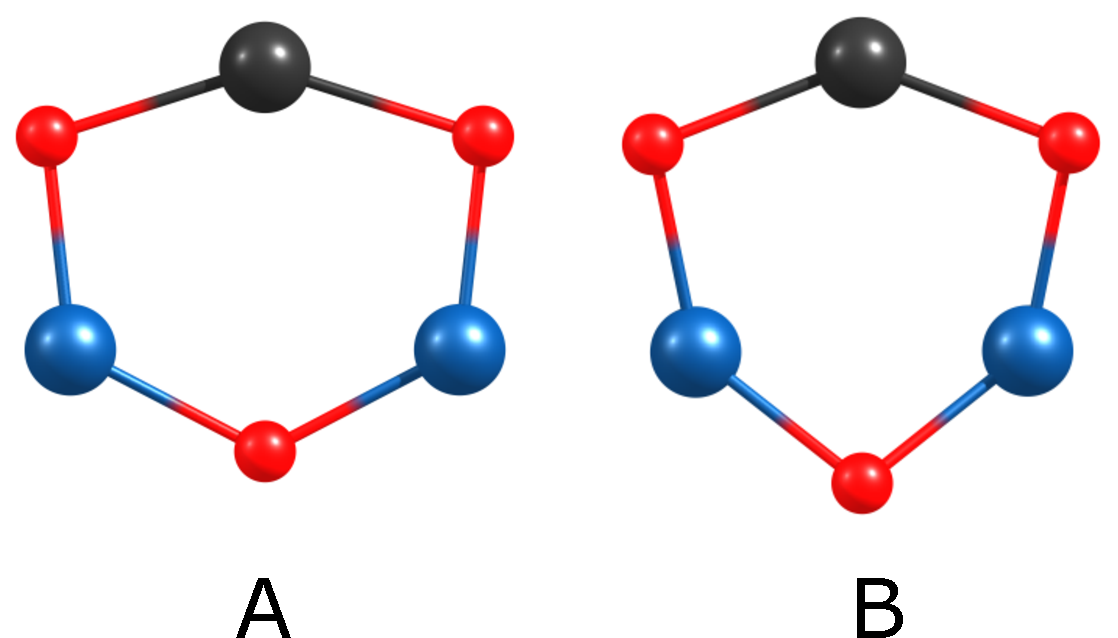
\includegraphics[scale=0.16]{Cr2MnO3-iso}
	\caption{The geometrical structure of the lowest energy isomer of \ch{Cr2MnO3+}. The shown structures are obtained with the TPSS/def2TZVP optimizations. Chromium, manganese, and oxygen atoms are represented as blue, black, and red spheres, respectively.}
	\label{figs:CrMn2O8}
\end{figure}







\begin{table}[]
	\centering
	\caption{Relative energies (in eV) of the low energy isomers of \ch{Cr2MnO4+} calculated at the TPSS level}
	\begin{tabular}{@{}lllc@{}}
	\toprule
	state & isomer & sym. & relative energy (eV) \\ \midrule
	$^3$A    & A      & C$_1$    & 0.00                 \\
	$^5$A    & A      & C$_1$    & 0.01                 \\
	$^9$A    & A      & C$_1$    & 0.18                 \\
	$^7$A    & A      & C$_1$    & 0.20                 \\
	$^3$A    & B      & C$_1$    & 0.33                 \\
	$^1$A    & A      & C$_1$    & 0.38                 \\
	$^5$A    & C      & C$_1$    & 0.68                 \\
	$^3$A    & C      & C$_1$    & 0.73                 \\ \bottomrule
	\end{tabular}
\end{table}

	

\begin{figure}
	\centering
	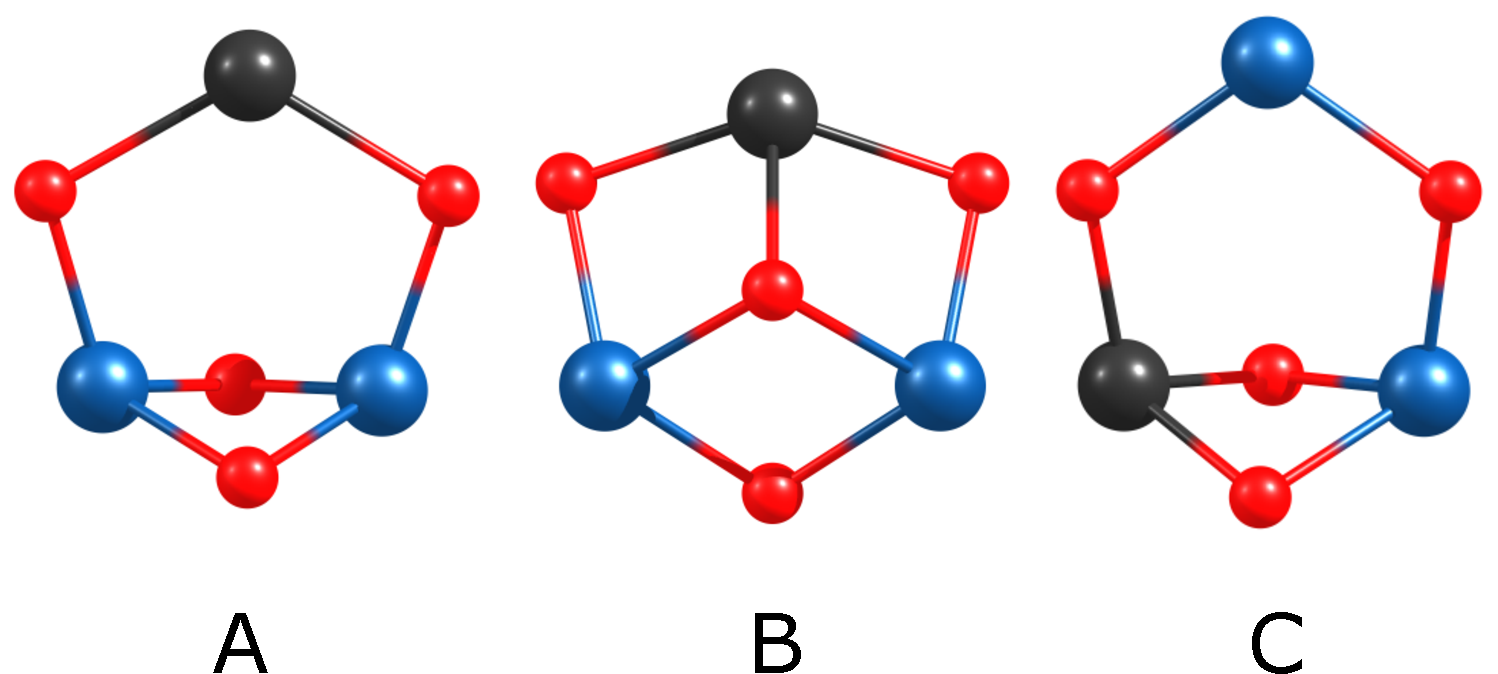
\includegraphics[scale=0.16]{Cr2MnO4-iso}
	\caption{Geometrical structures of the lowest energy isomers of \ch{Cr2MnO4+}. The shown structures are obtained with the TPSS/def2TZVP optimizations. Chromium, manganese, and oxygen atoms are represented as blue, black, and red spheres, respectively.}
	\label{figs:Cr2MnO4}
\end{figure}







\begin{table}[]
	\centering
	\caption{Relative energies (in eV) of the low energy isomers of \ch{Cr2MnO5+} calculated at the TPSS level}
	\begin{tabular}{@{}lllc@{}}
	\toprule
	state & isomer & sym. & relative energy (eV) \\ \midrule
	$^3$A    & A      & C$_1$   & 0.00                 \\
	$^7$A    & A      & C$_1$   & 0.05                 \\
	$^5$A    & A      & C$_1$   & 0.50                 \\
	$^5$A    & B      & C$_1$   & 0.52                 \\
	$^9$A    & B      & C$_1$   & 0.57                 \\
	$^7$A    & B      & C$_1$   & 0.79                 \\
	$^3$A    & C      & C$_1$   & 0.81                 \\ \bottomrule
	\end{tabular}
\end{table}

\begin{figure}
	\centering
	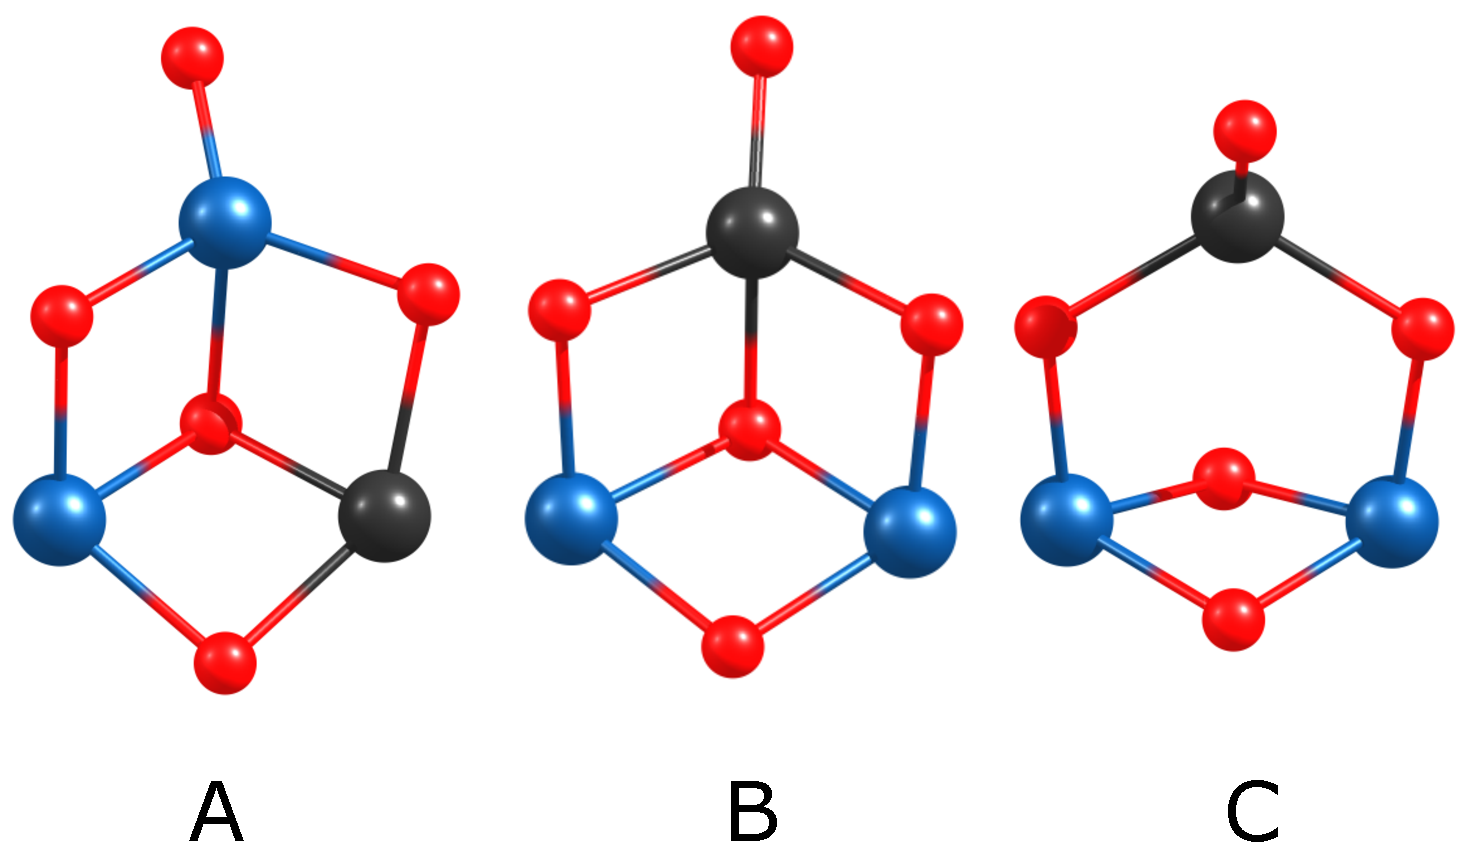
\includegraphics[scale=0.16]{Cr2MnO5-iso}
	\caption{Geometrical structures of the lowest energy isomers of \ch{Cr2MnO5+}. The shown structures are obtained with the TPSS/def2TZVP optimizations. Chromium, manganese, and oxygen atoms are represented as blue, black, and red spheres, respectively.}
	\label{figs:Cr2MnO5}
\end{figure}






\begin{table}[]
	\centering
	\caption{Relative energies (in eV) of the low energy isomers of \ch{Cr2MnO8+} calculated at the TPSS level}
	\begin{tabular}{@{}lllc@{}}
	\toprule
	state & isomer & sym. & relative energy (eV) \\ \midrule
	$^3$A    & A      & C1   & 0.00                 \\
	$^1$A    & A      & C1   & 0.20                 \\
	$^3$A    & B      & C1   & 0.28                 \\
	$^3$A    & C      & C1   & 0.35                 \\
	$^1$A    & C      & C1   & 0.38                 \\
	$^3$A    & D      & C1   & 0.57                 \\
	$^1$A    & B      & C1   & 0.63                 \\ \bottomrule
	\end{tabular}
\end{table}



\begin{figure}
	\centering
	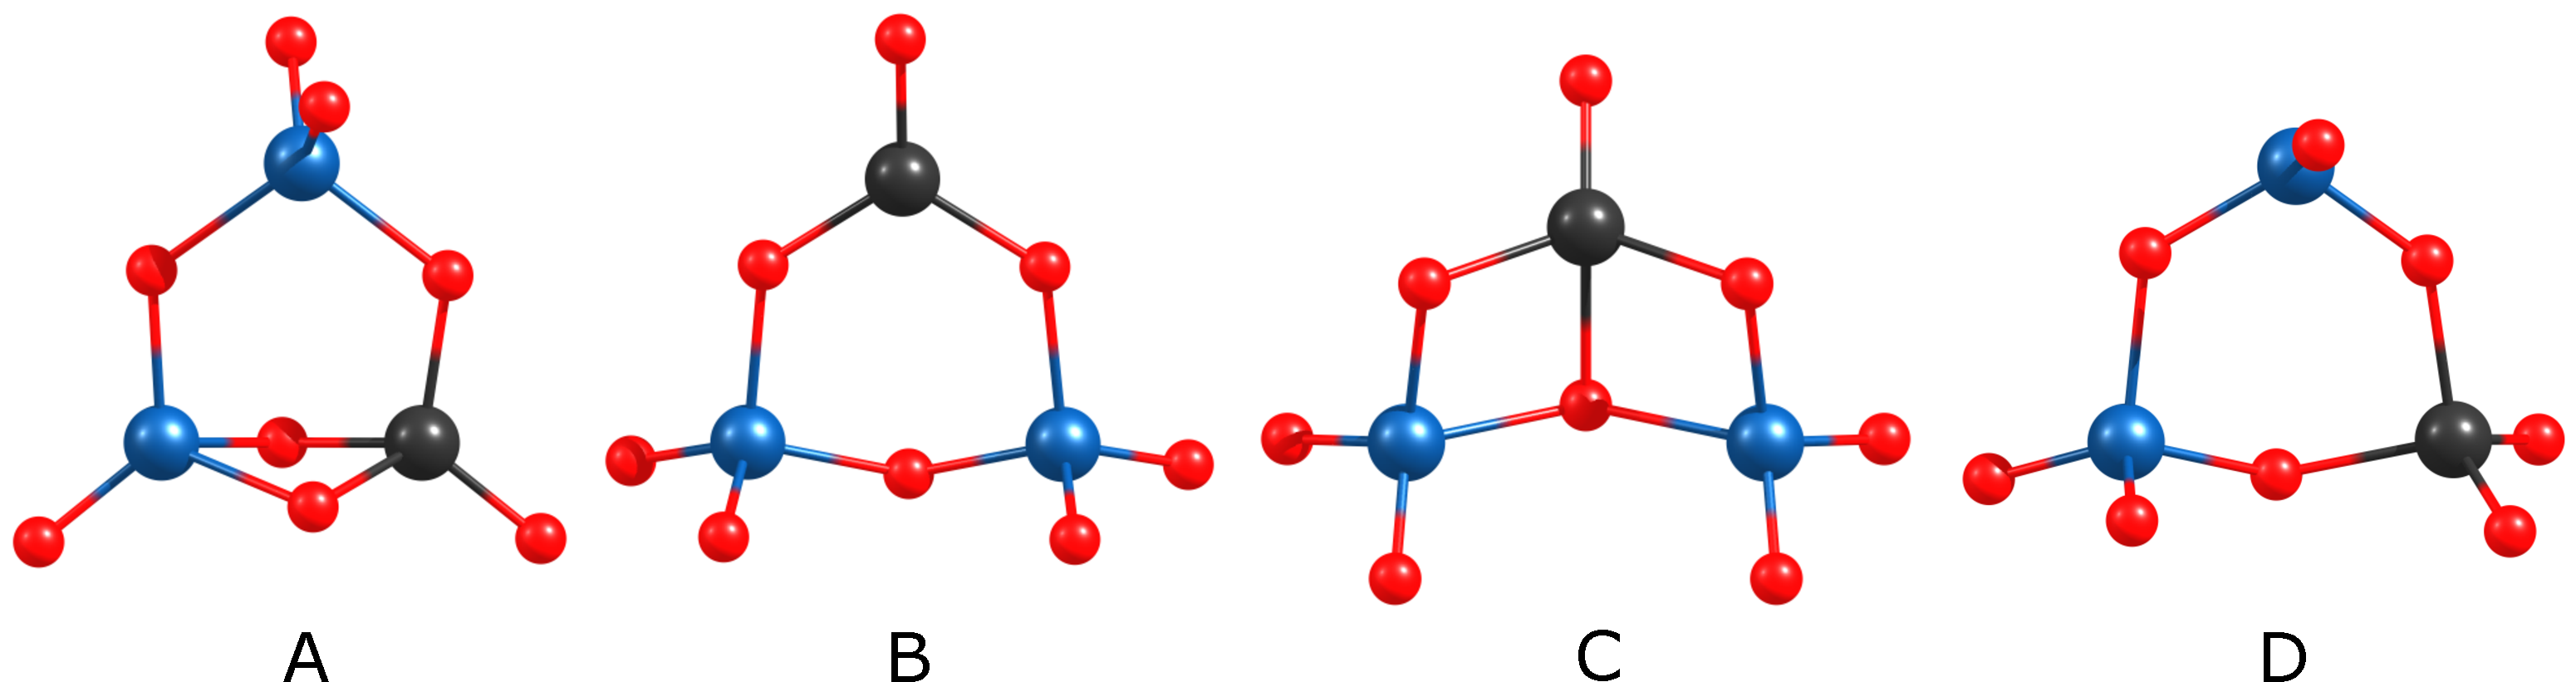
\includegraphics[width=0.75\linewidth]{Cr2MnO8-iso}
	\caption{Geometrical structures of the lowest energy isomers of \ch{Cr2MnO8+}. The shown structures are obtained with the TPSS/def2TZVP optimizations. Chromium, manganese, and oxygen atoms are represented as blue, black, and red spheres, respectively.}
	\label{figs:Cr2MnO8}
\end{figure}





\begin{table}[]
	\centering
	\caption{Relative energies (in eV) of the low energy isomers of \ch{Cr2MnO9+} calculated at the TPSS level}
	\begin{tabular}{@{}lllc@{}}
	\toprule
	state & isomer & sym. & relative energy (eV) \\ \midrule
	$^1$A    & A      & C1   & 0.00                 \\
	$^3$A    & A      & C1   & 0.87                 \\
	$^5$A    & A      & C1   & 2.26                 \\ \bottomrule
	\end{tabular}
\end{table}



\begin{figure}
	\centering
	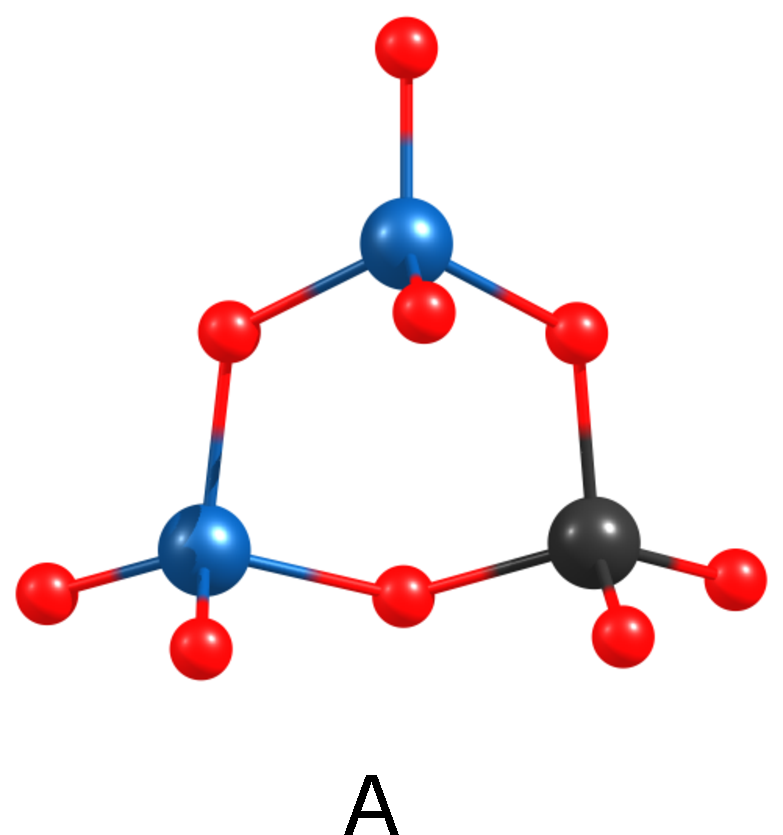
\includegraphics[scale=0.18]{Cr2MnO9-iso}
	\caption{Geometrical structures of the lowest energy isomer of \ch{Cr2MnO9+}. The shown structures are obtained with the TPSS/def2TZVP optimizations. Chromium, manganese, and oxygen atoms are represented as blue, black, and red spheres, respectively.}
	\label{figs:Cr2MnO8}
\end{figure}








\begin{table}[]
	\centering
	\caption{Relative energies (in eV) of the low energy isomers of \ch{Cr2Mn2O5+} calculated at the TPSS level}
	\begin{tabular}{@{}lllc@{}}
	\toprule
	state & isomer & sym. & relative energy (eV) \\ \midrule
	$^8$A      & A      & C$_1$   & 0.00                 \\
	$^4$A      & A      & C$_1$   & 0.10                 \\
	$^{10}$A   & A      & C$_1$   & 0.14                 \\
	$^2$A      & A      & C$_1$   & 0.20                 \\
	$^6$A      & A      & C$_1$   & 0.39                 \\
	$^{12}$A   & A      & C$_1$   & 0.41                 \\
	$^6$A      & B      & C$_1$   & 0.75                 \\
	$^{12}$A   & B      & C$_1$   & 0.77                 \\
	$^4$A      & C      & C$_1$   & 0.94                 \\
	$^6$A      & D      & C$_1$   & 0.94                 \\ \bottomrule
	\end{tabular}
\end{table}



\begin{figure}
	\centering
	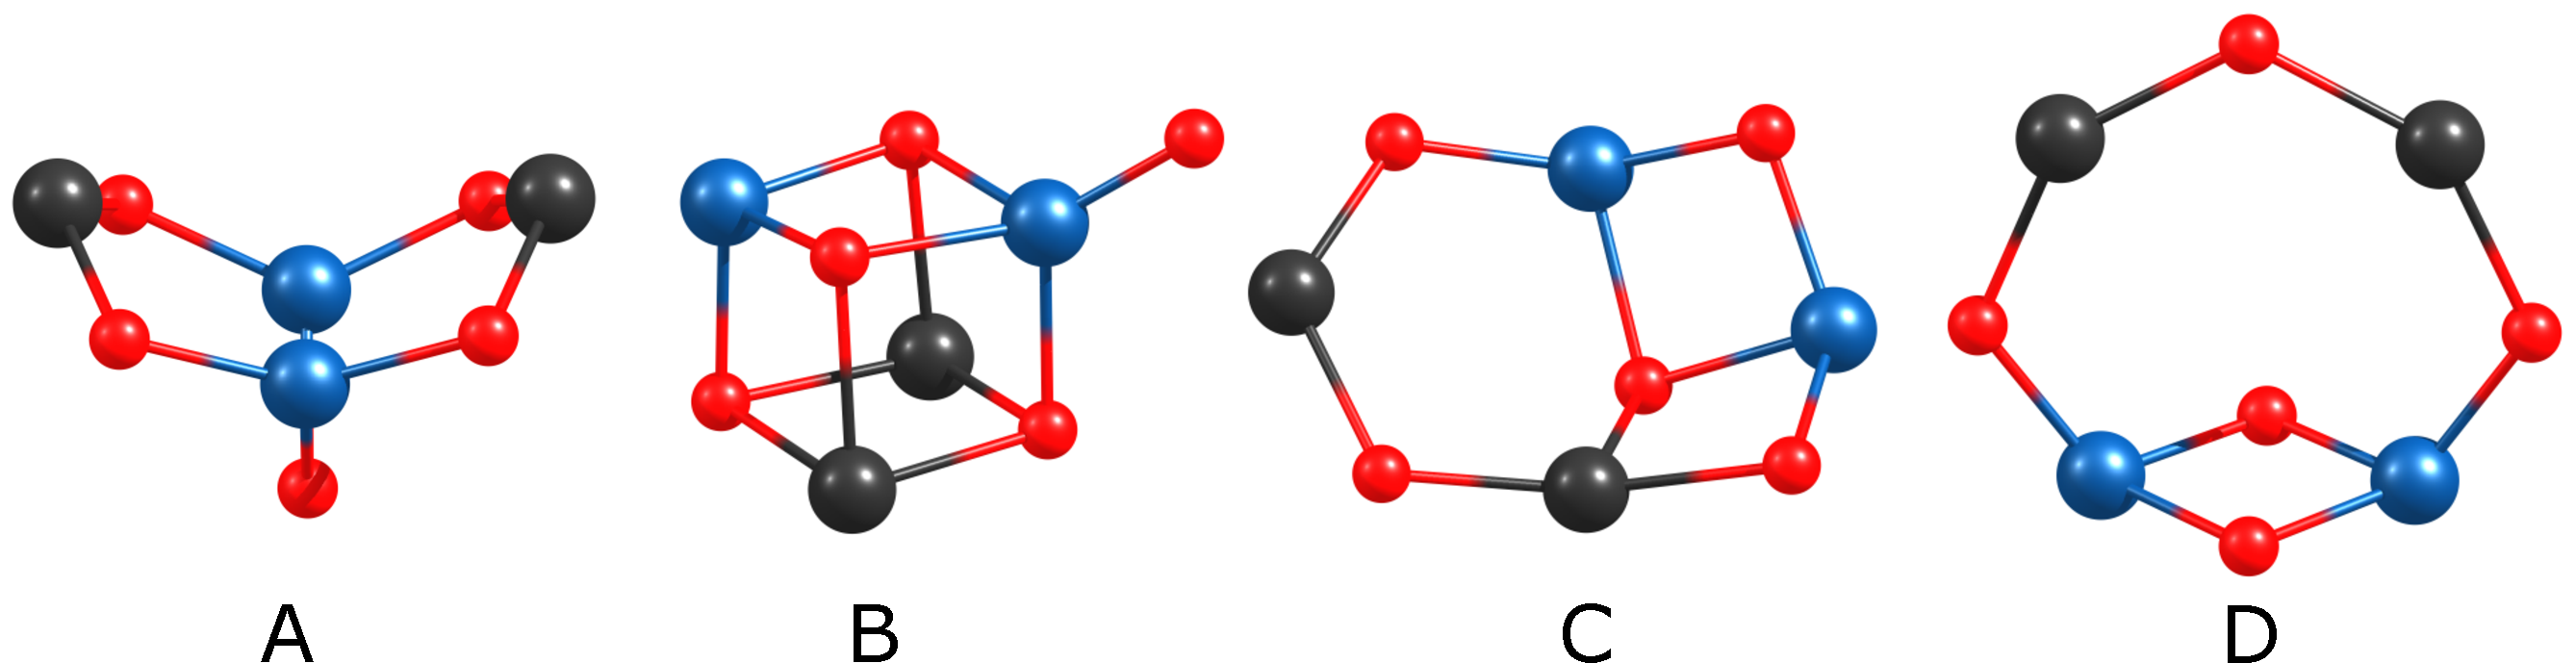
\includegraphics[width=0.60\linewidth]{Cr2Mn2O5-iso}
	\caption{Geometrical structures of the lowest energy isomers of \ch{Cr2Mn2O5+}. The shown structures are obtained with the TPSS/def2TZVP optimizations. Chromium, manganese, and oxygen atoms are represented as blue, black, and red spheres, respectively.}
	\label{figs:Cr2Mn2O5}
\end{figure}







\begin{table}[]
	\centering
	\caption{Relative energies (in eV) of the low energy isomers of \ch{CrMn3O5+} calculated at the TPSS level}
	\begin{tabular}{@{}lllc@{}}
	\toprule
	state & isomer & sym. & relative energy (eV) \\ \midrule
	$^7$A      & A      & C$_1$   & 0.00                 \\
	$^{11}$A   & A      & C$_1$   & 0.03                 \\
	$^5$A      & A      & C$_1$   & 0.19                 \\
	$^{13}$A   & A      & C$_1$   & 0.30                 \\
	$^{17}$A   & A      & C$_1$   & 0.31                 \\
	$^7$A      & B      & C$_1$   & 0.35                 \\
	$^5$A      & B      & C$_1$   & 0.46                 \\
	$^{17}$A   & A      & C$_1$   & 0.36                 \\
	$^1$A      & A      & C$_1$   & 0.45                 \\
	$^3$A      & A      & C$_1$   & 0.47                 \\
	$^3$A      & C      & C$_1$   & 0.66                 \\
	$^{15}$A   & B      & C$_1$   & 0.69                 \\
	$^{11}$A   & D      & C$_1$   & 0.71                 \\
	$^{17}$A   & B      & C$_1$   & 0.76                 \\ \bottomrule
	\end{tabular}
\end{table}



\begin{figure}
	\centering
	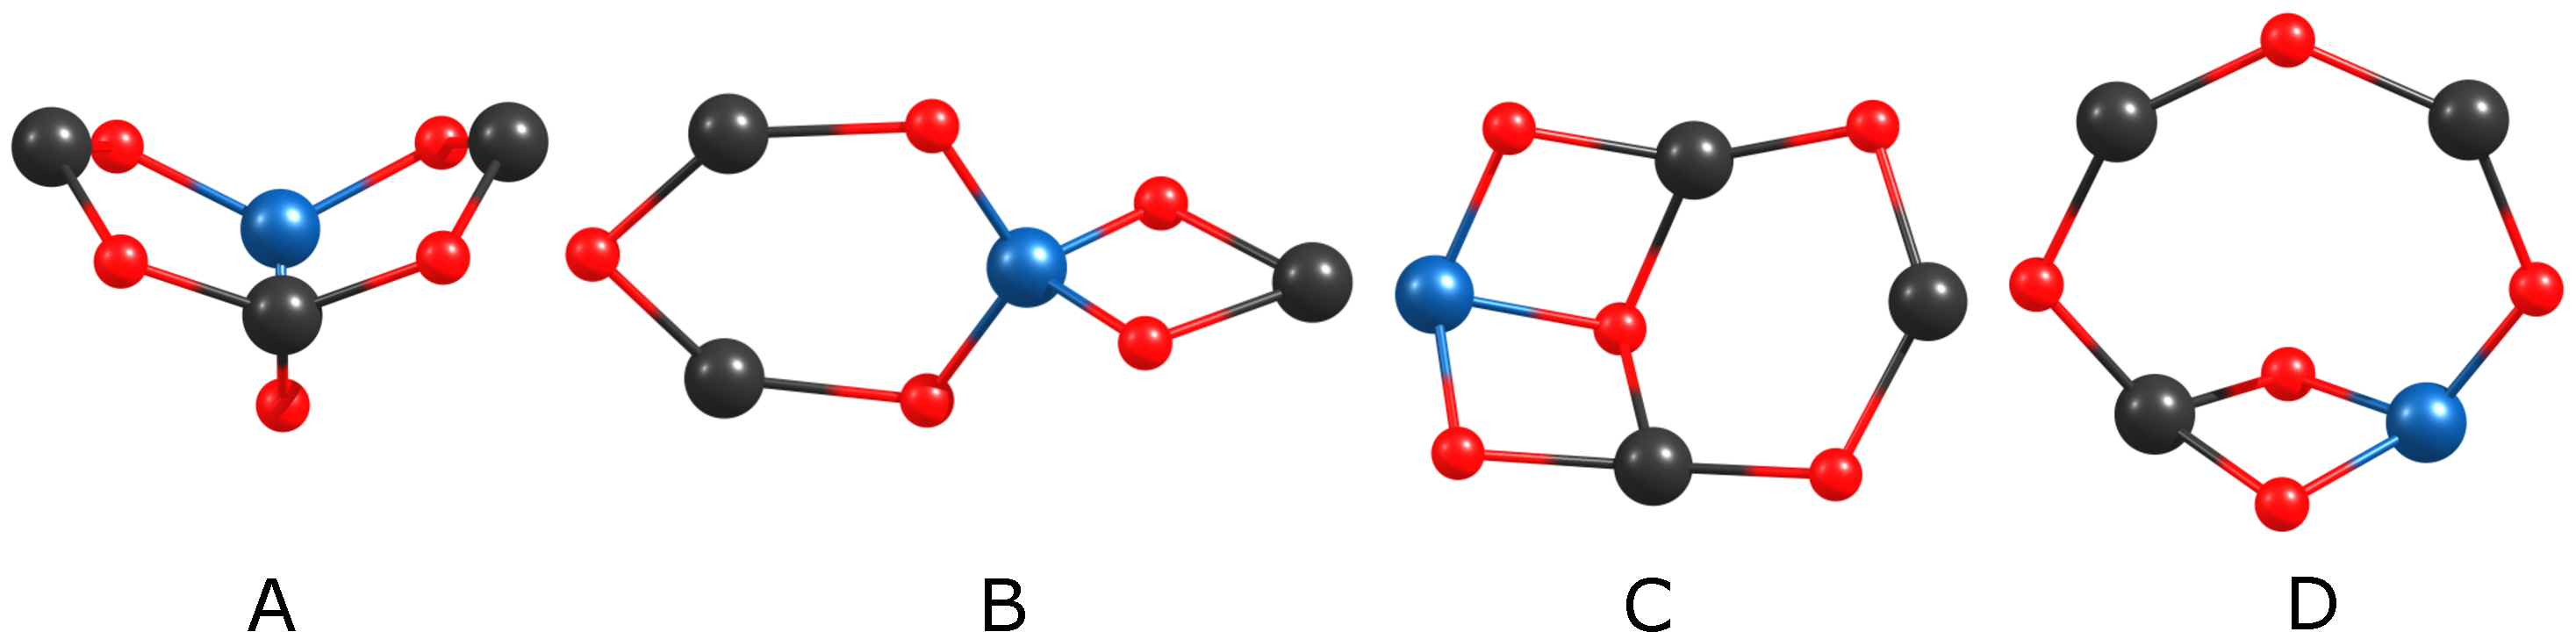
\includegraphics[width=0.7\linewidth]{CrMn3O5-iso}
	\caption{Geometrical structures of the lowest energy isomers of \ch{CrMn3O5+}. The shown structures are obtained with the TPSS/def2TZVP optimizations. Chromium, manganese, and oxygen atoms are represented as blue, black, and red spheres, respectively.}
	\label{figs:CrMn3O5}
\end{figure}






\FloatBarrier



\begin{table}[]
	\centering
	\caption{Relative energies (in eV) of the low energy isomers of \ch{Cr3MnO5+} calculated at the TPSS level}
	\begin{tabular}{@{}lllc@{}}
	\toprule
	state & isomer & sym. & relative energy (eV) \\ \midrule
	$^7$A     & A      & C$_1$   & 0.00                 \\
	$^9$A     & A      & C$_1$   & 0.19                 \\
	$^3$A     & A      & C$_1$   & 0.23                 \\
	$^3$A     & B      & C$_1$   & 0.28                 \\
	$^{11}$A  & A      & C$_1$   & 0.35                 \\
	$^9$A     & C      & C$_1$   & 0.35                 \\
	$^9$A     & B      & C$_1$   & 0.41                 \\
	$^{15}$A  & C      & C$_1$   & 0.42                 \\
	$^{15}$A  & B      & C$_1$   & 0.47                 \\
	$^{15}$A  & A      & C$_1$   & 0.53                 \\
	$^{15}$A  & A      & C$_1$   & 0.54                 \\
	$^{15}$A  & D      & C$_1$   & 0.76                 \\ \bottomrule
	\end{tabular}
\end{table}




\begin{figure}
	\centering
	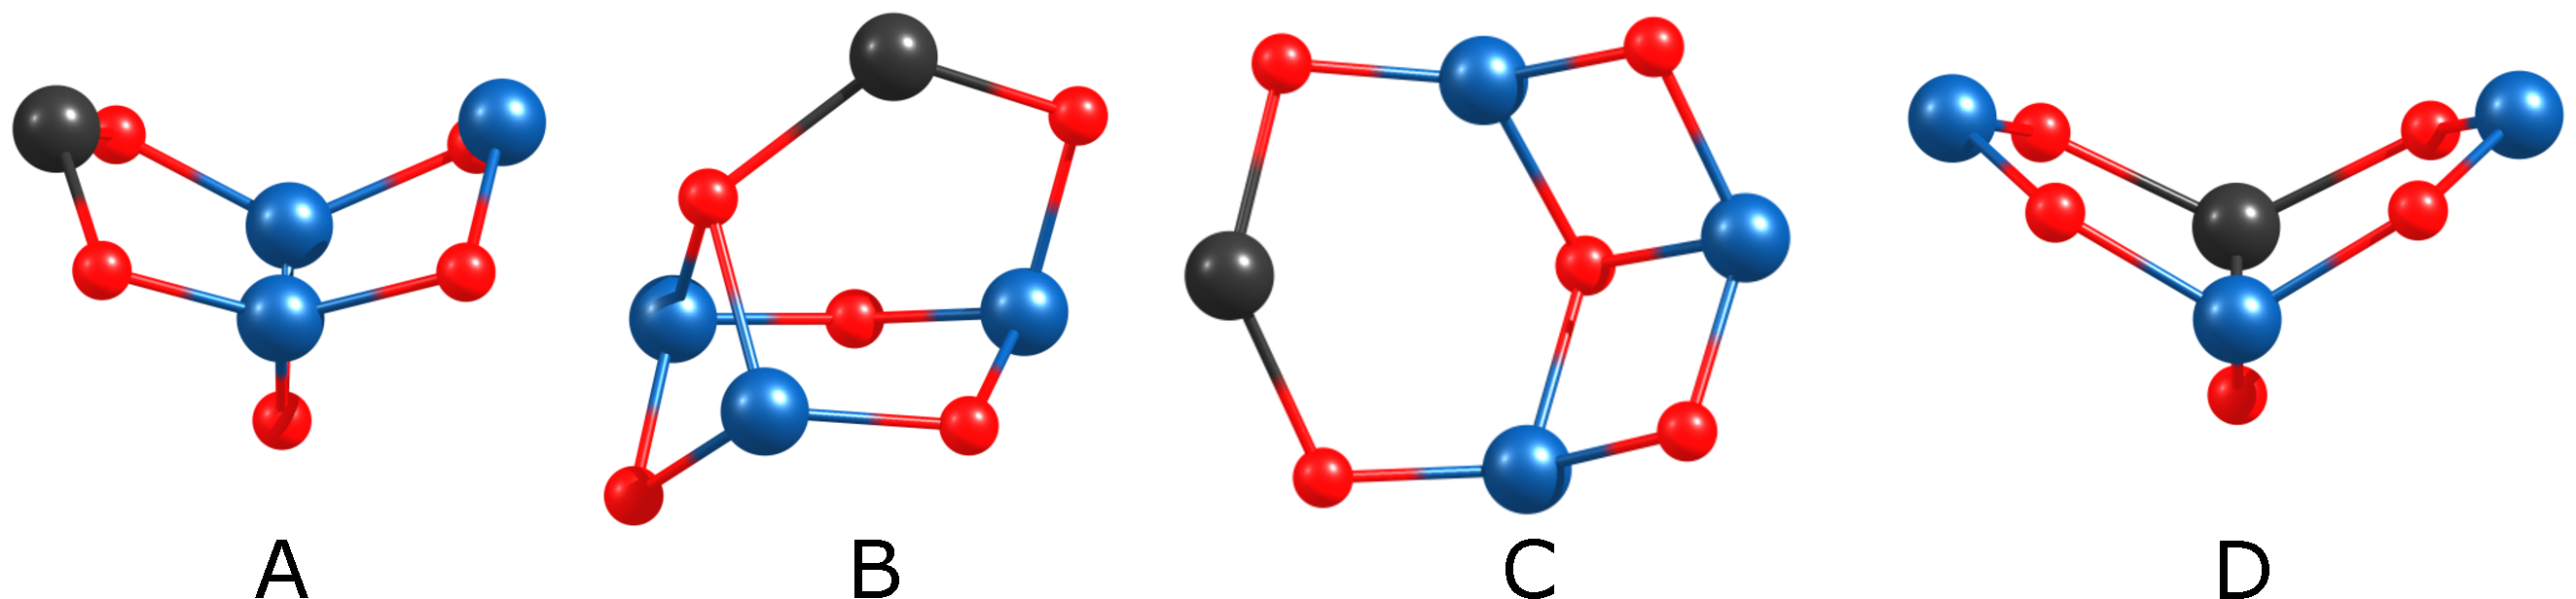
\includegraphics[width=0.6\linewidth]{Cr3MnO5-iso}
	\caption{Geometrical structures of the lowest energy isomers of \ch{Cr3MnO5+}. The shown structures are obtained with the TPSS/def2TZVP optimizations. Chromium, manganese, and oxygen atoms are represented as blue, black, and red spheres, respectively.}
	\label{figs:Cr3MnO5}
\end{figure}






\begin{table}[]
	\centering
	\caption{Relative energies (in eV) of the low energy isomers of \ch{Cr2Mn2O6+} calculated at the TPSS level}
	\begin{tabular}{@{}lllc@{}}
	\toprule
	state & isomer & sym. & relative energy (eV) \\ \midrule
	$^8$A      & A      & C$_1$   & 0.00                 \\
	$^4$A      & B      & C$_1$   & 0.06                 \\
	$^6$A      & B      & C$_1$   & 0.12                 \\
	$^8$A      & B      & C$_1$   & 0.12                 \\
	$^2$A      & B      & C$_1$   & 0.22                 \\
	$^{10}$A   & A      & C$_1$   & 0.38                 \\
	$^{10}$A   & B      & C$_1$   & 0.40                 \\
	$^2$A      & A      & C$_1$   & 0.53                 \\
	$^6$A      & A      & C$_1$   & 0.62                 \\ \bottomrule
	\end{tabular}
\end{table}



\begin{figure}
	\centering
	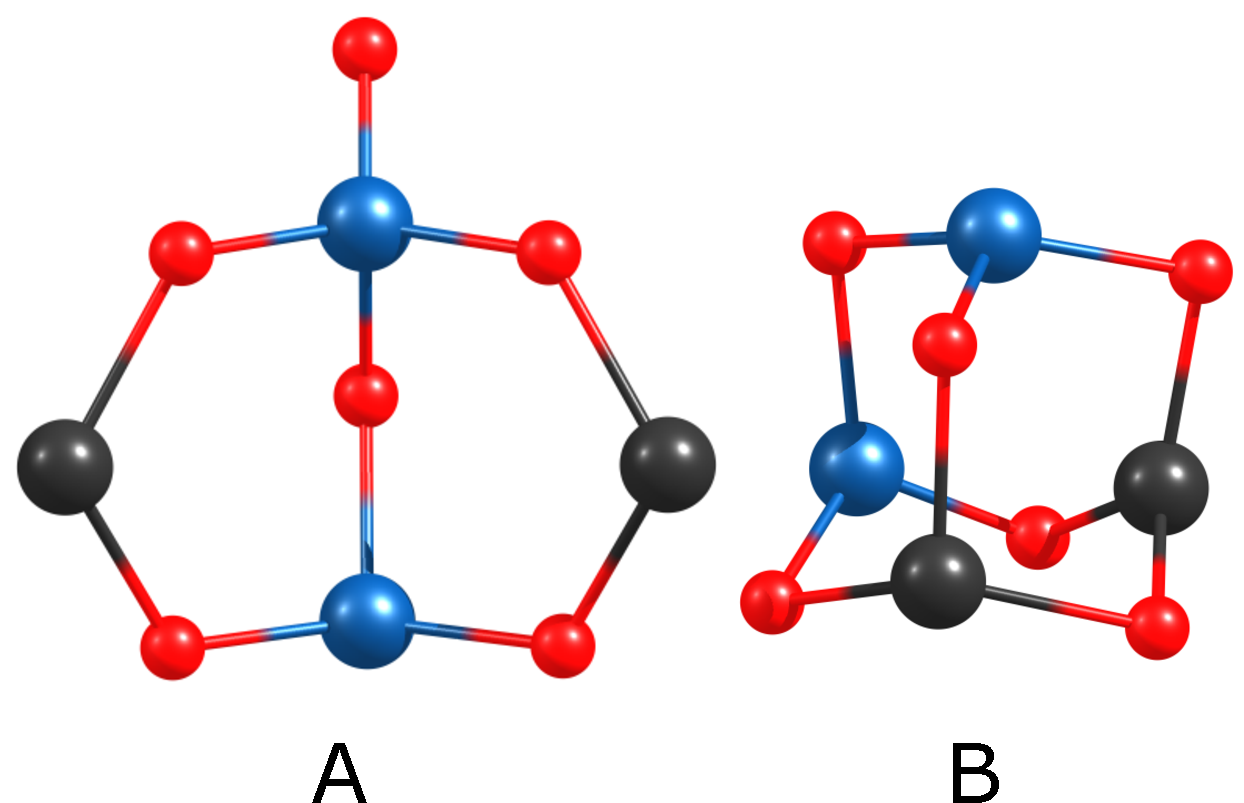
\includegraphics[scale=0.17]{Cr2Mn2O6-iso}
	\caption{Geometrical structures of the lowest energy isomers of \ch{Cr2Mn2O6+}. The shown structures are obtained with the TPSS/def2TZVP optimizations. Chromium, manganese, and oxygen atoms are represented as blue, black, and red spheres, respectively.}
	\label{figs:Cr2Mn2O6}
\end{figure}









\begin{table}[]
	\centering
	\caption{Relative energies (in eV) of the low energy isomers of \ch{Cr3MnO6+} calculated at the TPSS level}
	\begin{tabular}{@{}lllc@{}}
	\toprule
	state & isomer & sym. & relative energy (eV) \\ \midrule
	$^{11}$A   & A      & C$_1$   & 0.00                 \\
	$^7$A      & A      & C$_1$   & 0.03                 \\
	$^5$A      & A      & C$_1$   & 0.03                 \\
	$^9$A      & A      & C$_1$   & 0.05                 \\
	$^3$A      & A      & C$_1$   & 0.17                 \\
	$^7$A      & B      & C$_1$   & 0.90                 \\ \bottomrule
	\end{tabular}
\end{table}


\begin{figure}
	\centering
	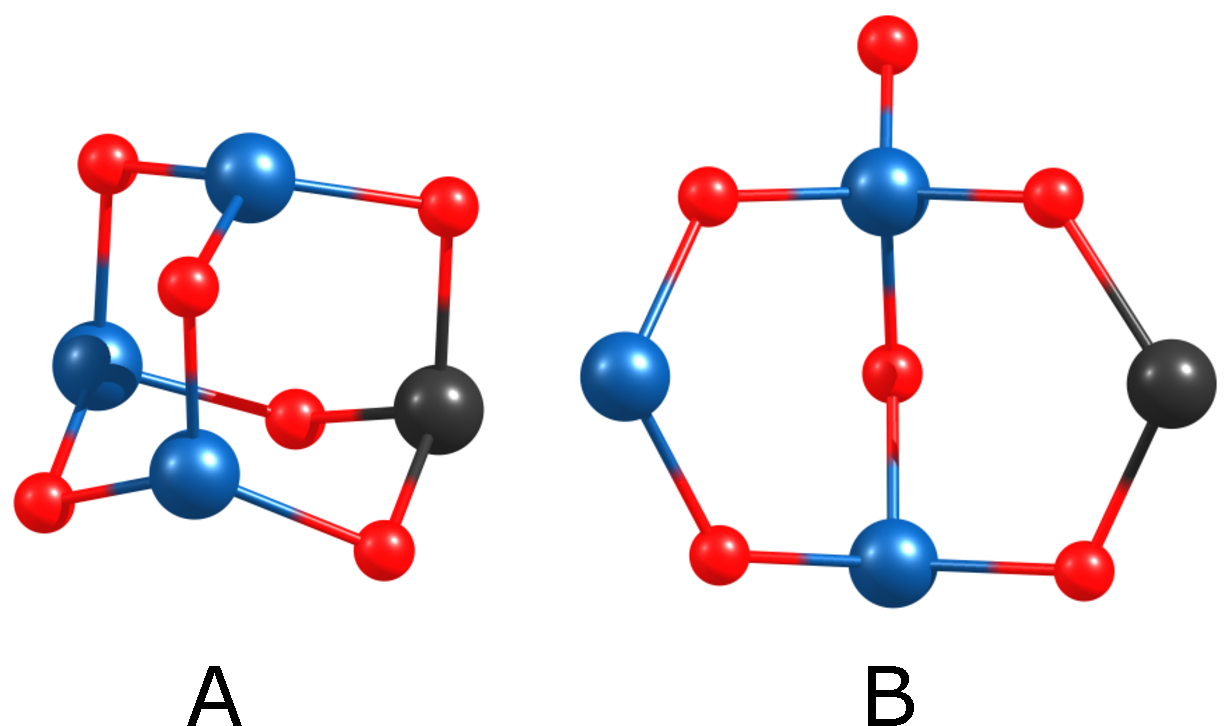
\includegraphics[scale=0.19]{Cr3MnO6-iso}
	\caption{Geometrical structures of the lowest energy isomers of \ch{Cr3MnO6+}. The shown structures are obtained with the TPSS/def2TZVP optimizations. Chromium, manganese, and oxygen atoms are represented as blue, black, and red spheres, respectively.}
	\label{figs:Cr3MnO6}
\end{figure}








\begin{table}[]
	\centering
	\caption{Relative energies (in eV) of the low energy isomers of \ch{Cr3MnO7+} calculated at the TPSS level}
	\begin{tabular}{@{}lllc@{}}
	\toprule
	state & isomer & sym. & relative energy (eV) \\ \midrule
	$^5$A    & A      & C$_1$   & 0.00                 \\
	$^7$A    & A      & C$_1$   & 0.16                 \\
	$^3$A    & A      & C$_1$   & 0.17                 \\
	$^1$A    & A      & C$_1$   & 0.20                 \\
	$^9$A    & A      & C$_1$   & 0.21                 \\
	$^7$A    & B      & C$_1$   & 0.61                 \\ \bottomrule
	\end{tabular}
\end{table}


\FloatBarrier

\begin{figure}
	\centering
	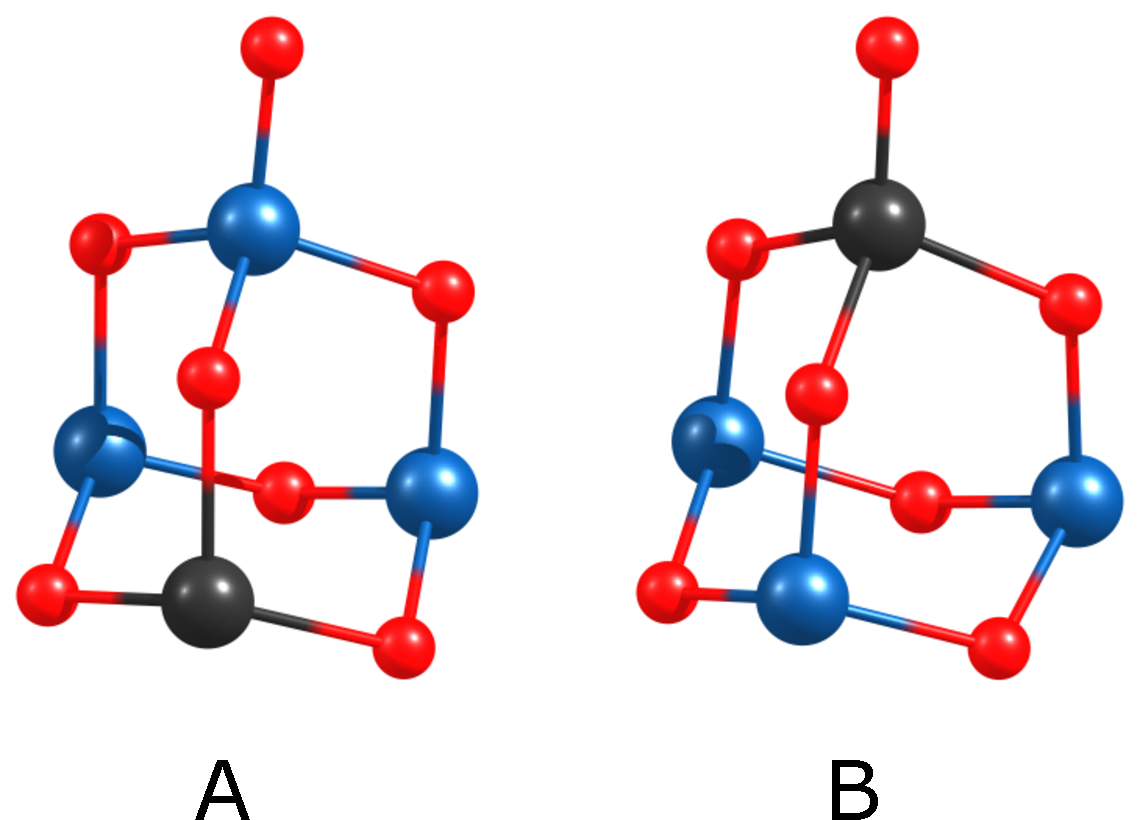
\includegraphics[scale=0.18]{Cr3MnO7-iso}
	\caption{Geometrical structures of the lowest energy isomers of \ch{Cr3MnO7+}. The shown structures are obtained with the TPSS/def2TZVP optimizations. Chromium, manganese, and oxygen atoms are represented as blue, black, and red spheres, respectively.}
	\label{figs:Cr3MnO7}
\end{figure}







\begin{table}[]
	\centering
	\caption{Relative energies (in eV) of the low energy isomers of \ch{CrMn3O8+} calculated at the TPSS level}
	\begin{tabular}{@{}lllc@{}}
	\toprule
	state & isomer & sym. & relative energy (eV) \\ \midrule
	$^5$A      & A      & C$_1$   & 0.00                 \\
	$^7$A      & A      & C$_1$   & 0.06                 \\
	$^3$A      & A      & C$_1$   & 0.19                 \\
	$^9$A      & A      & C$_1$   & 0.45                 \\
	$^{11}$A   & A      & C$_1$   & 0.60                 \\
	$^5$A      & B      & C$_1$   & 0.77                 \\ \bottomrule
	\end{tabular}
\end{table}



\begin{figure}
	\centering
	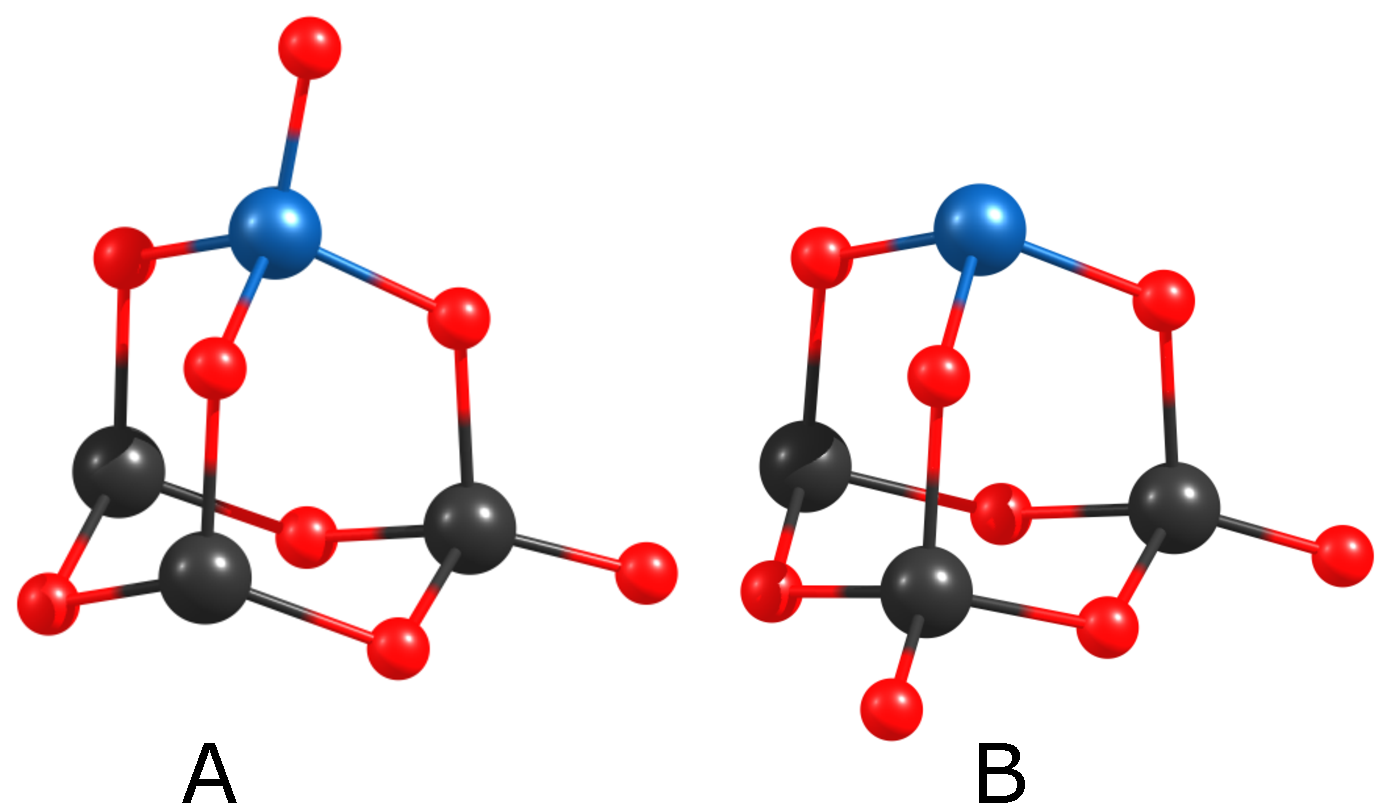
\includegraphics[scale=0.18]{CrMn3O8-iso}
	\caption{Geometrical structures of the lowest energy isomers of \ch{CrMn3O8+}. The shown structures are obtained with the TPSS/def2TZVP optimizations. Chromium, manganese, and oxygen atoms are represented as blue, black, and red spheres, respectively.}
	\label{figs:CrMn3O8}
\end{figure}








\begin{table}[]
	\centering
	\caption{Relative energies (in eV) of the low energy isomers of \ch{CrMn3O9+} calculated at the TPSS level}
	\begin{tabular}{@{}lllc@{}}
	\toprule
	state & isomer & sym. & relative energy (eV) \\ \midrule
	$^3$A    & A      & C$_1$   & 0.00                 \\
	$^5$A    & A      & C$_1$   & 0.15                 \\
	$^7$A    & A      & C$_1$   & 0.66                 \\
	$^3$A    & B      & C$_1$   & 1.09                 \\ \bottomrule
	\end{tabular}
\end{table}


\begin{figure}
	\centering
	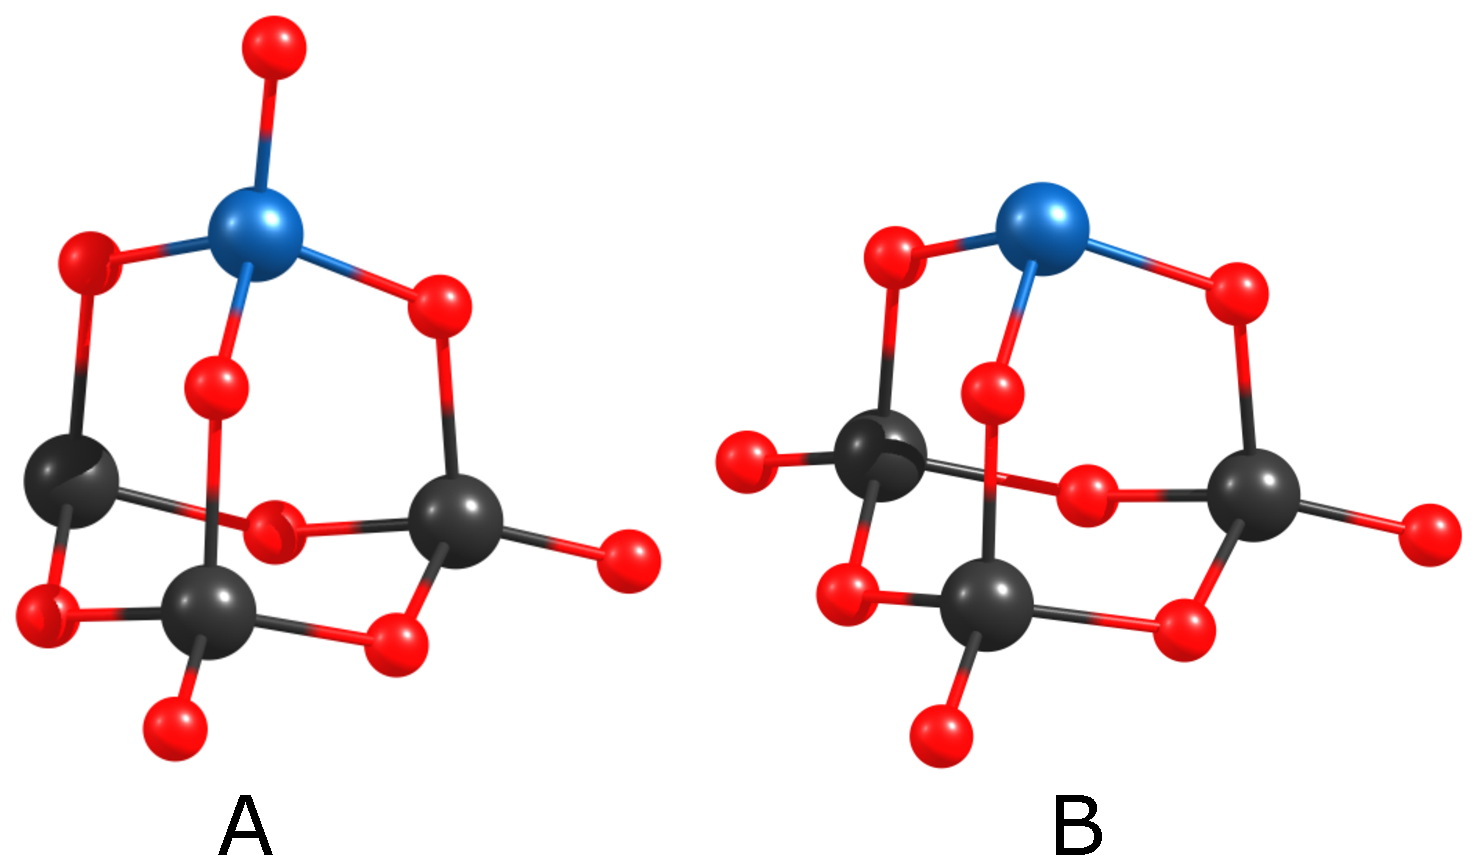
\includegraphics[scale=0.18]{CrMn3O9-iso}
	\caption{Geometrical structures of the lowest energy isomers of \ch{CrMn3O9+}. The shown structures are obtained with the TPSS/def2TZVP optimizations. Chromium, manganese, and oxygen atoms are represented as blue, black, and red spheres, respectively.}
	\label{figs:CrMn3O9}
\end{figure}






\begin{table}[]
	\centering
	\caption{Relative energies (in eV) of the low energy isomers of \ch{Cr2Mn2O9+} calculated at the TPSS level}
	\begin{tabular}{@{}lllc@{}}
	\toprule
	   state & isomer & sym.    & relative energy (eV) \\ \midrule
	$^4$A    & A      & C$_1$   & 0.00                 \\
	$^6$A    & A      & C$_1$   & 0.51                 \\
	$^2$A    & A      & C$_1$   & 0.70                 \\
	$^8$A    & A      & C$_1$   & 0.74                 \\
	$^4$A    & B      & C$_1$   & 1.14                 \\ \bottomrule
	\end{tabular}
\end{table}


\begin{figure}
	\centering
	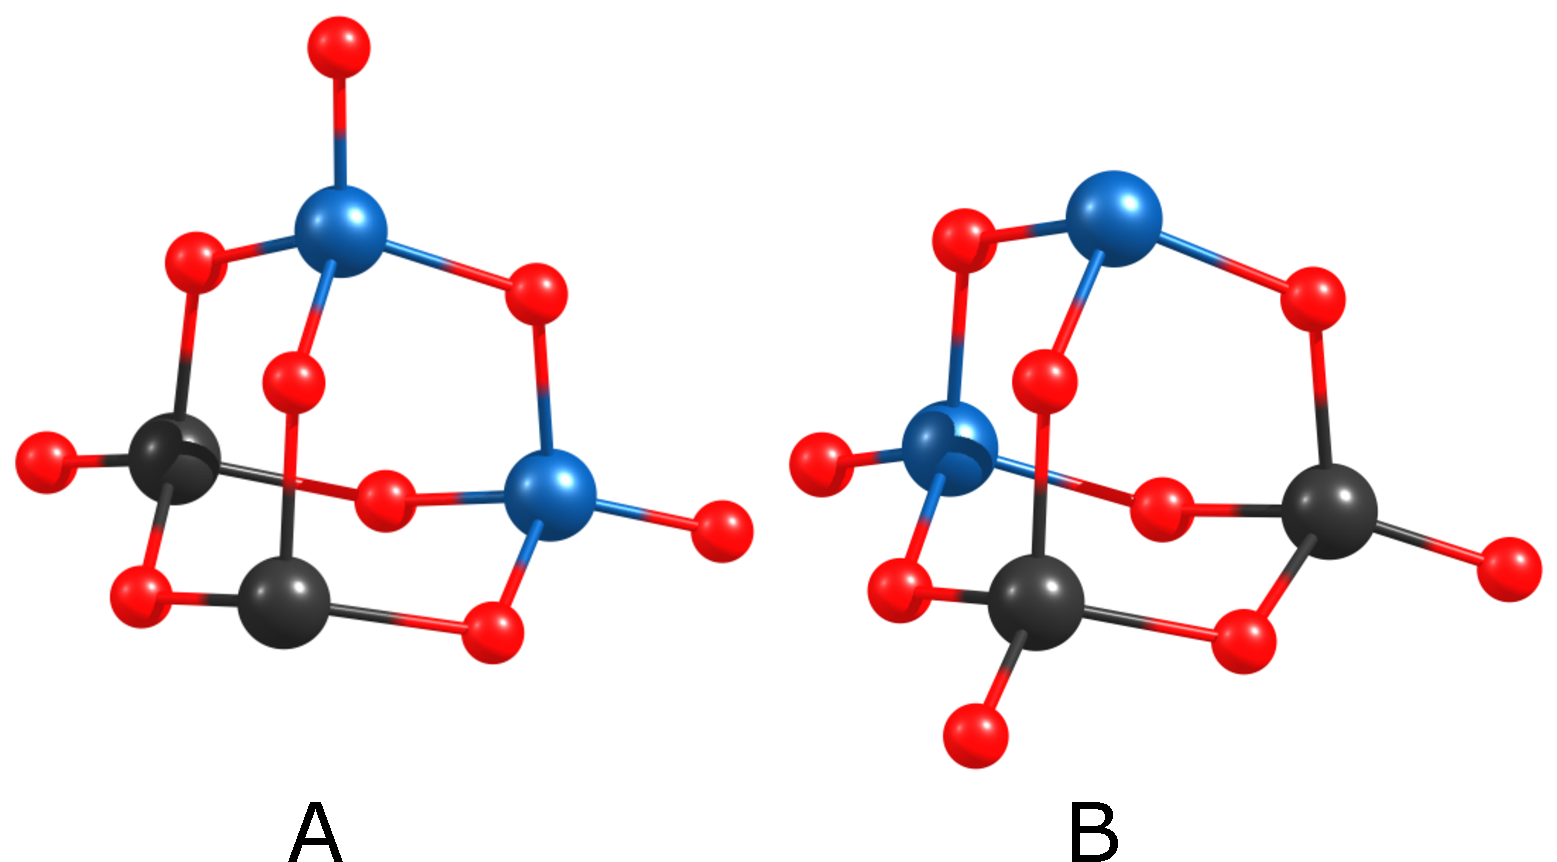
\includegraphics[scale=0.16]{Cr2Mn2O9-iso}
	\caption{Geometrical structures of the lowest energy isomers of \ch{Cr2Mn2O9+}. The shown structures are obtained with the TPSS/def2TZVP optimizations. Chromium, manganese, and oxygen atoms are represented as blue, black, and red spheres, respectively.}
	\label{figs:Cr2Mn2O9}
\end{figure}




\FloatBarrier



\begin{table}[]
	\centering
	\caption{Relative energies (in eV) of the low energy isomer of \ch{Cr3MnO10+} calculated at the TPSS level}
	\begin{tabular}{@{}llc@{}}
	\toprule
	   state & sym. & relative energy (eV) \\ \midrule
	$^1$A    & C$_1$   & 0.00                 \\
	$^3$A    & C$_1$   & 0.48                 \\
	$^5$A    & C$_1$   & 0.92                 \\ \bottomrule
	\end{tabular}
\end{table}


\begin{table}[]
	\centering
	\caption{Relative energies (in eV) of the low energy isomer of \ch{Cr2Mn2O10+} calculated at the TPSS level}
	\begin{tabular}{@{}llc@{}}
	\toprule
	   state & sym.    & relative energy (eV) \\ \midrule
	$^2$A    & C$_1$   & 0.00                 \\
	$^4$A    & C$_1$   & 0.51                 \\
	$^6$A    & C$_1$   & 1.01                 \\ \bottomrule
	\end{tabular}
\end{table}



\begin{table}[]
	\centering
	\caption{Relative energies (in eV) of the low energy isomer of \ch{CrMn3O10+} calculated at the TPSS level}
	\begin{tabular}{@{}llc@{}}
	\toprule
	state & sym. & relative energy (eV) \\ \midrule
	$^3$A    & C$_1$   & 0.00                 \\
	$^1$A    & C$_1$   & 0.26                 \\
	$^5$A    & C$_1$   & 0.46                 \\
	$^7$A    & C$_1$   & 0.93                 \\ \bottomrule
	\end{tabular}
\end{table}






\begin{figure}
	\centering
	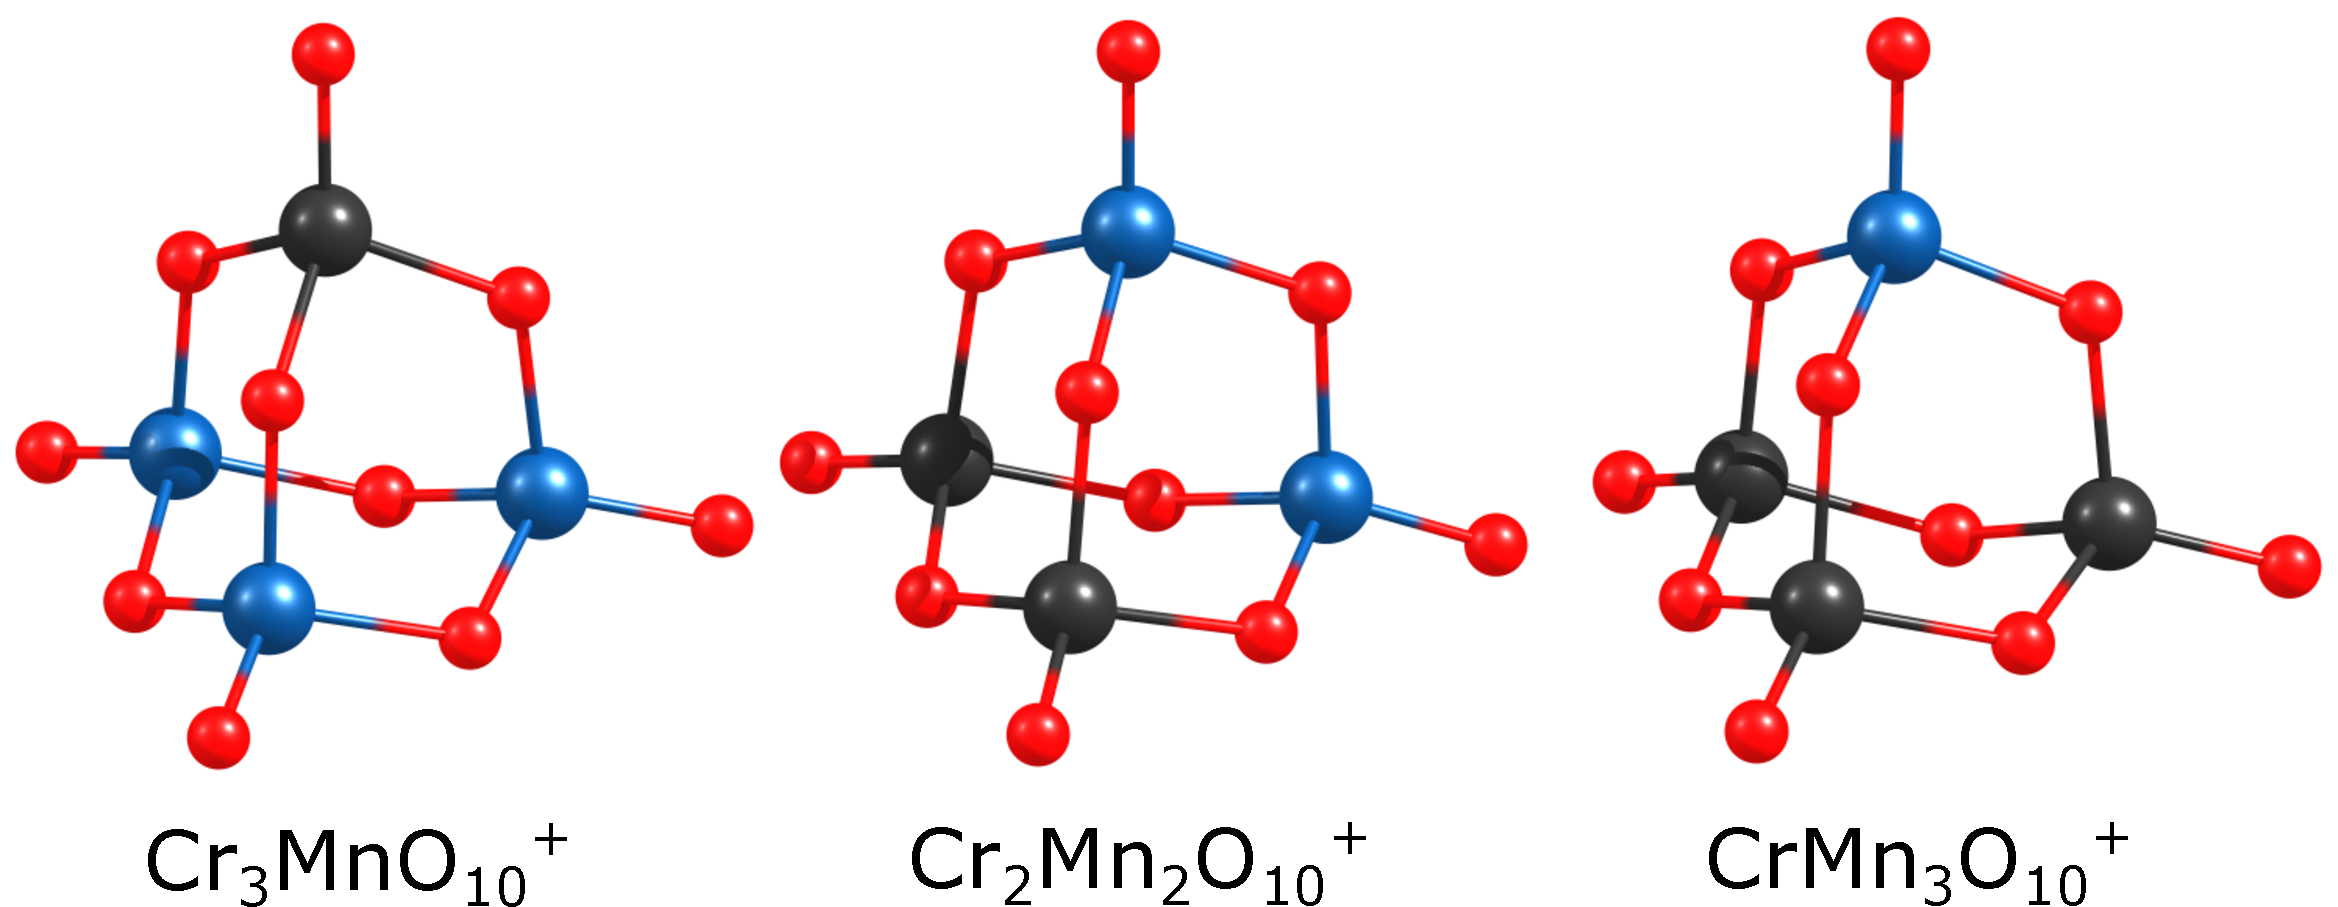
\includegraphics[scale=0.16]{CrxMnyO10-iso}
	\caption{Geometrical structures of the lowest energy isomers of \ch{Cr3MnO10+}, \ch{Cr2Mn2O10+}, and \ch{CrMn3O10+}. The shown structures are obtained with the TPSS/def2TZVP optimizations. Chromium, manganese, and oxygen atoms are represented as blue, black, and red spheres, respectively.}
	\label{figs:CrxMnyO10}
\end{figure}


\newpage


\begin{table}[]
	\centering
	\caption{Relative energies (in eV) of the low energy isomers of \ch{Cr3MnO11+} calculated at the TPSS level}
	\begin{tabular}{@{}lllc@{}}
	\toprule
	   state & isomer & sym.    & relative energy (eV) \\ \midrule
	$^3$A    & A      & C$_1$   & 0.00                 \\
	$^3$A    & B      & C$_1$   & 0.18                 \\
	$^1$A    & B      & C$_1$   & 0.31                 \\
	$^1$A    & C      & C$_1$   & 0.65                 \\
	$^3$A    & D      & C$_1$   & 0.91                 \\ \bottomrule
	\end{tabular}
\end{table}




\begin{figure}
	\centering
	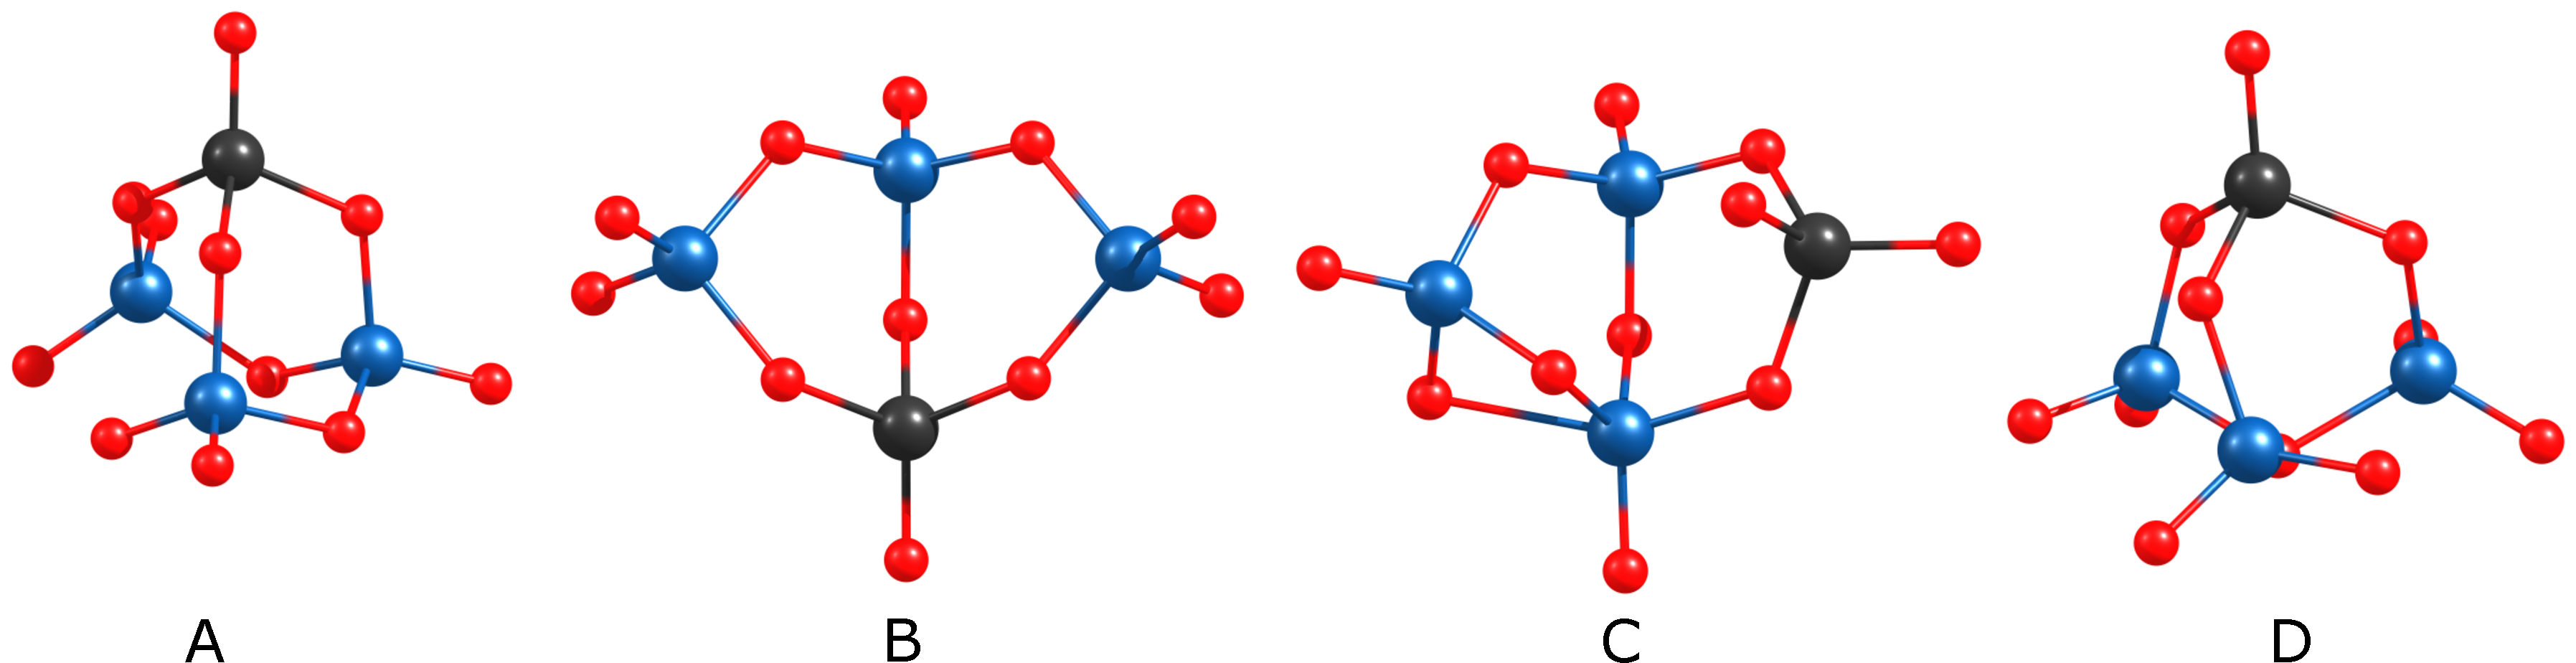
\includegraphics[width=0.8\linewidth]{Cr3MnO11-iso}
	\caption{Geometrical structures of the lowest energy isomers of \ch{Cr3MnO11+}. The shown structures are obtained with the TPSS/def2TZVP optimizations. Chromium, manganese, and oxygen atoms are represented as blue, black, and red spheres, respectively.}
	\label{figs:Cr3MnO11}
\end{figure}







\begin{table}[]
	\centering
	\caption{Relative energies (in eV) of the low energy isomers of \ch{Cr4O5+} calculated at the TPSS level}
	\begin{tabular}{@{}rclc@{}}
	\toprule
	state & isomer & sym. & relative energy (eV) \\ \midrule
	$^4$A      & A      & C$_1$   & 0.00                 \\
	$^{14}$A   & B      & C$_1$   & 0.11                 \\
	$^8$A      & C      & C$_1$   & 0.12                 \\
	$^{14}$A   & A      & C$_1$   & 0.14                 \\
	$^{12}$A   & A      & C$_1$   & 0.16                 \\
	$^{14}$A   & C      & C$_1$   & 0.17                 \\
	$^8$A      & B      & C$_1$   & 0.19                 \\
	$^{14}$A   & A      & C$_1$   & 0.24                 \\
	$^8$A      & A      & C$_1$   & 0.26                 \\
	$^{12}$A     & C      & C$_1$   & 0.33                 \\
	$^2$A      & A      & C$_1$   & 0.34                 \\
	$^6$A      & A      & C$_1$   & 0.43                 \\
	$^{10}$A   & C      & C$_1$   & 0.67                 \\
	$^{10}$A   & B      & C$_1$   & 0.72                 \\ \bottomrule
	\end{tabular}
\end{table}


\begin{figure}
	\centering
	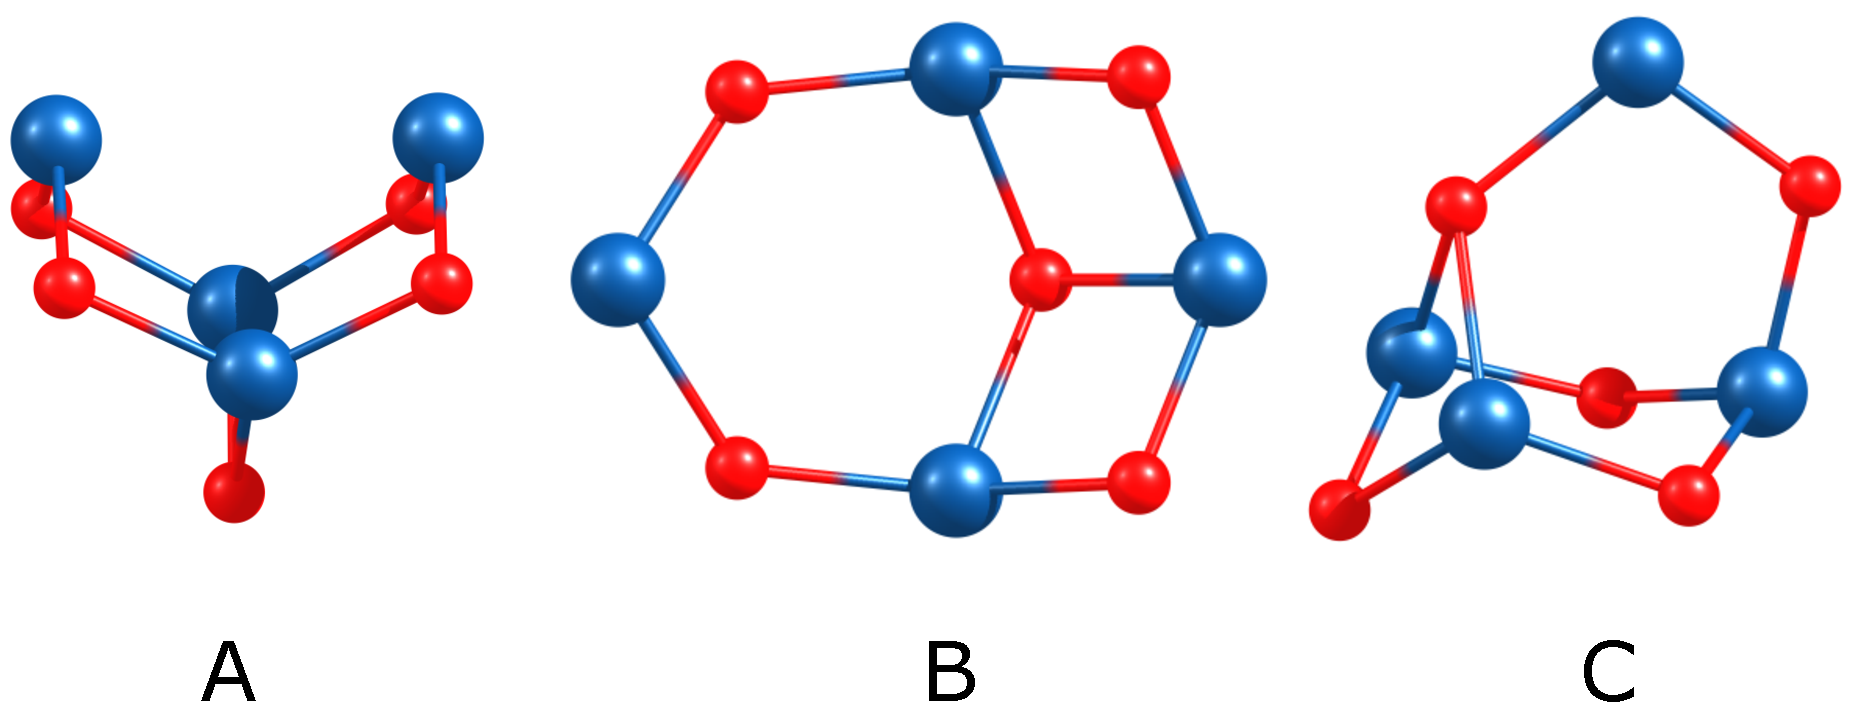
\includegraphics[scale=0.16]{Cr4O5-iso}
	\caption{Geometrical structures of the lowest energy isomers of \ch{Cr4O5+}. The shown structures are obtained with the TPSS/def2TZVP optimizations. Chromium and oxygen atoms are represented as blue and red spheres, respectively.}
	\label{figs:Cr4O5}
\end{figure}


\newpage


\begin{table}[]
	\centering
	\caption{Relative energies (in eV) of the low energy isomers of \ch{Cr4O6+} calculated at the TPSS level}
	\begin{tabular}{@{}rclc@{}}
	\toprule
	state & isomer & sym. & relative energy (eV) \\ \midrule
	$^{10}$A   & A      & C$_1$   & 0.00                 \\
	$^6$A      & A      & C$_1$   & 0.27                 \\
	$^8$A      & A      & C$_1$   & 0.30                 \\
	$^{12}$A   & A      & C$_1$   & 0.36                 \\
	$^{12}$A   & B      & C$_1$   & 1.67                 \\
	$^2$A      & C      & C$_1$   & 1.72                 \\ \bottomrule
	\end{tabular}
\end{table}


\begin{figure}
	\centering
	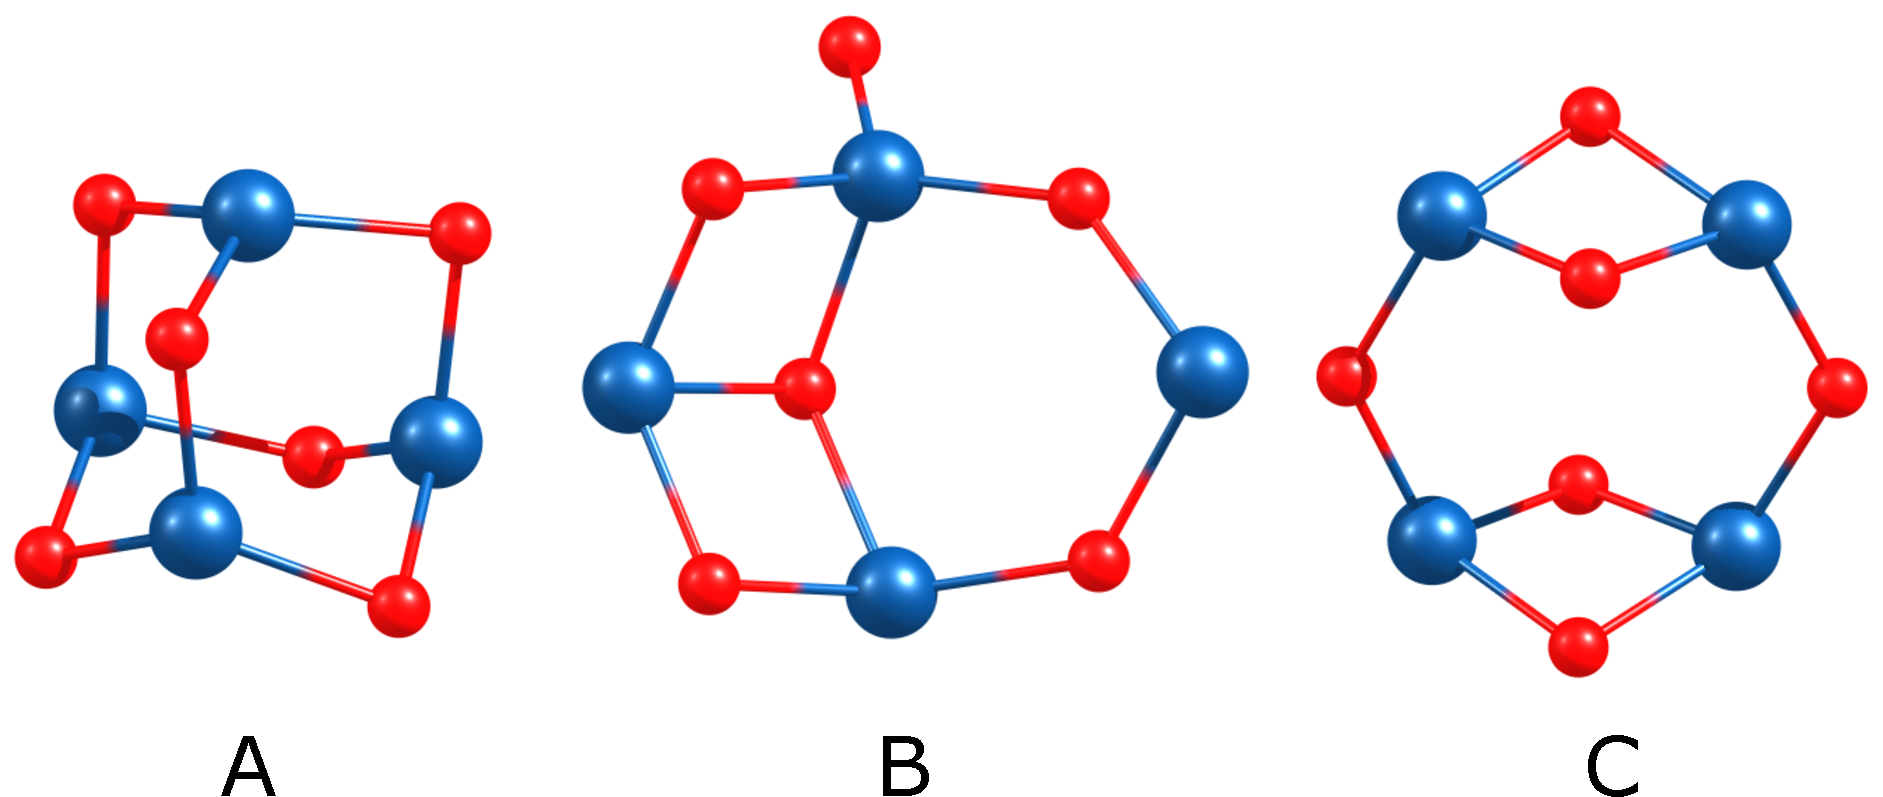
\includegraphics[scale=0.16]{Cr4O6-iso}
	\caption{Geometrical structures of the lowest energy isomers of \ch{Cr4O6+}. The shown structures are obtained with the TPSS/def2TZVP optimizations. Chromium and oxygen atoms are represented as blue and red spheres, respectively.}
	\label{figs:Cr4O6}
\end{figure}




\begin{table}[]
	\centering
	\caption{Relative energies (in eV) of the low energy isomers of \ch{Cr4O7+} calculated at the TPSS level}
	\begin{tabular}{@{}rclc@{}}
	\toprule
		state  & isomer & sym. 	  & relative energy (eV) \\ \midrule
	$^{10}$A   & A      & C$_1$   & 0.00                 \\
	$^4$A      & A      & C$_1$   & 0.10                 \\
	$^8$A      & A      & C$_1$   & 0.12                 \\
	$^6$A      & A      & C$_1$   & 0.15                 \\
	$^2$A      & A      & C$_1$   & 0.38                 \\
	$^{10}$A   & B      & C$_1$   & 1.27                 \\
	$^{10}$A   & C      & C$_1$   & 1.34                 \\ \bottomrule
	\end{tabular}
\end{table}



\clearpage


\begin{figure}
	\centering
	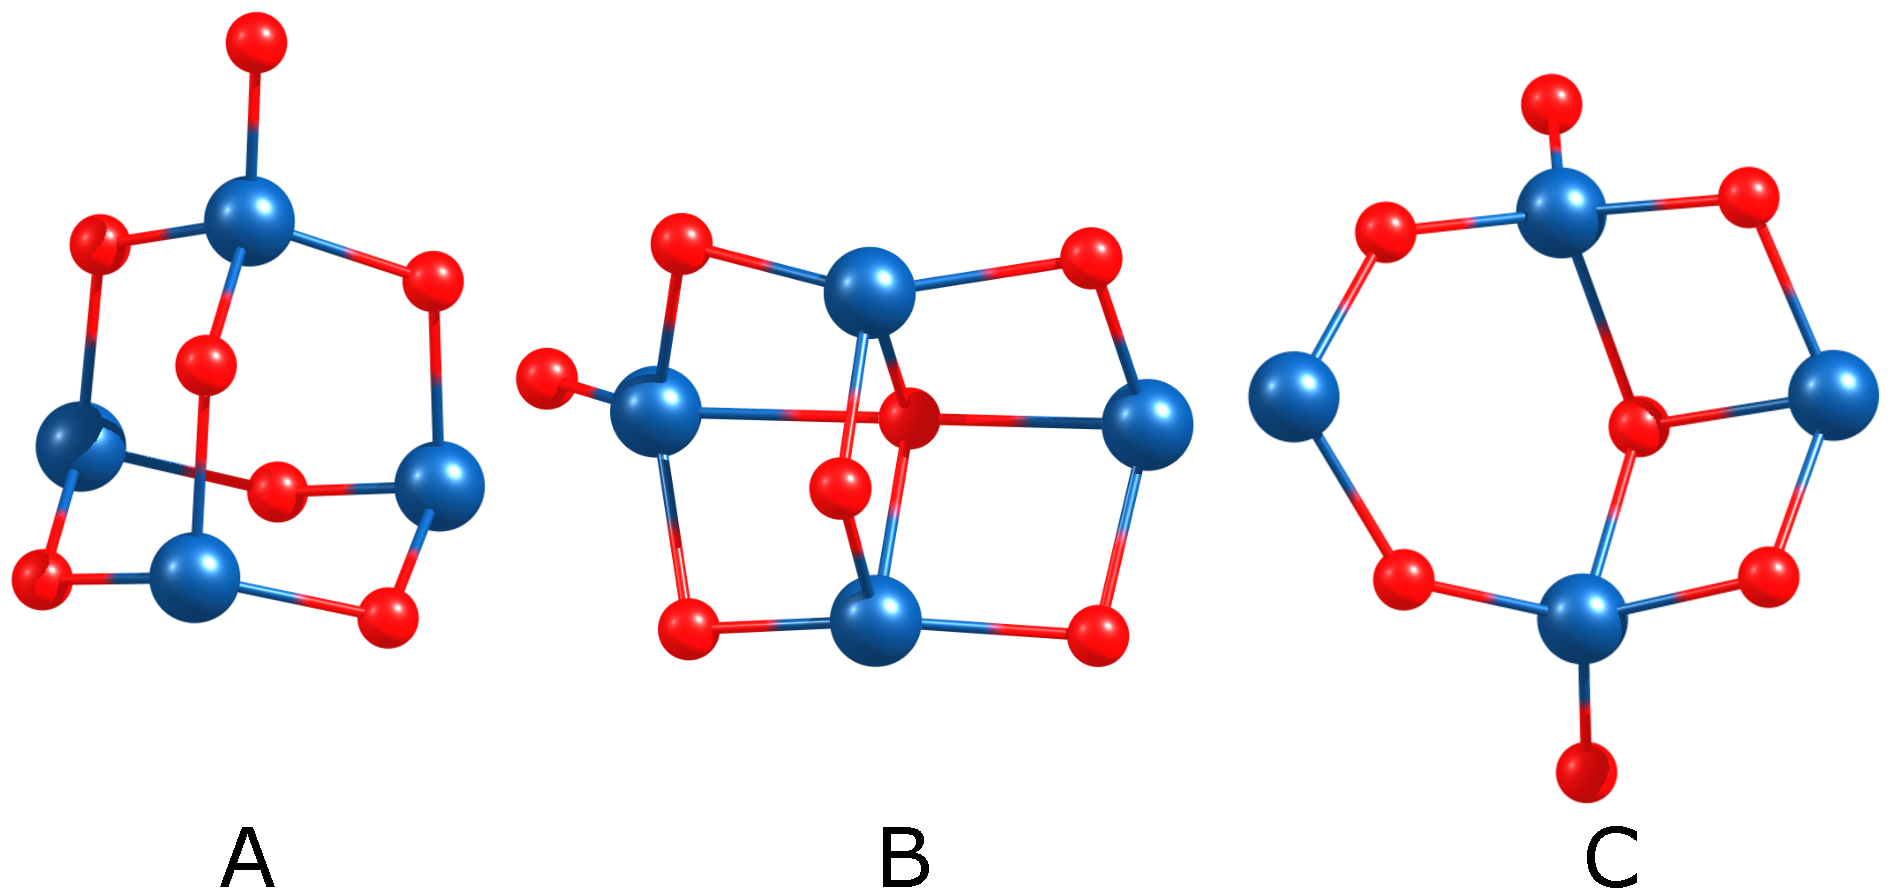
\includegraphics[scale=0.16]{Cr4O7-iso}
	\caption{Geometrical structures of the lowest energy isomers of \ch{Cr4O7+}. The shown structures are obtained with the TPSS/def2TZVP optimizations. Chromium and oxygen atoms are represented as blue and red spheres, respectively.}
	\label{figs:Cr4O7}
\end{figure}




\begin{table}[]
	\centering
	\caption{Relative energies (in eV) of the low energy isomers of \ch{Cr4O8+} calculated at the TPSS level}
	\begin{tabular}{@{}rclc@{}}
	\toprule
	state 	 & isomer & sym. 	& relative energy (eV) \\ \midrule
	$^2$A    & A      & C$_1$   & 0.00                 \\
	$^4$A    & A      & C$_1$   & 0.19                 \\
	$^6$A    & A      & C$_1$   & 0.24                 \\
	$^8$A    & A      & C$_1$   & 0.47                 \\
	$^6$A    & B      & C$_1$   & 1.15                 \\
	$^2$A    & C      & C$_1$   & 1.16                 \\
	$^6$A    & C      & C$_1$   & 1.17                 \\ \bottomrule
	\end{tabular}
\end{table}


\begin{figure}
	\centering
	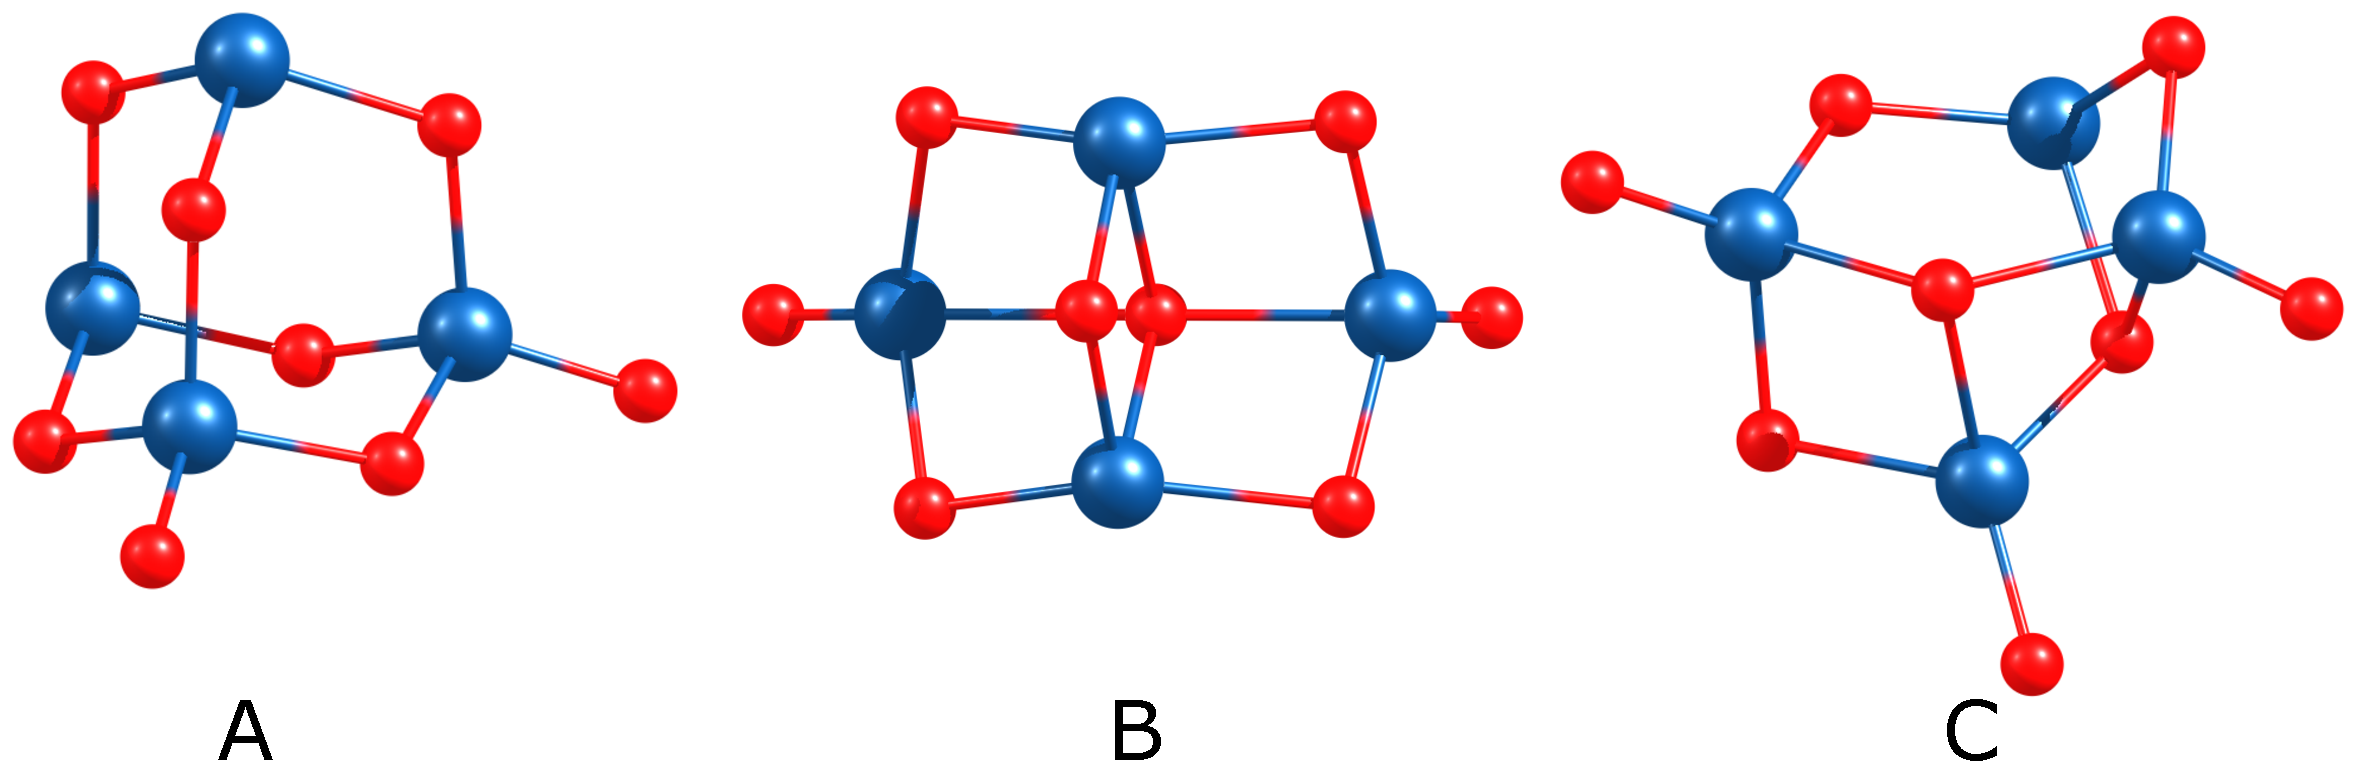
\includegraphics[scale=0.16]{Cr4O8-iso}
	\caption{Geometrical structures of the lowest energy isomers of \ch{Cr4O8+}. The shown structures are obtained with the TPSS/def2TZVP optimizations. Chromium and oxygen atoms are represented as blue and red spheres, respectively.}
	\label{figs:Cr4O8}
\end{figure}




\FloatBarrier



\begin{table}[]
	\centering
	\caption{Relative energies (in eV) of the low energy isomers of \ch{Cr4O9+} calculated at the TPSS level}
	\begin{tabular}{@{}rlc@{}}
	\toprule
	state    & sym.    & relative energy (eV) \\ \midrule
	$^4$A    & C$_1$   & 0.00                 \\
	$^6$A    & C$_1$   & 0.07                 \\
	$^2$A    & C$_1$   & 0.58                 \\ \bottomrule
	\end{tabular}
\end{table}


\begin{table}[]
	\centering
	\caption{Relative energies (in eV) of the low energy isomers of \ch{Cr4O10+} calculated at the TPSS level}
	\begin{tabular}{@{}rlc@{}}
	\toprule
	state    & sym.    & relative energy (eV) \\ \midrule
	$^2$A    & C$_1$   & 0.00                 \\
	$^4$A    & C$_1$   & 0.59                 \\
	$^6$A    & C$_1$   & 3.00                 \\ \bottomrule
	\end{tabular}
\end{table}



\begin{figure}
	\centering
	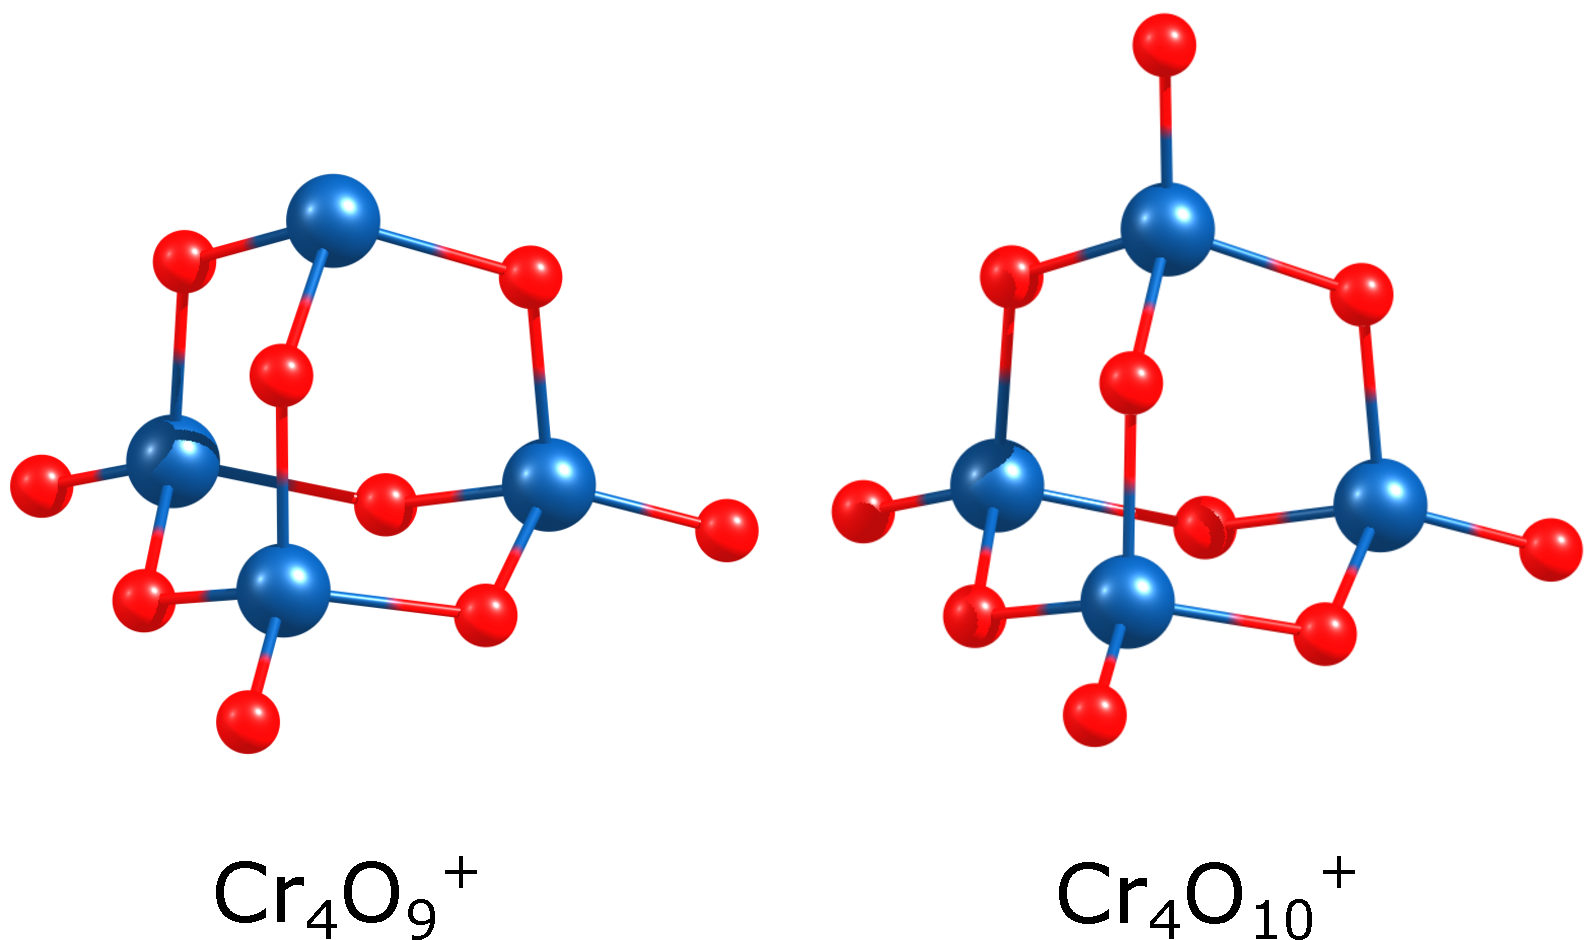
\includegraphics[scale=0.16]{Cr4O9_10-iso}
	\caption{Geometrical structures of the lowest energy isomers of \ch{Cr4O9+} and \ch{Cr4O10+}. The shown structures are obtained with the TPSS/def2TZVP optimizations. Chromium and oxygen atoms are represented as blue and red spheres, respectively.}
	\label{figs:Cr4O9_10}
\end{figure}




\begin{figure}
	\centering
	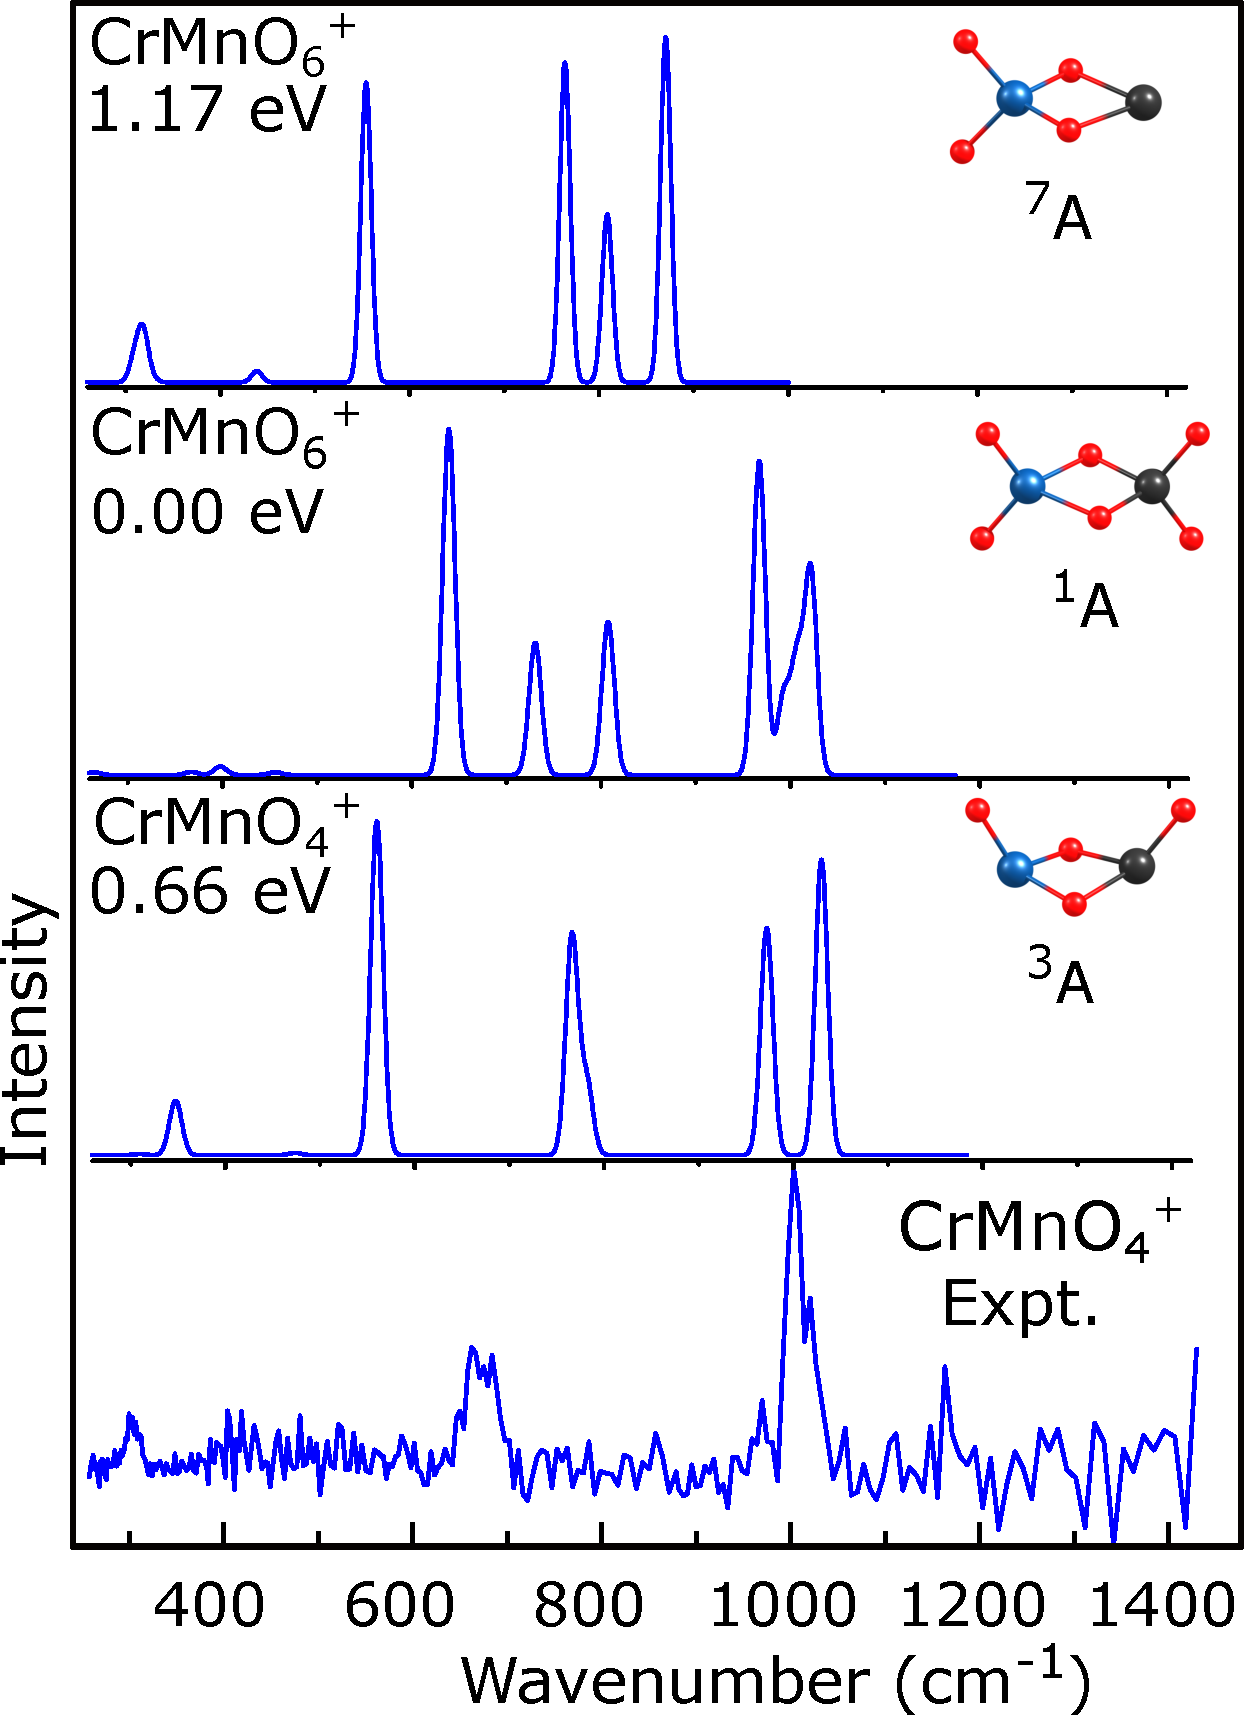
\includegraphics[width=0.4\linewidth]{CrMnO4-spec-si}
	\caption{Experimental IRMPD and simulated harmonic IR spectra of \ch{CrMnO4+} at the TPSS level. The geometrical structures of selected low-lying states are given as inset with chromium (manganese) atoms represented by blue (black) balls. Relative energies are considered within the same molecular sizes.}
	\label{figs:CrMnO4-spec-si}
\end{figure}




\begin{figure}
	\centering
	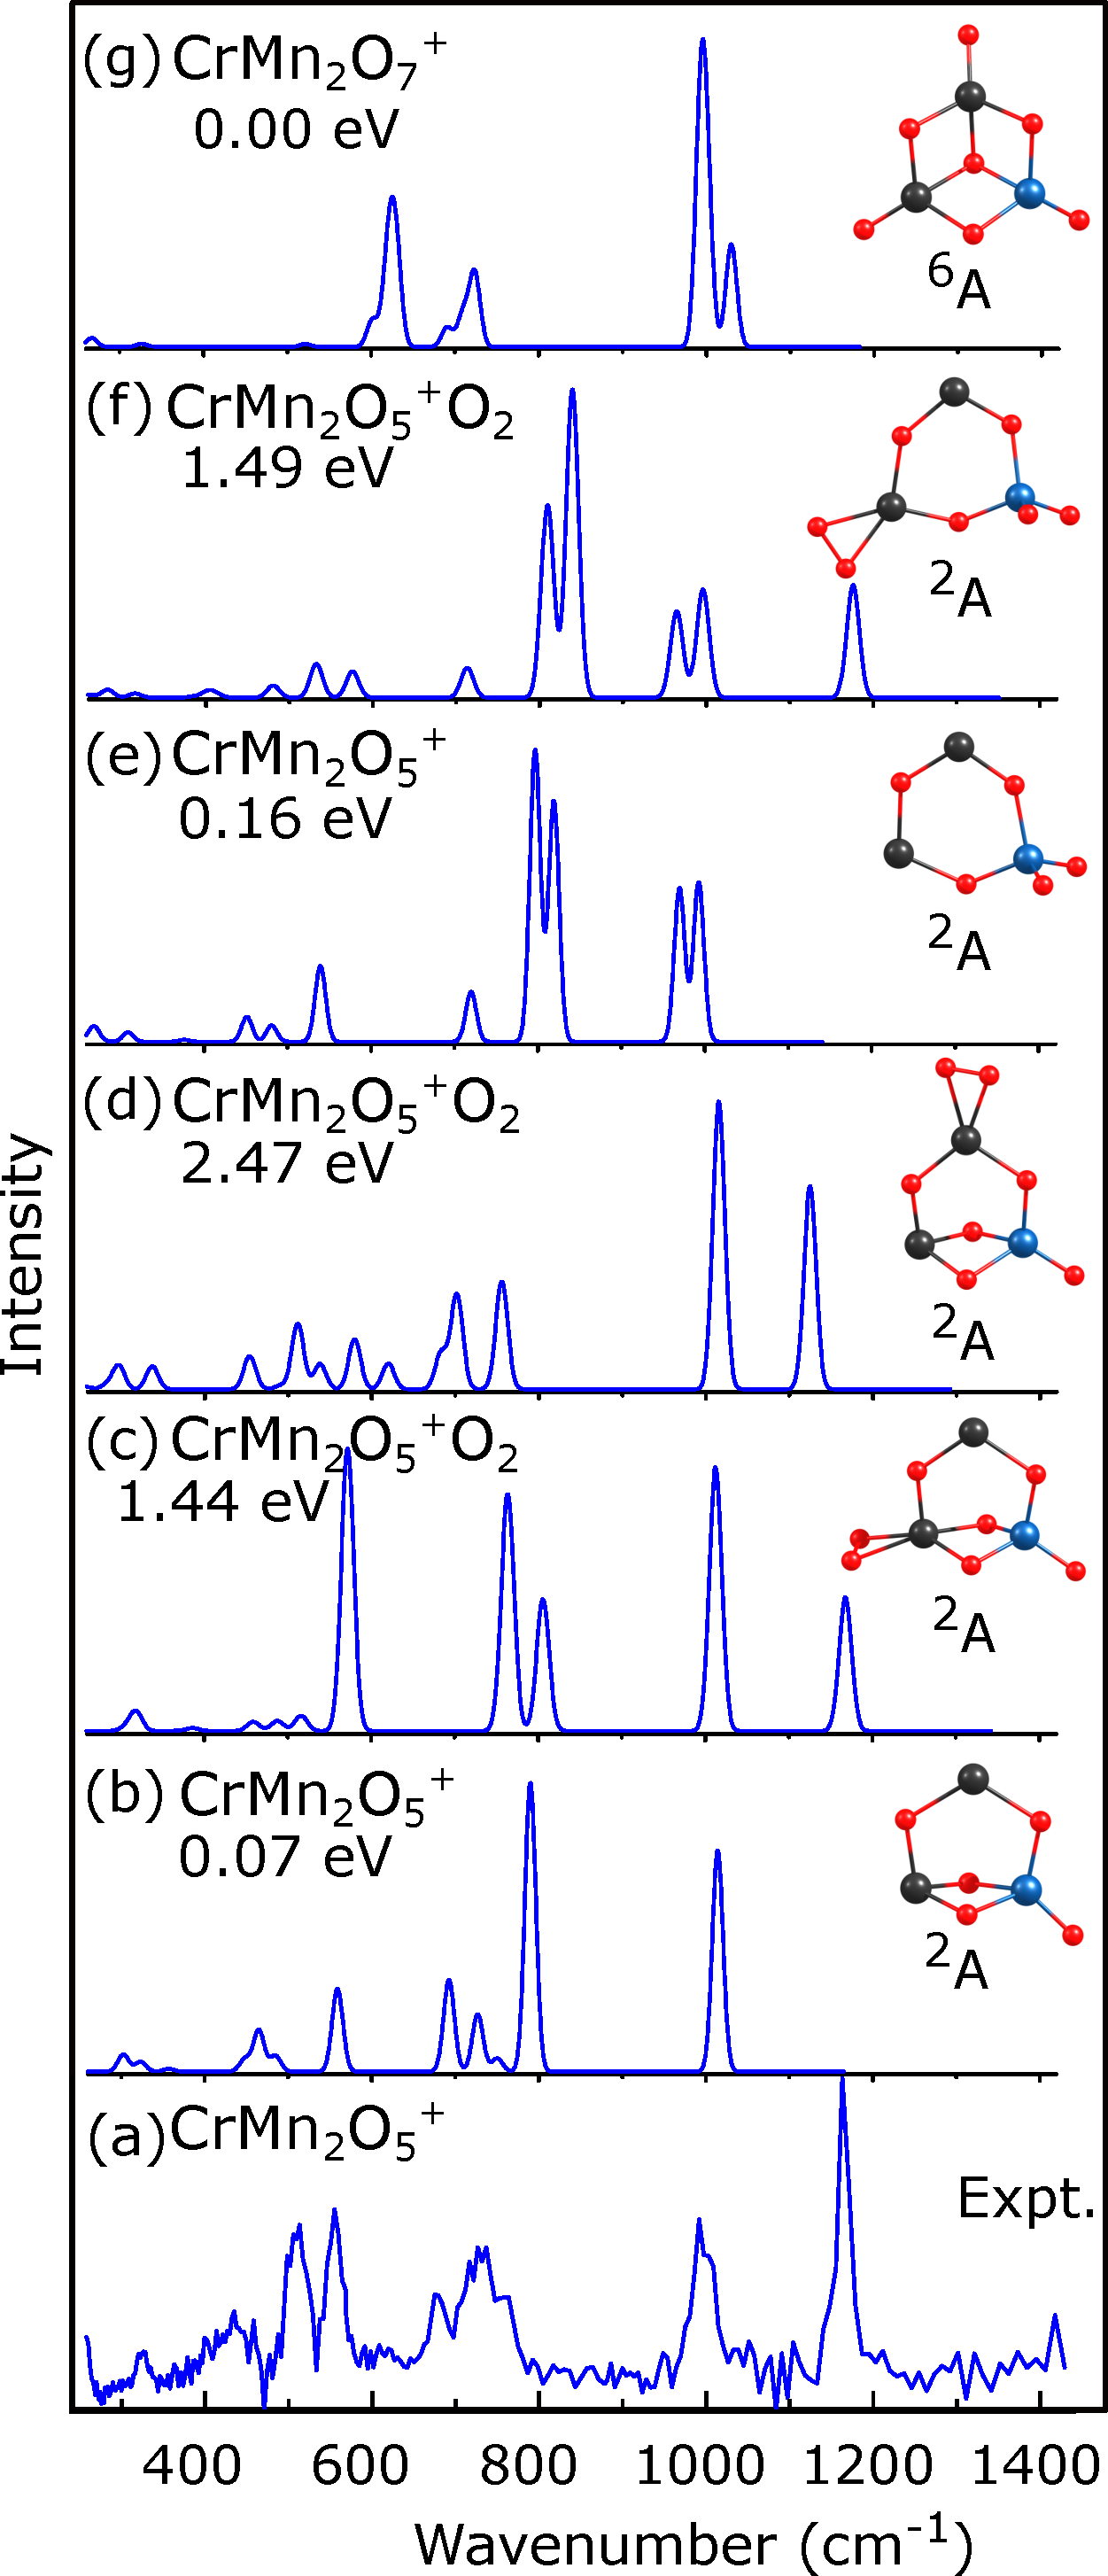
\includegraphics[width=0.4\linewidth]{CrMn2O5-spec-si}
	\caption{Experimental IRMPD and simulated harmonic IR spectra of \ch{CrMn2O5+} and \ch{CrMn2O5^+O2} at the TPSS level. The geometrical structures of selected low-lying states are given as inset with chromium (manganese) atoms represented by blue (black) balls. Relative energies are considered within the same molecular sizes.}
	\label{figs:CrMn2O5-spec-si}
\end{figure}


\begin{figure}
	\centering
	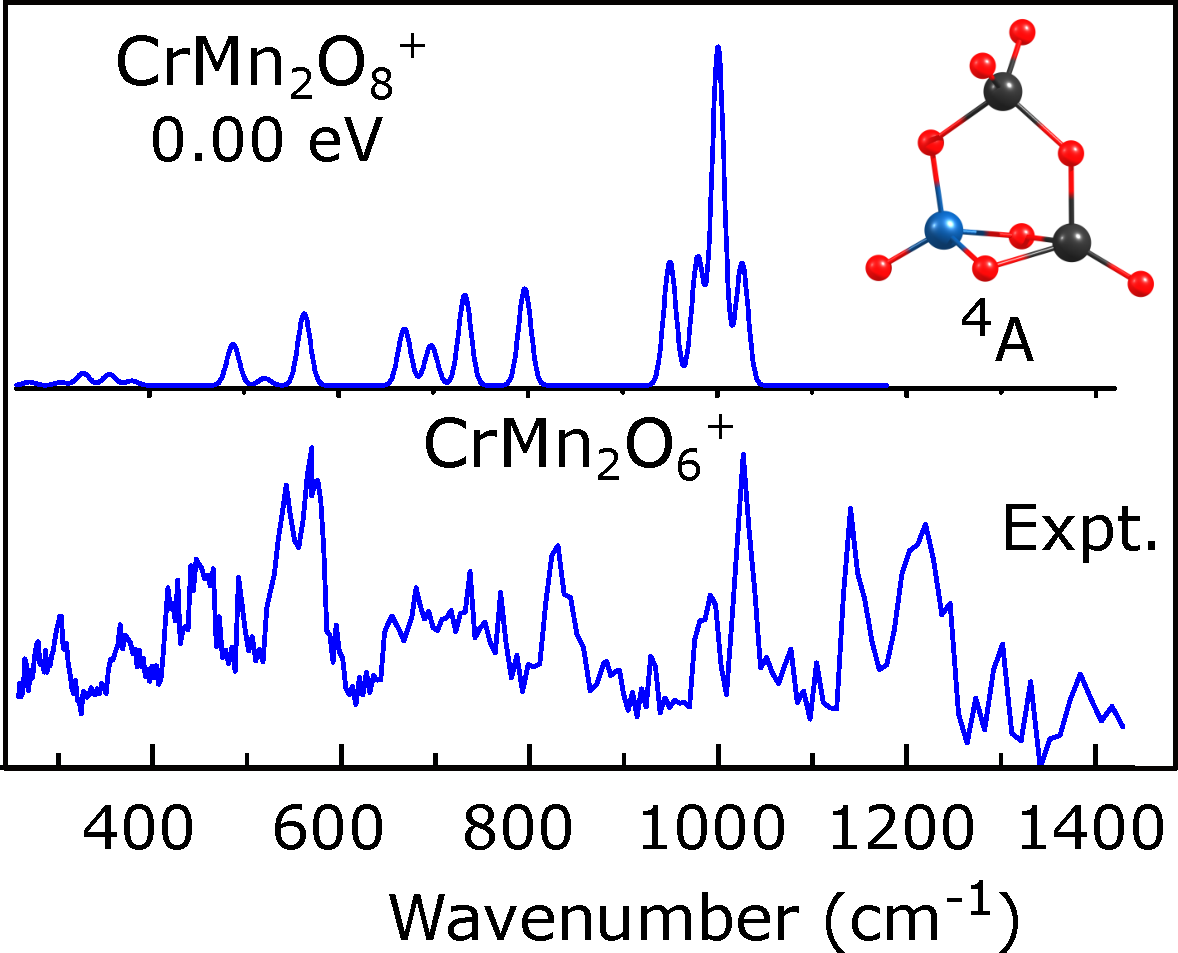
\includegraphics[width=0.4\linewidth]{CrMn2O6-spec-si}
	\caption{Experimental IRMPD and simulated harmonic IR spectra of \ch{CrMn2O8+} at the TPSS level. The geometrical structures of selected low-lying states are given as inset with chromium (manganese) atoms represented by blue (black) balls. Relative energies are considered within the same molecular sizes.}
	\label{figs:CrMn2O5-spec-si}
\end{figure}



\begin{figure}
	\centering
	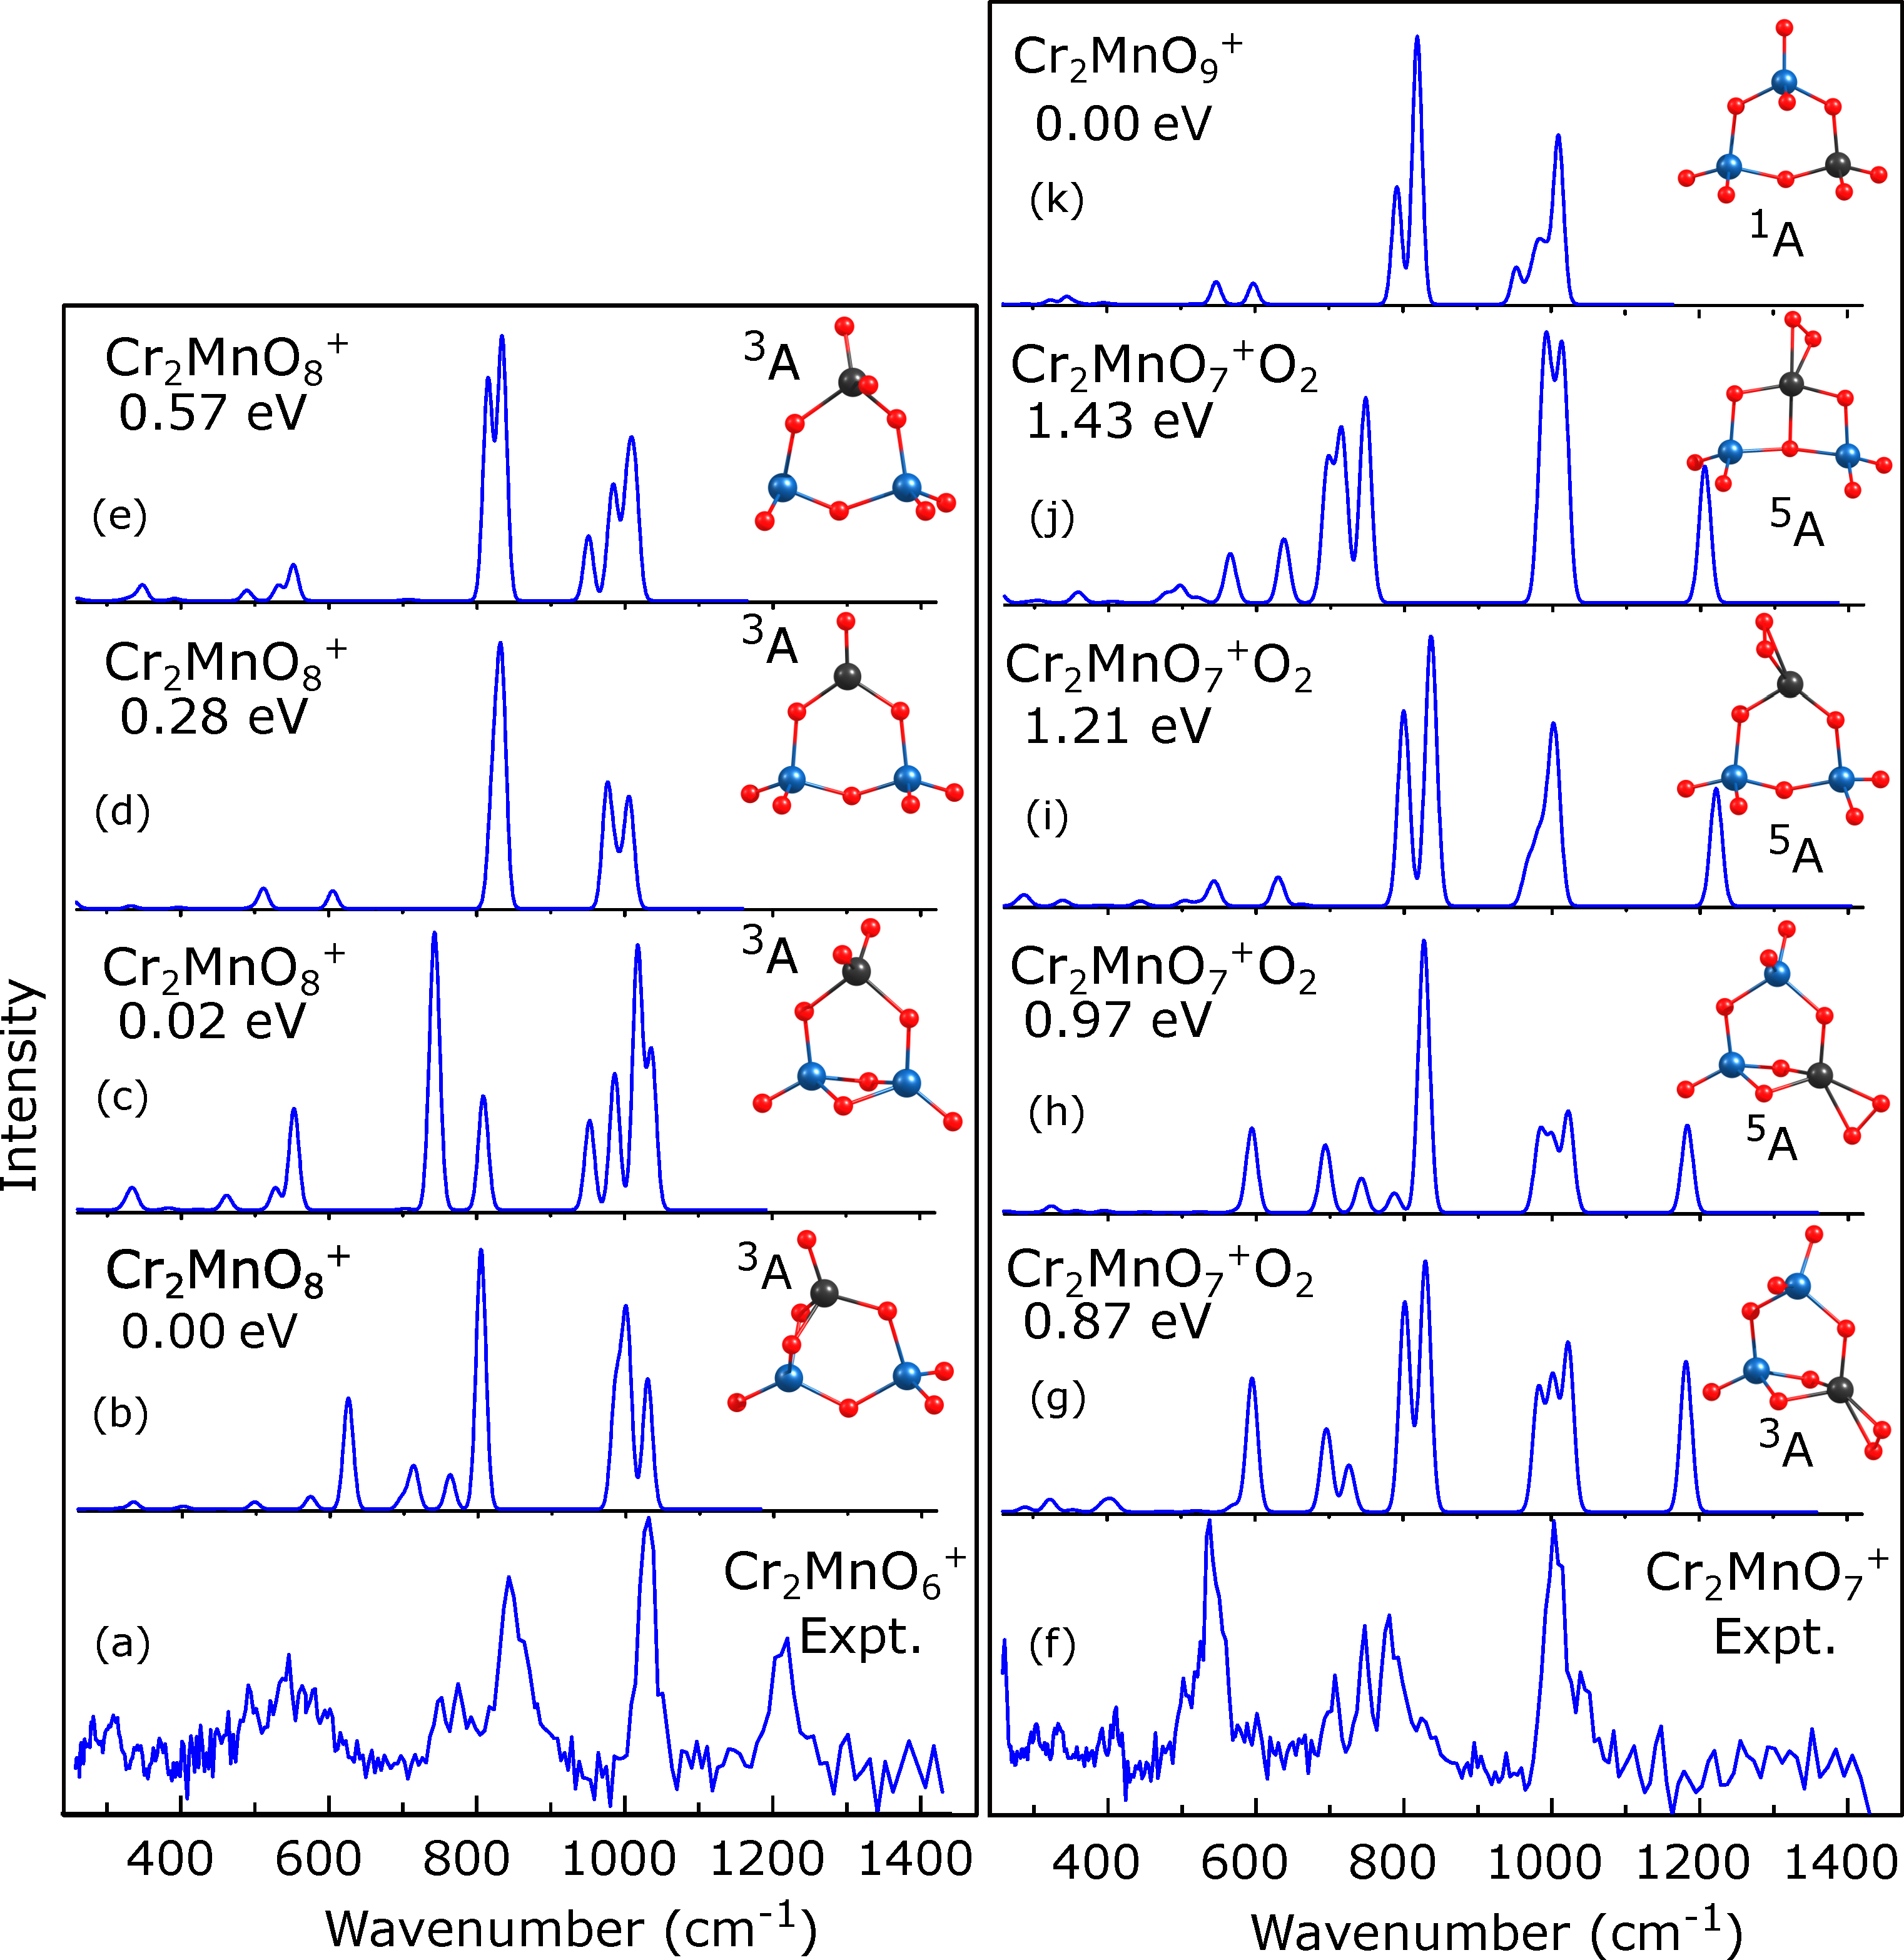
\includegraphics[width=0.95\linewidth]{Cr2MnOz-spec-SI}
	\caption{Experimental IRMPD and simulated harmonic IR spectra of the mother cluster \ch{Cr2MnO8+}, and \ch{Cr2MnO7^+O2} at the TPSS level. The geometrical structures of selected low-lying states are given as inset with chromium (manganese) atoms represented by blue (black) balls. Relative energies are considered within the same molecular sizes.}
	\label{figs:Cr2MnOz-spec-si}
\end{figure}



\begin{figure}
	\centering
	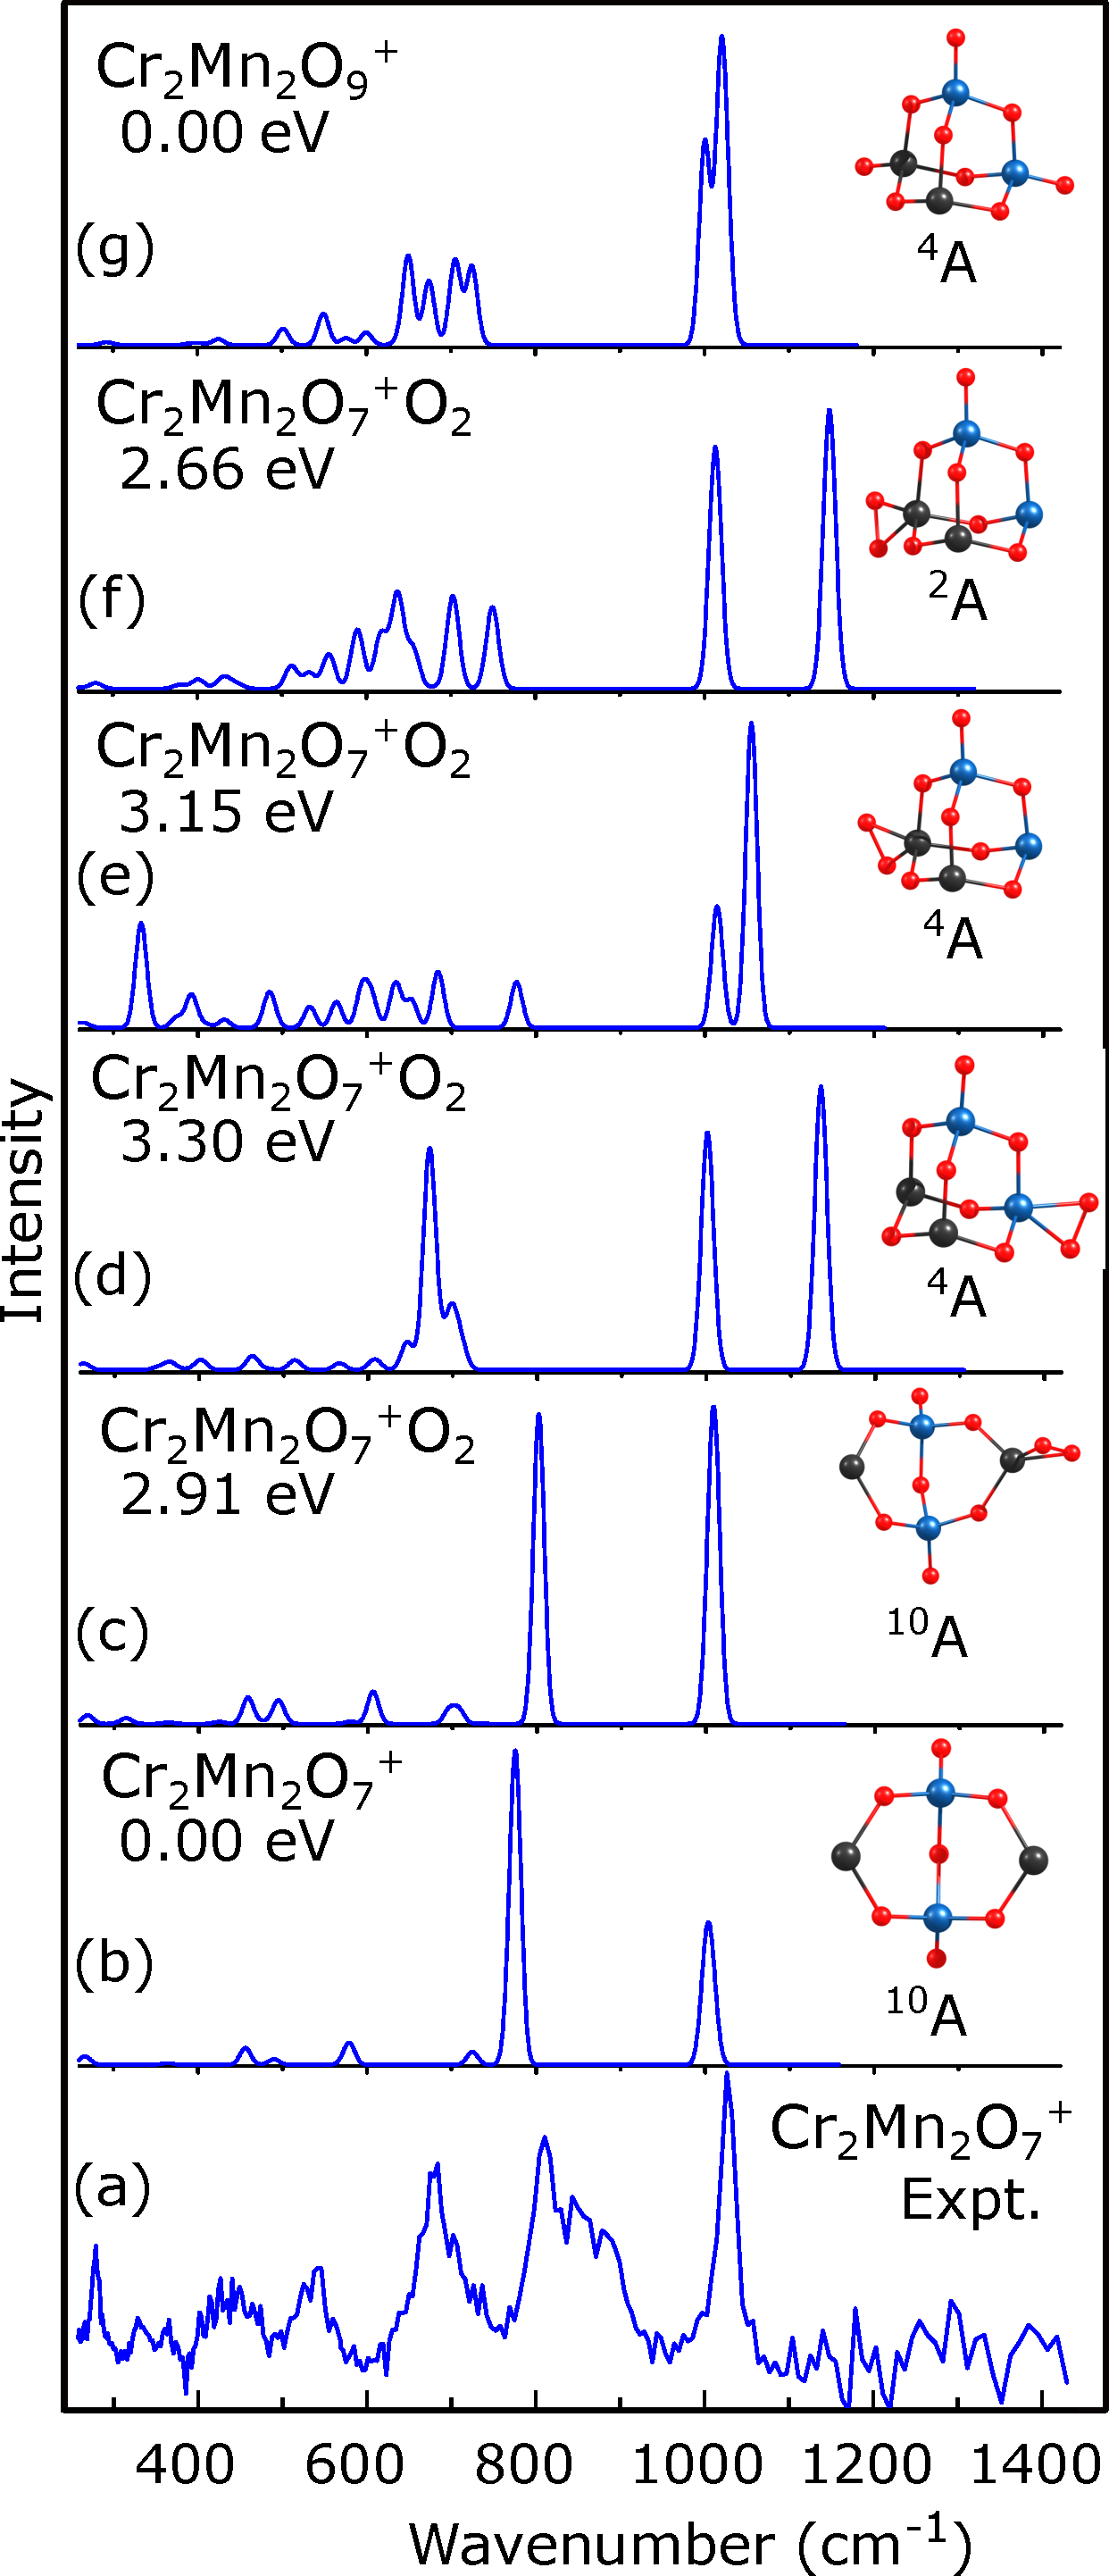
\includegraphics[width=0.4\linewidth]{Cr2Mn2O7-spec-si}
	\caption{Experimental IRMPD and simulated harmonic IR spectra of \ch{Cr2Mn2O7+} and \ch{Cr2Mn2O7^+O2} at the TPSS level. The geometrical structures of selected low-lying states are given as inset with chromium (manganese) atoms represented by blue (black) balls. Relative energies are considered within the same molecular sizes.}
	\label{figs:Cr2Mn2O7-spec-si}
\end{figure}



\begin{figure}
	\centering
	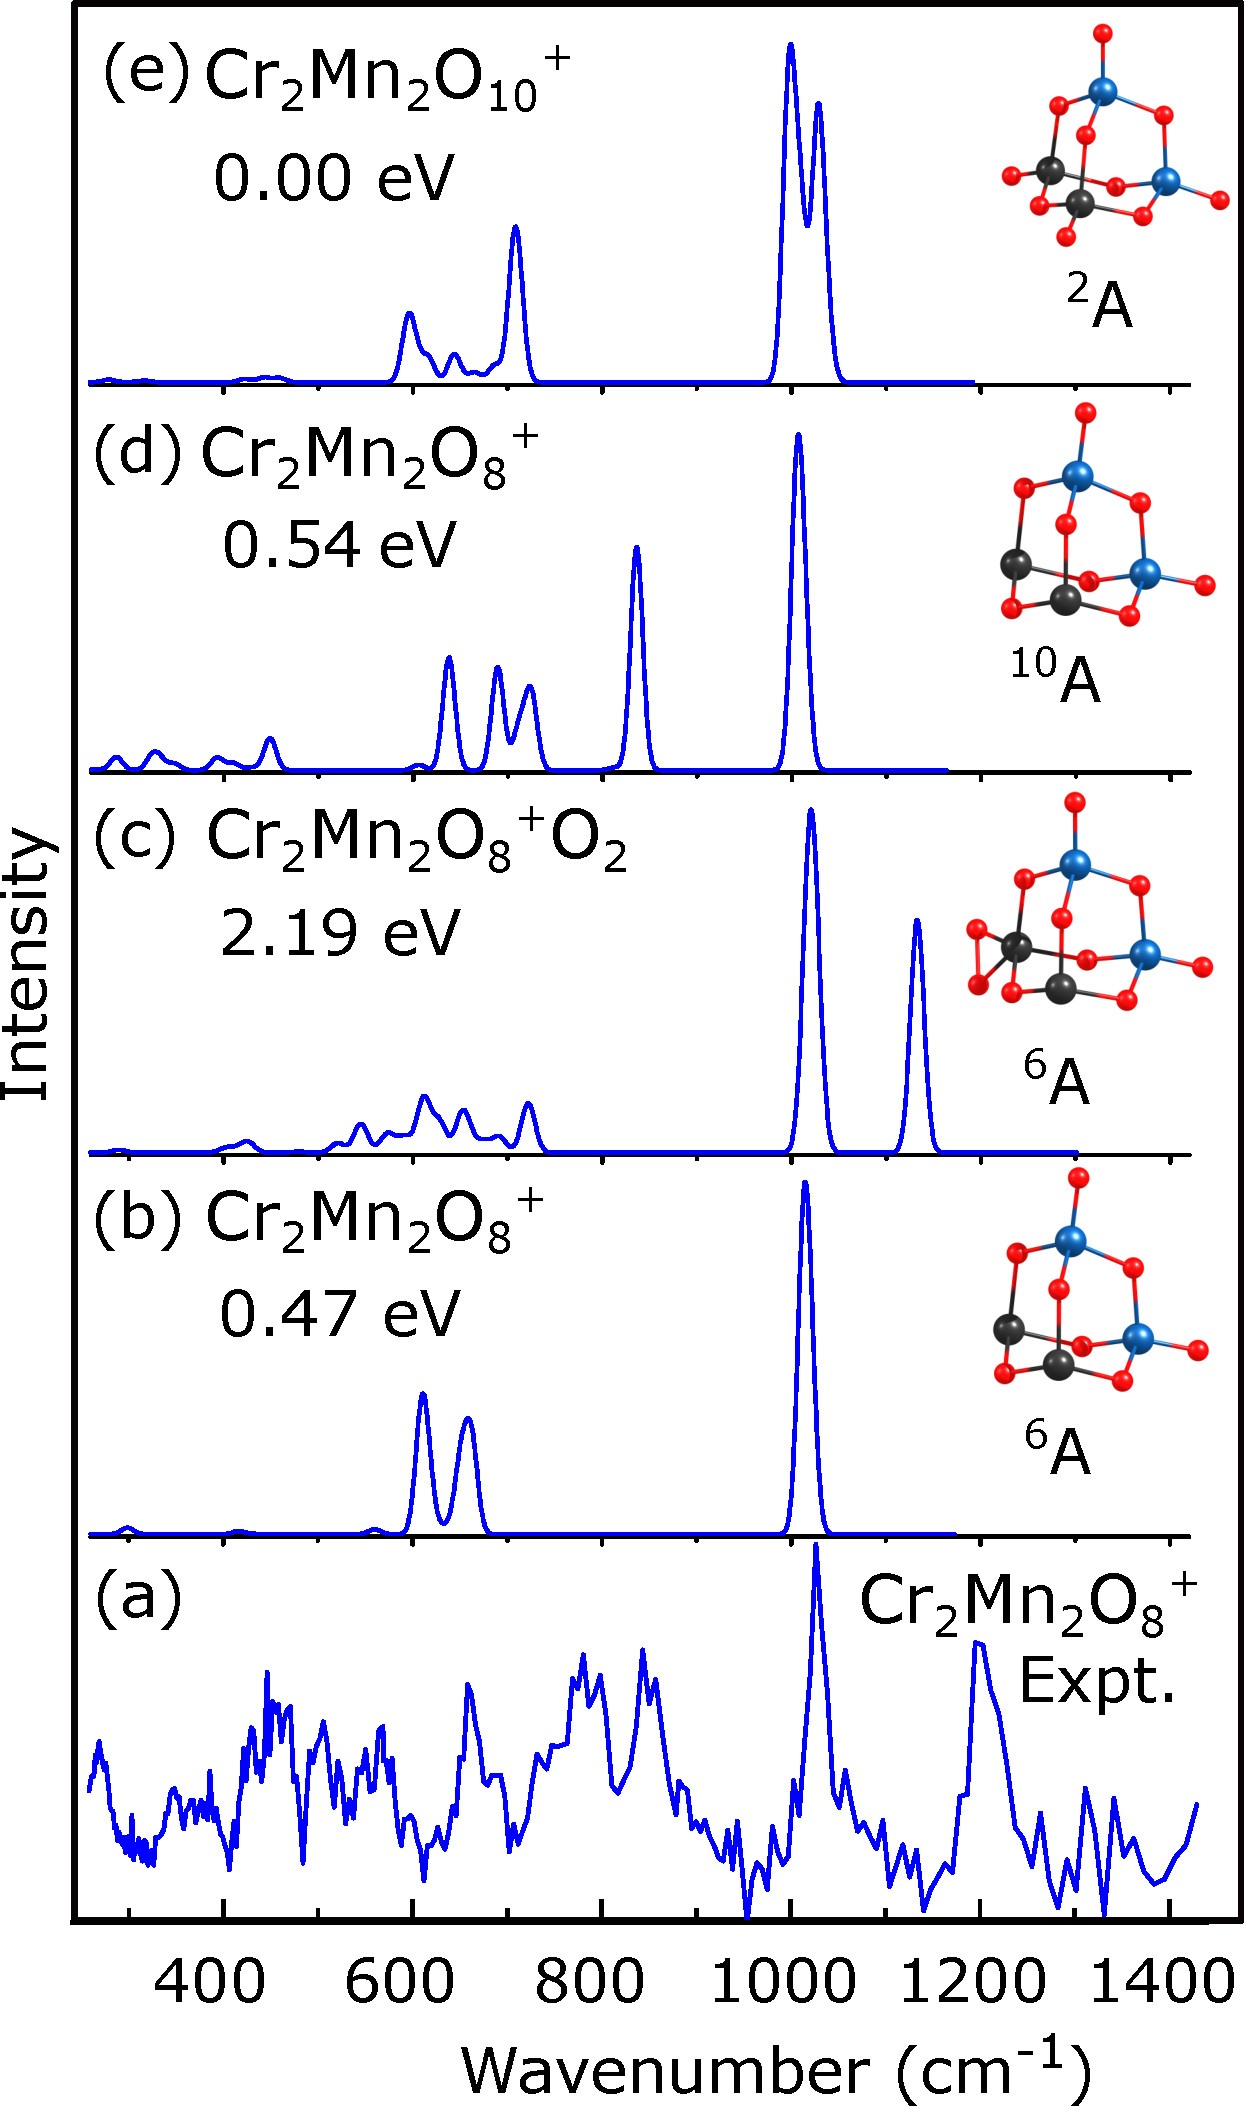
\includegraphics[width=0.4\linewidth]{Cr2Mn2O8-spec-si}
	\caption{Experimental IRMPD and simulated harmonic IR spectra of \ch{Cr2Mn2O8+} and \ch{Cr2Mn2O8^+O2} at the TPSS level. The geometrical structures of selected low-lying states are given as inset with chromium (manganese) atoms represented by blue (black) balls. Relative energies are considered within the same molecular sizes.}
	\label{figs:Cr2Mn2O8-spec-si}
\end{figure}




%\FloatBarrier

\begin{figure}
	\centering
	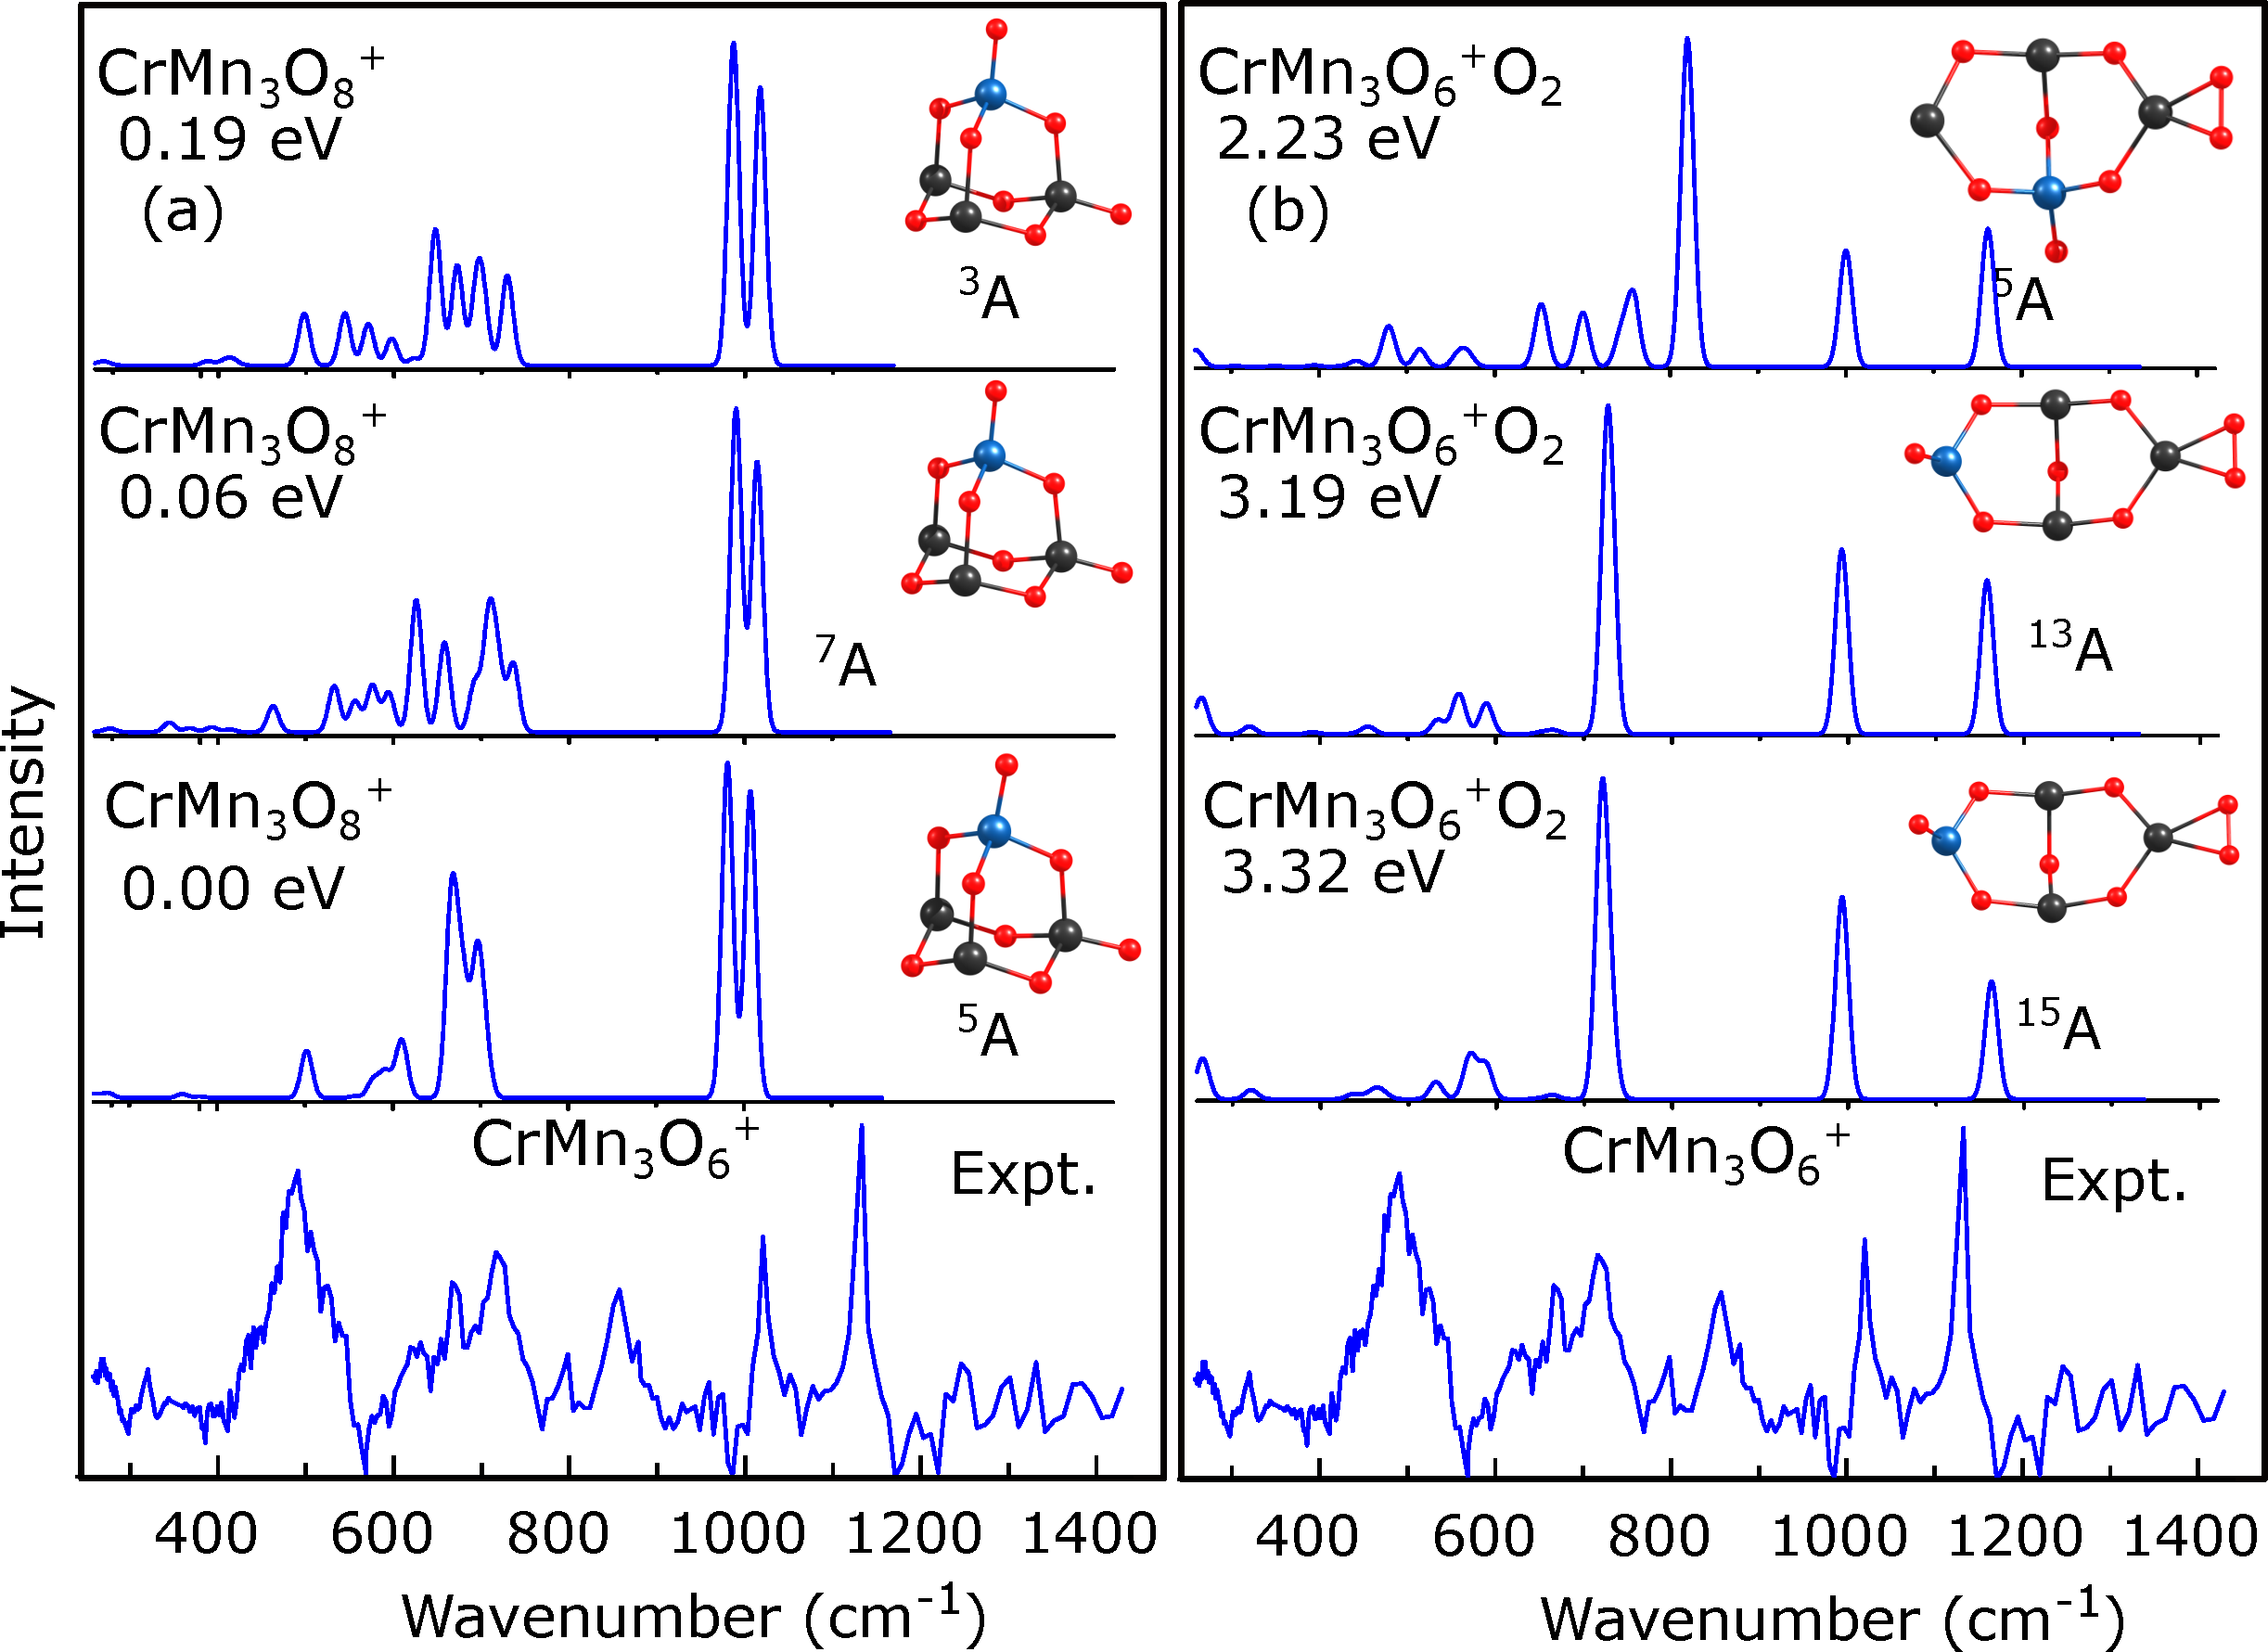
\includegraphics[width=0.95\linewidth]{CrMn3O6-spec-si}
	\caption{Experimental IRMPD and simulated harmonic IR spectra of \ch{CrMn3O6^+O2} and the mother cluster \ch{CrMn3O8+} at the TPSS level. The geometrical structures of selected low-lying states are given as inset with chromium (manganese) atoms represented by blue (black) balls. Relative energies are considered within the same molecular sizes.}
	\label{figs:CrMn3O6-spec-si}
\end{figure}





\begin{figure}
	\centering
	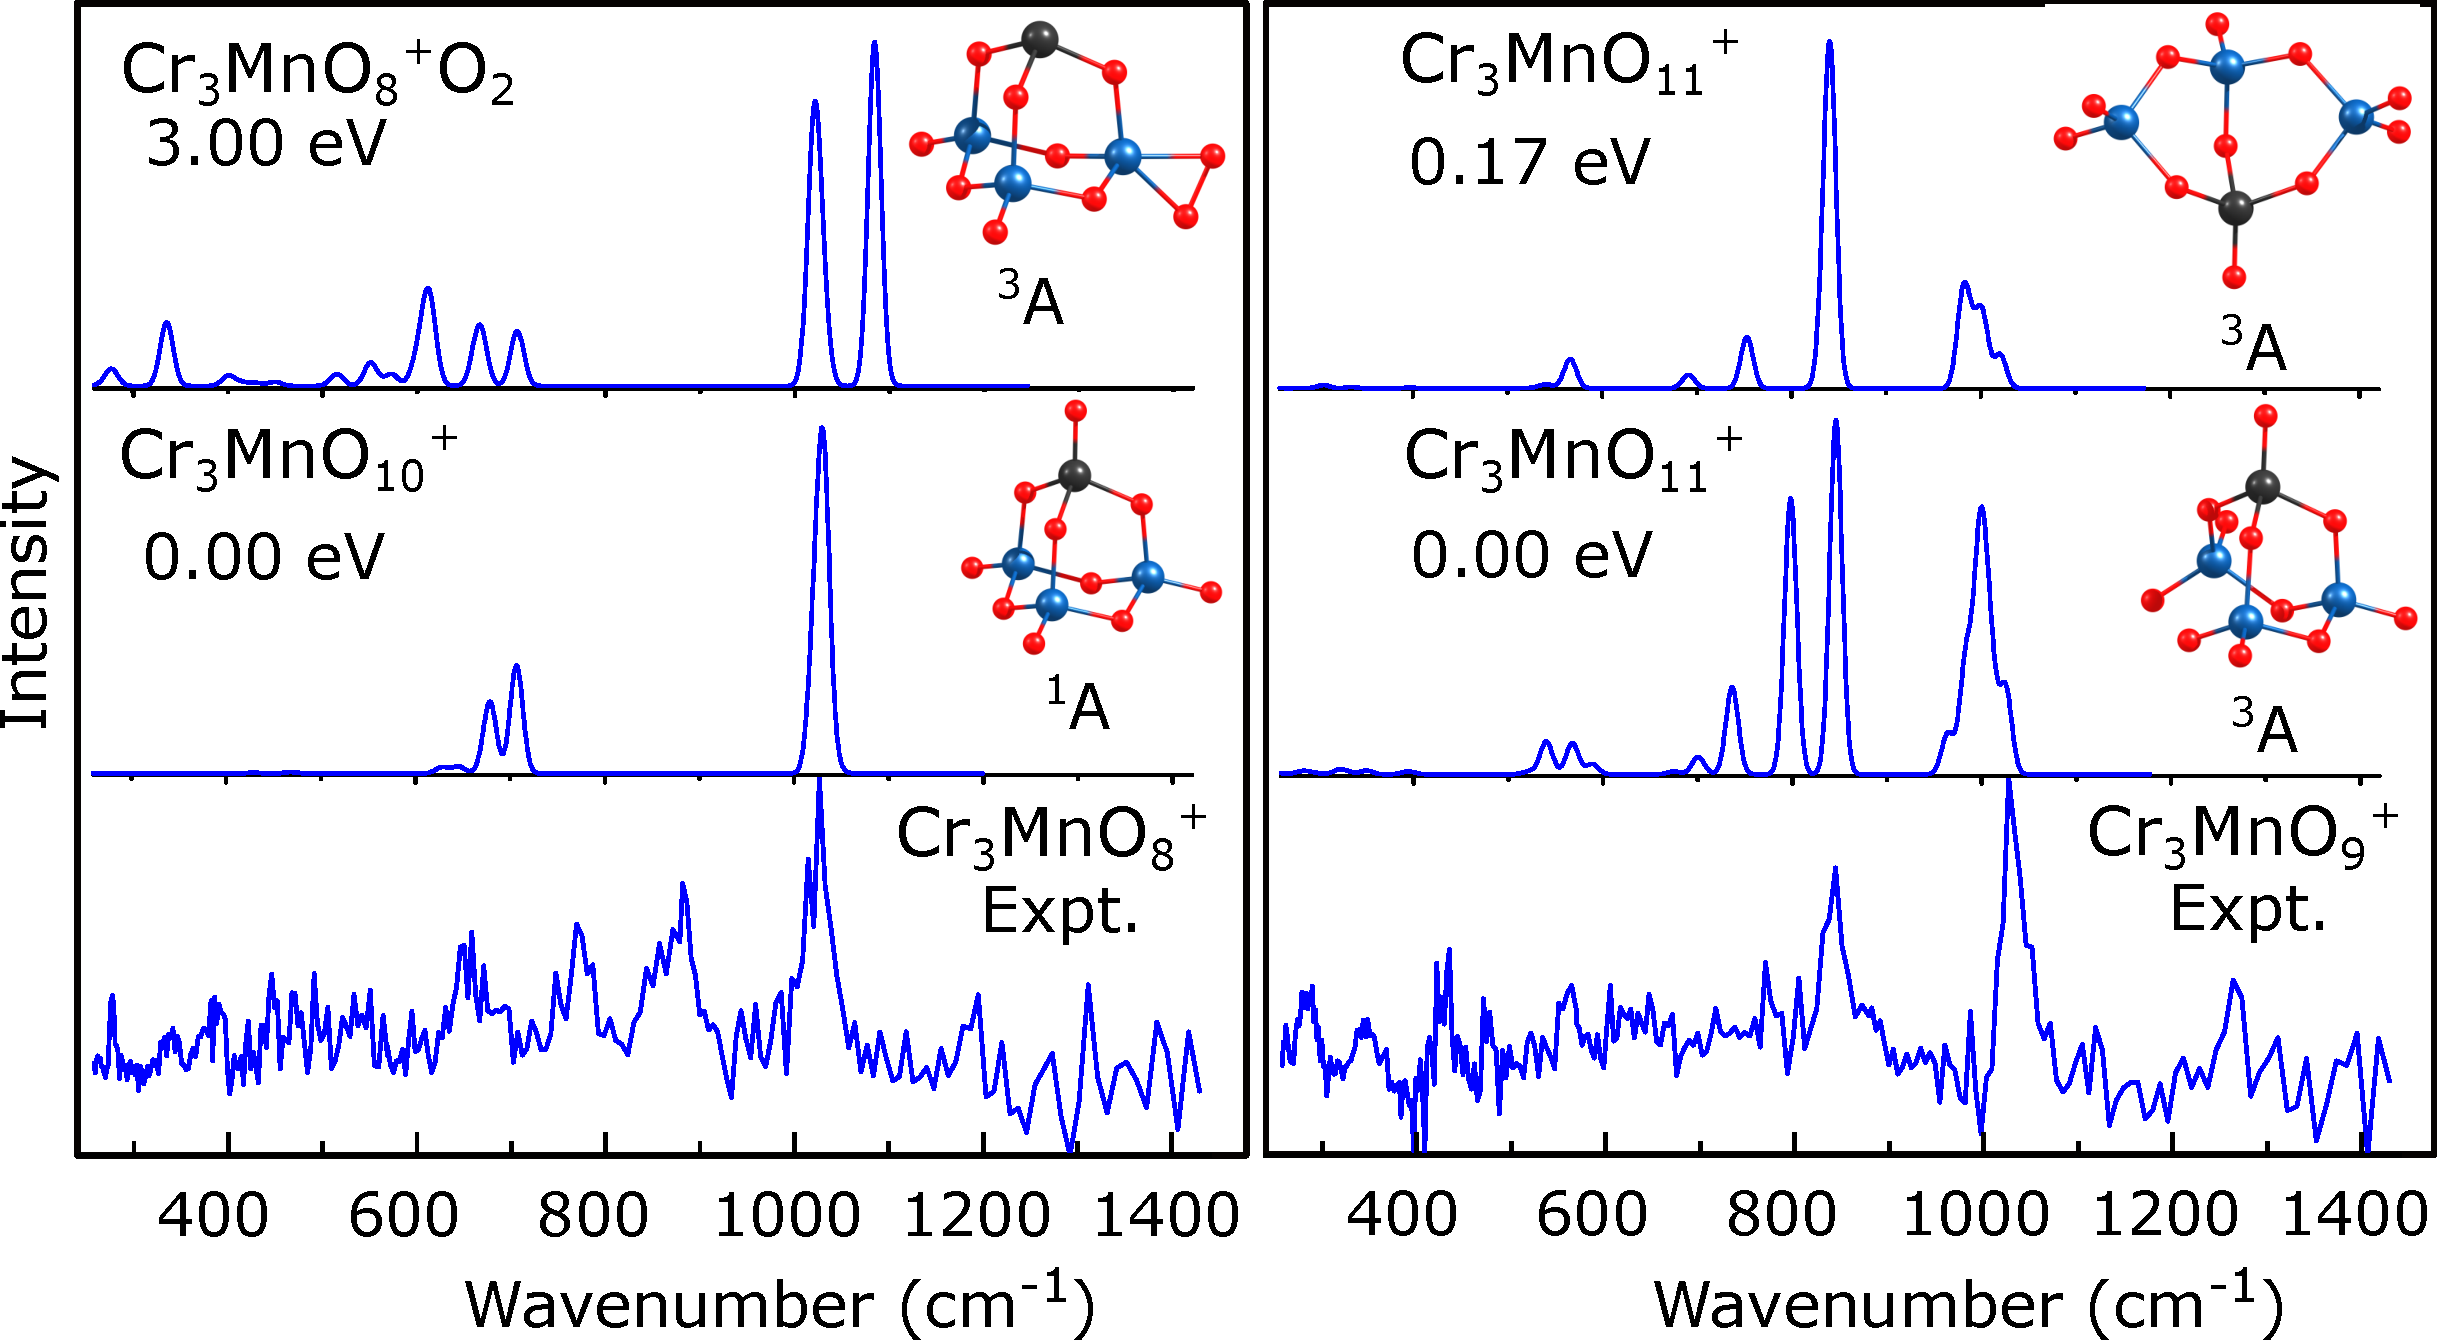
\includegraphics[width=0.95\linewidth]{Cr3MnOz-spec-si}
	\caption{Experimental IRMPD and simulated harmonic IR spectra of \ch{Cr3MnO8^+O2} and the mother cluster \ch{Cr3MnO10}, and the mother cluster \ch{Cr3MnO11} at the TPSS level. The geometrical structures of selected low-lying states are given as inset with chromium (manganese) atoms represented by blue (black) balls. Relative energies are considered within the same molecular sizes.}
	\label{figs:Cr3MnOz-spec-si}
\end{figure}

\FloatBarrier

%\begin{table}[]
%	\centering
%	\caption{Binding energy of the \ch{O2} group on daughter clusters}
%	\begin{tabular}{@{}llcc@{}}
%	\toprule
%	daughter cluster  &  cluster with \ch{O2} group & spin state & binding energy of \ch{O2} (eV) \\ \midrule
%	\ch{CrMnO4+}      &  \ch{CrMnO4^+O2}            & 5          & 1.71                      \\
%	\ch{CrMn2O5+}     &  \ch{CrMn2O5^+O2}           & 4          & 1.87                      \\
%	\ch{CrMn2O6+}     &  \ch{CrMn2O6^+O2}           & 4          & 2.80                      \\
%	\ch{Cr2MnO6+}     &  \ch{Cr2MnO6^+O2}           & 7          & 2.83                      \\
%	\ch{Cr2MnO7+}     &  \ch{Cr2MnO7^+O2}           & 3          & 1.74                      \\
%	\ch{CrMn3O6+}     &  \ch{CrMn3O6^+O2}           & 3          & 1.64                      \\
%	\ch{Cr2Mn2O7+}    &  \ch{Cr2Mn2O7^+O2}          & 2          & 3.18                      \\
%	\ch{Cr2Mn2O8+}    &  \ch{Cr2Mn2O8^+O2}          & 2          & 2.21                      \\
%	\ch{Cr3MnO8+}     &  \ch{Cr3MnO8^+O2}           & 3          & 2.62                      \\
%			 	      &  		                    & 3          & 2.86                      \\
%	\ch{Cr3MnO9+}     &  \ch{Cr3MnO9^+O2}           & 5          & 1.47                      \\ \bottomrule
%	\end{tabular}
%\end{table}


% Please add the following required packages to your document preamble:
% \usepackage{booktabs}
\begin{table}[htb!]
	\centering
	\caption{Local magnetic moments of metallic sites in \ch{Cr4O6+}, \ch{Cr3MnO6+}, \ch{Cr2Mn2O6+}, \ch{CrMn3O6+}}
	\label{tab:localmaget}
	\begin{tabular}{@{}lllll@{}}
	\toprule
		cluster    & \multicolumn{4}{c}{metallic site}            \\ \midrule
	\ch{Cr4O6+}    & Cr1: 2.1  & Cr2: 2.9  & Cr3: 2.1  & Cr4: 2.1 \\
	\ch{Cr3MnO6+}  & Cr1: 2.0  & Cr2: 2.79 & Cr3: 2.0 & Mn4: 3.3 \\
	\ch{Cr2Mn2O6+} & Cr1: -1.6 & Cr2: -1.4 & Mn3: 2.1  & Mn4: 3.9 \\
	\ch{CrMn3O6+}  & Cr1: -0.6 & Mn2: 0.61 & Mn3: -2.1 & Mn4: 4.1 \\ \bottomrule
	\end{tabular}
	\end{table}




	